%%
%% This is file `sample-acmlarge.tex',
%% generated with the docstrip utility.
%%
%% The original source files were:
%%
%% samples.dtx  (with options: `acmlarge')
%% 
%% IMPORTANT NOTICE:
%% 
%% For the copyright see the source file.
%% 
%% Any modified versions of this file must be renamed
%% with new filenames distinct from sample-acmlarge.tex.
%% 
%% For distribution of the original source see the terms
%% for copying and modification in the file samples.dtx.
%% 
%% This generated file may be distributed as long as the
%% original source files, as listed above, are part of the
%% same distribution. (The sources need not necessarily be
%% in the same archive or directory.)
%%
%% The first command in your LaTeX source must be the \documentclass command.
\documentclass[acmsmall]{acmart}
% \documentclass[acmlarge]{acmart}
% \documentclass[manuscript,review]{acmart}
% \documentclass[sigchi]{acmart}



\usepackage{colortbl}
\usepackage{multirow}
\usepackage{enumitem}
\usepackage{booktabs}
\usepackage{makecell}
\usepackage{lscape}
\usepackage{caption}
\usepackage{subcaption}
\usepackage{icomma}


\usepackage{acronym}
\newacro{WHO-5}{World Health Organization-Five Well-Being Index}
\newacro{BFI-10} {Big Five Inventory‐10}
\newacro{UEQ} {User Experience Questionnaire}
\newacro{PTSD}{Post-traumatic Stress Disorder}
\newacro{PMDD}{Premenstrual Dysphoric Disorder}
\newacro{OCD}{Obsessive Compulsive Disorder}
\newacro{AD}{Affective Disorder}
\newacro{PHQ-9}{Patient Health Questionnaire}
\newacro{GUI}{graphical user interface}
\newacro{CUI}{Conversational User Interface}
\newacro{VUI}{Voice User Interface}
\newacro{VA}{Virtual Assistant}
\newacro{CA}{Conversational Agent}
\newacro{CBT}{Cognitive Behavioral Therapy}
\newacro{BA}{Behavioral Activation}
\newacro{CHA}{Conversational Health Agent}
\newacro{IVR}{Interactive Voice Response}
\newacro{IPA}{Interactive Personal Assistant}
\newacro{VAS}{Virtual Assistant Surface}
\newacro{HIPPA}{Health Insurance Portability and Accountability Act}
\newacro{NLP} {Natural Language Processing}
\newacro{HCI}{Human-Computer Interaction}
\newacro{CHI} {Computer Human Interaction}
\newacro{CSCW} {Computer-supported Cooperative Work}
\newacro{EMA}{Ecological Momentary Assessment}
\newacro{SASSI} {Subjective Assessment of Speech-system Interface Usability}
\newacro{ASR} {Automatic Speech Recognition}
\newacro{RMSE} {Root-mean-square error}
\newacro{ASK} {Alexa Skills Kit}
\newacro{SDK} {Software Development Kit}
\newacro{AI} {Artificial Intelligence}
\newacro{UX} {User Experience}
\newacro{STM} {Structural Topic Model}
\newacro{LDA}{Latent Dirichlet Allocation}
\newacro{CTM}{Correlated Topic Model}
\newacro{ASIN}{Amazon Standard Identification Number}
\newacro{SSML} {Speech Synthesis Markup Language}
\newacro{GDPR} {General Data Protection Regulation}
\newacro{CACHET} {Copenhagen Center For Health Technology}

\newacro{app} {\textit{Sofia}}



% create a shortcuts
\newcommand\annonymize[1]{Annonymized}

%%
%% \BibTeX command to typeset BibTeX logo in the docs
\AtBeginDocument{%
  \providecommand\BibTeX{{%
    \normalfont B\kern-0.5em{\scshape i\kern-0.25em b}\kern-0.8em\TeX}}}

%% Rights management information.  This information is sent to you
%% when you complete the rights form.  These commands have SAMPLE
%% values in them; it is your responsibility as an author to replace
%% the commands and values with those provided to you when you
%% complete the rights form.
\setcopyright{acmcopyright}
\copyrightyear{2020}
\acmYear{2020}
\acmDOI{10.1145/1122445.1122456}


%%
%% These commands are for a JOURNAL article.
\acmJournal{POMACS}
\acmVolume{1}
\acmNumber{1}
\acmArticle{111}
\acmMonth{1}

%%
%% Submission ID.
%% Use this when submitting an article to a sponsored event. You'll
%% receive a unique submission ID from the organizers
%% of the event, and this ID should be used as the parameter to this command.
%%\acmSubmissionID{123-A56-BU3}

%%
%% The majority of ACM publications use numbered citations and
%% references.  The command \citestyle{authoryear} switches to the
%% "author year" style.
%%
%% If you are preparing content for an event
%% sponsored by ACM SIGGRAPH, you must use the "author year" style of
%% citations and references.
%% Uncommenting
%% the next command will enable that style.
%%\citestyle{acmauthoryear}

%%
%% end of the preamble, start of the body of the document source.
\begin{document}

%%
%% The "title" command has an optional parameter,
%% allowing the author to define a "short title" to be used in page headers.

% MAX WORDS 50
% \title[Perspectives on self-reporting of mental health and wellbeing]{Perspectives on self-reporting of mental health and wellbeing through speech-enabled conversational agents: in the wild study}

% \title{Perspectives on conversational agents supporting the self-reports of mental health and wellbeing: in the wild study}

%\title{Design considerations for conversational agents to support self-report of mental health and wellbeing: in the wild study}

% \title[Conversational Agents for Mental Health Self-reports]{Conversational Agents for Mental Health Self-reports: In the Wild Study  with People Living with Mental Illness}

% \title[Conversational Agents for Mental Health Self-reports]{Conversational Agents for Mental Health Self-reports as Experienced by People Living with Mental Illness}

% \title[Conversational Agents for Mental Health Self-reports]{Conversational Agents for Mental Health Self-reports as Experienced by People Living with Affective Disorders}

%Kevin% \title[The Self-Report of Mental Health via Conversational Agent As Experienced by People Living with Mental Illness]{The Self-Report of Mental Health via Conversational Agent As Experienced by People Living with Mental Illness: An In The Wild Study}

%Jakob% \title[Self-Reporting of Mental Health via a Conversational Agent]{Self-Reporting of Mental Health via a Conversational Agent: A Qualitative Study of the SOFIA System}

\title[A CA for the Self-Report of Wellbeing Among People Living with AD]{Experiences of a Conversational Agent for the Self-Report of Wellbeing Among People Living with Affective Disorders: An In-The-Wild Study}


% \title[]{Speech-Enabled Conversational Agent for the Self-Report of Mental Health and Wellbeing as Experienced by People Living with Affective Disorders: An In-The-Wild Study}

%
% The "author" command and its associated commands are used to define
% the authors and their affiliations.
% Of note is the shared affiliation of the first two authors, and the
% "authornote" and "authornotemark" commands
% used to denote shared contribution to the research.
% \author{Raju Maharjan, Darius Adam Rohani, Kevin Doherty, Per B{\ae}kgaard, Jakob E. Bardram}

% \email{{rajm, daroh, kevdoh, pgba, jakba}@dtu.dk}
% \affiliation{%
%   \institution{Technical University of Denmark}
%   \streetaddress{Anker Engelunds Vej 1}
%   \city{Kgs. Lyngby}
% %   \state{Copenhagen}
%   \postcode{2800}
%   \country{Denmark}
% }

\author{Raju Maharjan}
%\authornote{Both authors contributed equally to this research.}
\email{rajm@dtu.dk}
\orcid{0000-0003-1390-8758}
\affiliation{%
  \institution{Department of Health Technology, Technical University of Denmark}
  \streetaddress{{\O}rsted Plads}
  \city{Kgs. Lyngby}
  \postcode{DK-2800}
  \country{Denmark}
}
\author{Darius Adam Rohani}
%\authornote{Both authors contributed equally to this research.}
\email{daroh@dtu.dk}
\orcid{0000-0003-1390-8758}
\affiliation{%
  \institution{Department of Health Technology, Technical University of Denmark}
  \streetaddress{{\O}rsted Plads}
  \city{Kgs. Lyngby}
  \postcode{DK-2800}
  \country{Denmark}
}
\author{Kevin Doherty}
%\authornote{Both authors contributed equally to this research.}
\email{kevdoh@dtu.dk}
\orcid{0000-0003-1390-8758}
\affiliation{%
  \institution{Department of Health Technology, Technical University of Denmark}
  \streetaddress{{\O}rsted Plads}
  \city{Kgs. Lyngby}
  \postcode{DK-2800}
  \country{Denmark}
}
\author{Per B{\ae}kgaard}
%\authornote{Both authors contributed equally to this research.}
\email{pgba@dtu.dk}
\orcid{0000-0003-1390-8758}
\affiliation{%
  \institution{Department of Applied Mathematics and Computer Science, Technical University of Denmark}
  \streetaddress{Richard Pedersens Plads}
  \city{Kgs. Lyngby}
  \postcode{DK-2800}
  \country{Denmark}
}

\author{Jakob E.~Bardram}
%\authornote{Both authors contributed equally to this research.}
\email{jakba@dtu.dk}
\orcid{0000-0003-1390-8758}
\affiliation{%
  \institution{Department of Health Technology, Technical University of Denmark}
  \streetaddress{{\O}rsted Plads}
  \city{Kgs. Lyngby}
  \postcode{DK-2800}
  \country{Denmark}
}


%%
%% By default, the full list of authors will be used in the page
%% headers. Often, this list is too long, and will overlap
%% other information printed in the page headers. This command allows
%% the author to define a more concise list
%% of authors' names for this purpose.

% \renewcommand{\shortauthors}{Maharjan, et al.}

%%
%% The abstract is a short summary of the work to be presented in the
%% article.
\begin{abstract}
    % MAX WORDS 400 
Self-reports obtained by health questionnaires and diary logs are considered effective methods of monitoring and assessing affective disorders (ADs) including depression and bipolar disorder. While long-established, these methods however represent only one, and potentially limited, means of insight into individuals' experiences. 
% 
The growing commercial success of smart speaker devices following recent advancements in speech recognition technology has surfaced new opportunities for collecting self-reported health and wellbeing data. Speech-enabled conversational agents (CAs) in particular, deployed in home environments using just such systems, may offer increasingly intuitive and engaging means of self-report. To date, however, few real-world studies have examined users' experiences of engaging in the self-report of mental health using such devices, nor the challenges of deploying these systems in the home context.
% 
With these aims in mind, this paper recounts findings from a four-week `in the wild' study during which 20 individuals with depression or bipolar disorder used a speech-enabled CA named `Sofia' to maintain a daily diary log, responding also to the WHO-5 wellbeing scale every two weeks.
% 
Thematic analysis of post-study interviews highlights actions taken by participants to overcome CAs' limitations, diverse personifications of a speech-enabled agent, and surprising degrees of acceptance of this system among users' personal and social circles.
% 
These findings serve as initial evidence for the potential of CAs to support the self-report of mental health and wellbeing, while highlighting the need to address outstanding technical limitations in addition to design challenges of conversational pattern matching, filling unmet interpersonal gaps, and the use of self-report \ac{CA}s in the at-home social context.
% 
Based on these insights, we discuss implications for the future design of CAs to support the self-report of mental health and wellbeing.

% UNUSED NOTES
% often collected in textual or graphical forms using pen and paper or online tools which are 
% What are the findings?
% to understand the potential of such agents and participants' perspectives towards the technology. 
% Health questionnaires and diary logs completed via self-report are considered methods of monitoring and assessing \acp{AD} including depression and bipolar disorder. While these methods are long-established, they represent only one, and potentially limited, means of insight into individuals' experiences. 
% Recent advancements in speech recognition technology and the growing popularity of smart speakers have the potential to enable new opportunities for collecting self-reported health and wellbeing data. \acp{CA} in particular may allow for more natural and engaging means of mental health data collection. To date, however, few real-world studies have examined users' experiences of engaging in such practices, nor the impact of critical design choices. With the aim of understanding the potential of \acp{CA} to support the practice of health self-report, we conducted a four-week `in the wild' study during which $20$ individual users with \ac{AD} used a \ac{CA} named \acl{app} to maintain a daily diary log, while also responding to the \acs{WHO-5} questionnaire every $2$ weeks. 
% %
% Thematic analysis of the interviews shows users' positive perception of the \ac{CA} despite technical limitations, as reflected by their actions taken to overcome the \ac{CA}'s limitations, diverse personification of the agent, social circle's acceptance, and enthusiasm for improving conversation design for improved self-report engagement.
% In addition to the \ac{CA} limitations which prevented users from completing self-reports, primary barriers identified to the engaging and effective \ac{CA} self-report experiences include, users' social situation, and privacy challenges including eavesdropping and data security concerns.
% % 
% Based on these insights, we discuss implications for the future design of \acp{CA} to support mental health and wellbeing.
% Our results indicate users' positive perception of a CA for the self-report of mental health . 
%J: While these methods are long-established, they often suffer from low compliance, lack of engagement, and back-filling from patients.
% Participants' social context and privacy challenges, including eavesdropping and data security concerns, were identified as the primary barriers to engaging and effective CA self-report experiences. 
\end{abstract}

%
% The code below is generated by the tool at http://dl.acm.org/ccs.cfm.
% Please copy and paste the code instead of the example below.
%
\begin{CCSXML}
<ccs2012>
    <concept>
       <concept_id>10003120.10003121.10003122.10003334</concept_id>
       <concept_desc>Human-centered computing~User studies</concept_desc>
       <concept_significance>500</concept_significance>
    </concept>
       <concept_id>10003120.10003121.10011748</concept_id>
       <concept_desc>Human-centered computing~Empirical studies in HCI</concept_desc>
       <concept_significance>500</concept_significance>
       </concept>
 </ccs2012>
\end{CCSXML}

\ccsdesc[500]{Human-centered computing~User studies}
\ccsdesc[500]{Human-centered computing~Empirical studies in HCI}

% Keywords. The author(s) should pick words that accurately describe
% the work being presented. Separate the keywords with commas.
\keywords{conversational user interface, conversational agent, voice user interface, virtual assistant, virtual health assistant, self-reports, mental health, who-5}


%%
%% This command processes the author and affiliation and title
%% information and builds the first part of the formatted document.
\maketitle


\section{Introduction}

    % 1. The current state of affairs
    Much of what we know about mental health and wellbeing is gathered through self-reports drawn from patient diaries and validated health questionnaires~\cite{arean2016mobile, doherty2020design, doherty2018engagement}. These self-report methods, traditionally administered using pen and paper, have a long history, and are considered effective means of monitoring and assessing mental illnesses including depression and bipolar disorder. In recent years many have turned towards technology to facilitate such data collection methods; most often consisting of the direct implementation of questionnaires as web and mobile apps.
    
    %2.2 Usability/CHI
    At the same time, \ac{HCI} researchers working on the design and use of technology to gather self-reports in daily life, often via \ac{EMA}, have drawn attention to the complexity of the self-report of mental health and wellbeing as a process in itself~\cite{rohani2020mubs, bardram2013designing, doherty2019engagement}. While \ac{GUI} based tools can serve as efficient means of collecting textual and visual data of many forms, these are but one medium for doing so, can limit users' capacity for self-expression, pose challenges for the assessment of the validity and reliability of data gathered, and can place a significant burden on users~\cite{harari2016using, van2017experience, doherty2020design}.
    
    Speech-enabled \ac{CA}s, in comparison, may offer the opportunity to obtain richer insight into individuals' experience of mental health and illness --- whether for sharing with health professionals~\cite{pradhan2018accessibility}, to support individuals' own insight~\cite{lucas2014s}, or perhaps even to serve as part of health and wellbeing interventions~\cite{wang2020alexa, duffy2021attitudes}. Studies have shown that speech, as a primary mode of communication, can engage users in more natural and human-to-human-like conversations, suggesting the potential of these systems to improve user engagement and self-report response quality while fostering more honest and insightful forms of self-disclosure~\cite{devault2014simsensei, lucas2014s} 
    
    Smart speaker devices including Google's Home and Amazon's Alexa have seen a surge in popularity in recent years following advancements in speech recognition technology --- rendering these technologies increasingly feasible means of interaction and even leading to increased application of these systems in healthcare ~\cite{laranjo2018conversational, provoost2017embodied, kim2019conversational, kocaballi2020conversational, kocaballi2019personalization,vaidyam2019chatbots}. According to one recent survey, $52.0\%$ of $1,004$ U.S. adults possess an interest in the use of \ac{CA}s, while $7.5\%$ have already made use of a \ac{CA} for a healthcare-related task or inquiry from inquiring about symptoms of illness ($73.0\%$), to searching for information concerning medication use ($45.9\%$), and to seeking care and treatment options ($37.7\%$)~\cite{Voicebot2019}. 
    
    % 3. a. Prior Research [CA technology limitations]
    Despite such increased interest, expanded accessibility and even growing adoption of \ac{CA}s in healthcare, a number of significant technical limitations and challenges to the use of these systems for gathering self-reported data remain. Limitations to date identified by researchers include misinterpretation and failed recognition of user utterances resulting in confusion and further errors~\cite{myers2018patterns, suhm2003towards, pyae2018investigating}, \ac{CA}s' present inability to engage in dynamic conversations~\cite{onceakind2019minji}, the need to specify in advance what users can or cannot say during interaction~\cite{pradhan2018accessibility, corbett2016can, Learnability2017Furqan, pradhan2018accessibility}, and many \ac{CA}s' monotonous, robotic and unnatural voices which have been found to have adverse implications for users' engagement~\cite{miner2016smartphone, choice2020julia, persuasive2020Dubiel, nobody2020choi}.
    
    % 3. b. Prior Research [HCI]
    In response, \ac{HCI} researchers have undertaken explorations of issues of privacy~\cite{lau2018alexa}, usability and user satisfaction~\cite{onceakind2019minji}, accessibility~\cite{purington2017alexa}, and attitudes towards~\cite{lopatovska2018personification} \ac{CA}s. Several researchers have proposed initial guidelines for the design~\cite{suhm2003towards, wei2018evaluating, murad2019revolution,clark2019makes} and evaluation of \ac{CA}s~\cite{kocabalil2018measuring}. While others have begun to explore questions of user experience, trust, feedback, self-reflection and learning during the collection of self-reports of mental and physical health and wellbeing~\cite{Rafal2018Workplace, quiroz2020alexa, PublicSpeaking2020Wang} as well as social engagement~\cite{sebastian2017changing, ring2015social, porcheron2018voice}. 
    
    % 3. c. Prior Research [(Mental)Health]
    Research in the context of healthcare has investigated \ac{CA}s' effectiveness in supporting diagnostic performance, symptom disclosure, health intervention, adherence to self-management practices and technical issues in \ac{CA} dialog management~\cite[Table 3]{laranjo2018conversational}. And, although these technologies are currently insufficiently sophisticated to fully support dynamic human-to-human-like conversational interactions, other healthcare researchers have expressed interest in the anthropomorphic characteristics of \ac{CA}s as potential means of establishing and maintaining a therapeutic alliance that could facilitate greater disclosure and deeper insight into users' health and wellbeing~\cite{devault2014simsensei, cameron2018best, lucas2014s, lucas2017reporting, kim2019conversational}.

    % 4. Research gap / motivation
    While initial research therefore suggests the potential of \ac{CA}s to support practices of self-report and self-reflection, this is a highly-complex and emerging design space with many outstanding ethical, technical and medical challenges~\cite{vaidyam2019chatbots}. We know little about what people living with mental illness make of the idea of employing \ac{CA}s for the purposes of logging, discussing, reflecting on, reporting or monitoring their mental health, and even less about their lived experiences of engaging with such systems in the real-world, nor how to design for sustainable \ac{CA} self-report experiences. There exists, therefore, a need to understand, in practice and with representative users, the real-world experience of interacting with a \ac{CA} to support the self-report of mental health, the challenges of deploying these systems in the homes of users experiencing \ac{AD}s, and the choices available to designers in overcoming their limitations.
    
    % 5. What we attempt, and hope to achieve
    In order to understand this demographic group’s real-world \ac{CA} self-report experiences and broader perceptions of technology for the self-report of mental health and wellbeing, we recruited $20$ individuals who self-identified as diagnosed with an \ac{AD}, either depression or bipolar disorder, and conducted a study `in the wild' for the purpose of addressing the following research questions;
    
    \begin{enumerate}[label=RQ\arabic*:]

        \item\label{rq:1} How do people living with \ac{AD} experience the use of a speech-enabled \ac{CA} for the self-report of mental health and wellbeing in their everyday lives?
        
        % \item\label{rq:2} What do people living with \ac{AD} perceive as, and how do they balance, the benefits and risks of employing and interacting with a \ac{CA} for the self-report of mental health and wellbeing?
        \item\label{rq:2} What are the challenges of employing \ac{CA}s for the self-report of mental health and wellbeing in home contexts?

        \item\label{rq:3} Which choices and strategies might designers employ in order to overcome the current limitations of \ac{CA}s in support of sustainable practices of self-report?
        
    \end{enumerate}    

    % 6. Method
    A four-week `in the wild' study was designed to enable people living with \ac{AD}s to experience the verbal self-report of mental health and wellbeing via \ac{CA}. During this study, participants kept a daily open-ended conversational diary log of their mental health and wellbeing, and responded to the \ac{WHO-5} questionnaire fortnightly using a speech-enabled \ac{CA} named \acl{app} deployed via Google Nest device. 

    % 7. Results  
    Participants' positive responses to the \ac{UEQ} and high levels of engagement with the \ac{CA} despite technical limitations serve as initial evidence for users' willingness to accept the use of these systems for the self-report of mental health and wellbeing in the home context. Results from thematic analysis of post-study interviews reveal users' experiences as strongly shaped by strategies adopted to overcome \ac{CA}s' technical limitations, diverse personified perceptions of the agent, the socially-contingent nature of self-reporting practice, users' reflections on privacy and security concerns, as well as the \ac{CA} features considered important for engaging and sustainable self-report experiences.

    % 8. Discussion
    We discuss implications for the design of \ac{CA}s for mental health and wellbeing with respect to the challenges surfaced by this work including challenges of conversational pattern matching, filling unmet interpersonal gaps, and the use of self-report \ac{CA}s in the at-home social context.
     
    % 9. Contribution
    This work contributes; (i) an understanding of factors impacting the self-report experiences and behaviors of people with \ac{AD}, and (ii) implications for the future design of speech-enabled \ac{CA}s to support the self-report of mental health and wellbeing.
    
% UNUSED NOTES
% Inspirational papers:
% https://dl.acm.org/doi/10.1145/3290605.3300705
% https://dl.acm.org/doi/10.1145/3274371
% \begin{enumerate}[label=RQ\arabic*]
%     \item\label{rq:1} how people with mental illness perceive \acp{CA}, 
%     \item\label{rq:2} what qualities they feel should manifest in \acp{CA} interactions, and 
%     \item\label{rq:3} how they should be implemented to support the self-reports of health and wellbeing.
% \end{enumerate}
% This paper aims to bridge this gap by exploring the relationship between conversational design and users' self-reporting practices in the case of a \ac{CA} for the self-report of mental health and well-being.
% We report on $59$ participants' experiences of one of two distinct designs of a \ac{CA} named \acl{app}; the first requiring discrete responses to the \ac{WHO-5} well-being scale and the second allowing for more open-ended responses to the same series of questions. Adopting a mixed-methods approach, we seek to inform the future design of \acp{CA} for health and well-being by addressing three research questions, exploring;
% devault2014simsensei = interview and not daily diary 
% To the best of our knowledge, there has not been any studies examining the effectiveness and challenges in \ac{CA} that allows patients to maintain daily diary and support self-report of health questionnaire. 
% Therefore, we aim to answer the following two research questions:
% \begin{itemize}
%     \item [RQ1:] How do patients with affective disorders perceive CAs as a tool to self-report?\label{rq:1} 
%     \item [RQ1:] What are the enablers and barriers to self-report of health and wellbeing via \acp{CA}?\label{rq:2} 
% \end{itemize}
% To answer these questions, we design a `in the wild' study that compares the use of \ac{CA} and traditional \ac{WA} to keep a daily diary and self-report to a health questionnaire. As a result we contribute to the emerging field of \ac{CA} for health and well-being~\cite{kocaballi2020conversational, kim2019conversational} by providing:
% \begin{enumerate}
%     \item An understanding of the effect of \ac{CA} in patients' experience with diary entry and self-reporting health questionnaire.
%     \item Implications for designing \ac{CA} to support self-report of health and well-being `in the wild'.
% \end{enumerate}
% Shortage of mental health personnel
% There is a global median of 9 mental health workers including approximately 1 psychiatrist per 100,000 people -The WHO Mental Health Atlas 2017
% Long waiting times
% National Health Service (NHS) mental health trusts in the United Kingdom had year-long waiting periods before therapy started, and in some locations, waiting periods were close to 2 years
% Perceived stigma
% Social and personal stigma
% Point-in-time support 
% Traditional face-to-face psychotherapy provides only Point-in-time support
% The primary hypothesis of the study is that SOPHIA will improve the collection of patient self-reports by providing \textit{effortless}, and \textit{empathetic} reporting experience contributing towards the better health care for the patients with AD
% What are the best ways to provide feedback or confirmation? 
% How should the system deal with troubles in understanding? 
% What constitutes a good user experience? What are people's perceptions and mental models about conversational agents? 
% How do users build trust toward conversational agents? 
% 3.a Why CAs? 
% -- limitations in GUI tools -- 
% -- limited form of self-expression --
% -- speech based natural interpersonal interaction  --
% -- anthropomorphic/expressive talking --
% -- popularity in healthcare --
% -- CA challenges/limitations --
% 4.b. Research to date -- CA in healthcare
% TEXT-BASED: {kocielnik2018reflection, kocielnik2018helping, kocielnik2018designing}.
% and wellbeing where social interaction and bond are important for delivering particular services (e.g. health, social care or education).
% which makes it difficult for patients with affective disorders to express their mental state with limited forms of interactions.
% This is especially true in contexts where social interaction and bond are important for delivering particular services (e.g. health, social care or education).
%  While these \ac{GUI} based tools are considered efficient in collecting textual and visual forms of self-reports, studies have reported significant decline in quality and frequency of self-reports in longitudinal studies due to the lack of engagement and reporting burden~\cite{harari2016using, van2017experience, doherty2020design}. 
% Research has explored speech-enabled \acp{CA} as an alternative mode of interaction to extend the accessible and engaging ways of self-reporting about mental health and wellbeing.
% suggesting that conversations between users and \acp{CA} be relevant to interpersonal interactions. 
% This anthropomorphic quality of \acp{CA} enables users to form a relationship with \acp{CA}~\cite{waytz2010sees, bickmore2005establishing}, and constitutes a unique opportunity to serve as the media for expressive talking, in turn fostering more honest and insightful forms of self-disclosure, as well as increased user engagement~\cite{devault2014simsensei, lucas2017reporting, lucas2014s}. 
% Others have explored health-related outcomes including therapeutic alliance, trust, safety and human intervention~\cite{kim2019conversational}.
% The gap in extends to a lack of knowledge concerning users' experiences of engaging with a CA designed to support the self-report of mental health and well-being, not the qualities they would liek to see embodied in such CA designs.
% about how people with mental illness perceive talking to \acp{CA}, and what qualities they feel should manifest in \acp{CA} to support the self-reports of health and wellbeing, given the technical limitations mentioned above.
% We conclude by reflecting on the enablers and barriers to positive \ac{CA} self-report experiences, our ethical and conceptual reflections on the design and use of \acp{CA} to support mental health and wellbeing.
% How people with \ac{AD} perceive the use of a \ac{CA} for the self-report of mental health?
% UEQ/Adherence:
% What factors shape their self-reporting experiences?
% users' experience strongly shaped by actions taken to overcome the technological limitations of \acp{CA}, 
% diverse personified perceptions of a self-report agent, 
% the socially-contingent nature of self-reporting practice as well as 
% How do they appropriate self-reporting \ac{CA} into their own lives for  the self-report of mental health and wellbeing? 
% users' reflections on privacy and security concerns.
%  \footnotetext[1]{``An affordance is defined both by the physical properties of the environment and perceptions of the participant in that environment.''~\cite{brause2020externalized}}
% The popularity of the speech interfaces and the increasing use cases of \ac{CA}s in healthcare-related task reflect the technology's wider acceptance among everyday users.
% \item\label{rq:2} Which factors shape people living with \acp{AD}' experiences of the self-report of mental health via \ac{CA}?
% \item\label{rq:3} What are the challenges of using \ac{CA}s for the self-report of mental health and wellbeing? 
% Results from the thematic analysis of participants' comments provided during post-study interviews demonstrate \ac{CA}'s potential as an engaging medium for the self-report of mental health and wellbeing, as reflected in strategies adopted by participants to overcome technical limitations, diverse personified perceptions of the agent, acceptance among users' social circles  and positive impacts on their personal relationships. Furthermore, in addition to the \ac{CA}'s technical limitations, users' social context and privacy perceptions were identified as primary challenges to  to \ac{CA} self-reports. From their four-week experience of self-reporting via \ac{CA}, participants suggested several design choices to improve agents' conversational skills as well as features important for sustainable \ac{CA} self-reports.
% We discuss implications for the design of \ac{CA}s for mental health and wellbeing, reflecting on the challenges of employing \ac{CA}s for the self-report of mental health, ethical ramifications of \ac{CA} personification, the value of a relationship-oriented design framing, and users' desired futures to support sustainable \ac{CA}-user relationships.
% , and implications for designing future \ac{CA}s to support sustainable \ac{CA}-user relationships.
\section{Related Work}\label{sec:related_work}

    This study builds upon and contributes to prior research concerning the study and design of \ac{CA}s for mental health and wellbeing, as well as speech-enabled self-report mechanisms.

    \subsection{\aclp{CA} for Mental Health \& Wellbeing}\label{sec:ca_mentah_health}
    
        The history of \ac{CA}s for mental healthcare dates back to the development of ELIZA in 1966. This first of many text-based \acl{NLP} programs to come provided pre-determined answers to user queries in mimicry of a Rogerian psychotherapist~\cite{eliza1966Weizenbaum}. Technology has advanced significantly in the years since with the emergence of new forms of \ac{IVR},\ac{ASR} and embodied systems, chatbots and speech-enabled \ac{CA}s. 
        
        Although \ac{CA}s remain in many ways nascent technologies, many \ac{HCI} and healthcare researchers have already begun to explore \ac{CA}s' potential to support mental health and wellbeing in a variety of contexts and in various forms, from diagnosis to symptom monitoring, treatment and intervention~\cite{gaffney2019conversational, laranjo2018conversational, vaidyam2019chatbots, lovejoy2019technology}. The multi-modal embodied system `Virtual Mindfulness Coach', for example, was  developed and evaluated for its effectiveness in training and coaching mindfulness meditation~\cite{hudlicka2013virtual}. Student users of this system were found to achieve a higher sense of self-efficacy in regard to the establishment of regular mindfulness practice through coach-based training than via self-administered training using written and audio materials. A remote `Wizard-of-Oz' study of another multi-modal agent designed to provide longitudinal social support to isolated older adults similarly reported high levels of user acceptance and satisfaction with the system~\cite{bickmore2005social}. Findings suggested that the system's capacity to address loneliness relied on agents' ability to interact proactively with users rather than waiting passively for users to initiate interaction.

        Other studies have demonstrated that human-CA interactions tend to follow prevailing social norms despite users' awareness that their interaction partner is a machine~\cite{nass1993anthropomorphism, reeves1996media}. It has been suggested that this more human-like conversational mode of interaction may enable users to form a relationship with \ac{CA}s~\cite{waytz2010sees, bickmore2005establishing}, and that \ac{CA}s could in turn potentially serve as means to collect more accurate, honest and insightful information from users~\cite{devault2014simsensei, lucas2014s}. In the broader context of the design of technology to support mental health, \ac{CA}s' potential capacity to establish relationships with users could eventually facilitate even health-related behavior change among users with \acp{AD}~\cite{thieme2015designing, bickmore2005establishing}.
        
        \subsubsection{\aclp{CA} \& \aclp{AD}}\label{sec:ca_ad}
            
            One in 4 people worldwide will be affected by an \ac{AD} in their lifetime \cite{world2001world}. This class of mental health conditions characterized by dramatic changes in mood includes depression, bipolar disorder, anxiety and other mood disorders~\cite{harrington1994affective}. Therapies entailing practices of self-report and self-monitoring such as \ac{CBT} and \ac{BA} are known to be effective in treating \ac{AD}s~\cite{cuijpers2010guided, weiss2016can,tindall2017behavioural}. The efficacious delivery of treatment however is often impacted by challenges including long waiting lists caused by a shortage of mental health professionals, stigma in relation to mental health, and a lack of access related to limited availability as well as inefficient and burdensome means of communication~\cite{inkster2018empathy}. 
            
            Initial research suggests that by aiding in the assessment and treatment of mental illnesses including \ac{AD}s, \ac{CA}s may prove able to play a role in overcoming these challenges of access and interaction ~\cite{hoermann2017application, vaidyam2019chatbots}. Fitzpatrick et al., for example, developed a fully automated chatbot named `Woebot' and studied its feasibility, acceptability, and efficacy in delivering a self-help \ac{CBT} program for college students with symptoms of anxiety and depression~\cite{fitzpatrick2017delivering}. Findings of this study showed that delivery of \ac{CBT} through the chatbot significantly reduced participants' symptoms of depression and anxiety. The authors furthermore suggest that process factors were more influential for participants' acceptance of the system than content factors, mirroring traditional therapy. 
            
            Denecke et al. conducted a usability study of `SERMO', a chatbot implementing \ac{CBT} methods for emotional regulation, with $4$ clinicians, $9$ patients and $8$ non-patients~\cite{denecke2020mental}. Participants rated the app positively in terms of efficiency, perspicuity and attractiveness, and its hedonic qualities (stimulation and novelty) neutrally. Inkster et al. evaluated the effectiveness of an \ac{AI}-enabled text-based \ac{CA} named `Wysa' for the elicitation of self-reported symptoms of depression using the \ac{PHQ-9} questionnaire as well as improvements to users' mood~\cite{inkster2018empathy}. Participants reported that the \ac{CA} proved helpful and a source of encouragement in relation to their mood. And, Bickmore et al. investigated the usability and effectiveness of a text-based virtual nurse named Elizabeth with 139 patients with depressive symptoms and found that the \ac{CA} could serve as an effective medium for automated screening and delivery of treatment~\cite{bickmore2010response}.

            While the results of these preliminary studies are promising, therapeutic applications of \ac{CA}s remain at a very early stage and there are many technical, ethical and medical challenges which must be overcome before they can be offered as a viable alternative for those in need of support~\cite{vaidyam2019chatbots}. First we must in particular develop an understanding of the perceptions and experiences of people living with \ac{AD}s in relation to the disclosure of their mental health and wellbeing by means of \ac{CA}. 
            
    \subsection{Understanding Speech-Enabled Self-Report Mechanisms}
        
        Much research in recent years has focused on the capacity of mobile devices  to support the self-report of mental health and wellbeing. \ac{GUI} based tools have in many cases enabled the efficient collection of textual and visual data of many forms, and yet there persist numerous motivations for considering alternative forms of self-report. In particular, these systems are but one medium of self-expression, often constrain users' responses, pose challenges for the assessment of the validity and reliability of data gathered, and can place a significant burden on users~\cite{harari2016using, van2017experience, doherty2020design}.
        
        This has led a number of researchers to turn towards the development of speech-enabled methods of self-report. One such research thread concerns work in the healthcare domain focused on speech-enabled embodied \ac{CA}s as a means of eliciting self-reports of psychological symptoms from patients. Lucas et al., for example, examined the impact of a virtual human interviewer on the disclosure of \ac{PTSD} symptoms among active-duty service members including the factors influencing self-reporting practices~\cite{lucas2017reporting}. Results of this study suggested that virtual human interviewers could foster increased patient disclosure of mental health symptoms due in part to the condition of anonymity, reduced stigma, and the \ac{CA}'s capacity to build rapport with users. 
        
        DeVault et al. likewise designed a virtual human interviewer to assess mental health conditions including depression and anxiety via automated analysis of verbal and non-verbal behaviors~\cite{devault2014simsensei}. Findings from this user study suggested that the system was able to engage users in an open-ended conversation as long as $15-25$ minutes in duration, and that participants were comfortable sharing intimate information. Finally, Philip et al. contrasted the diagnostic performance of an embodied \ac{CA} and a psychiatrist in relation to major depressive disorder among $179$ outpatient participants~\cite{philip2017virtual}. Results from this proof of concept study suggest that \ac{CA}s might also serve as future means to conduct standardized clinical interviews.
        
        Many of these studies point to the self-report of mental health as a feasible use-case for the deployment of speech-enabled \ac{CA}s, yet are conducted in lab settings and specific to the design of embodied \ac{CA}s. Recent advancements in speech recognition technology, \ac{NLP} and the accessibility of smartspeaker devices such as Google's Home and Amazon's Echo have introduced the possibility of enabling and studying more `natural' conversational interactions in home settings, as others have begun to explore.
     
        Kocielnik et al. for example, designed an Amazon Alexa Skill named `Robota' to support work activity journaling; asking users to provide ten open-ended daily reflections~\cite{Rafal2018Workplace}. The authors examined how speech-enabled interaction affected workers' reflections and self-learning in comparison to a chat-bot employing the same questionnaire. Results from a three-week controlled field study showed that speech interaction enabled users to step back and reflect on their work as well as provided opportunities for workplace-related behavior-change, despite many technical limitations. In related work, Quiroz et al. developed an Alexa Skill enabling users to better express their emotions, complete self-assessments for depression and anxiety, and receive suggestions for improving their current state-of-mind~\cite{quiroz2020alexa}. While the results from this pilot study showed that participants were willing to engage with and trusted the agent when sharing personal information such as depression and anxiety scores, user experience scores indicated that participants considered the system to lack efficiency and novelty. Finally, and in related work, Motalebi et al. examined barriers to the use of Amazon Alexa to implement clinical therapy for patients with \ac{PTSD}; emphasizing the importance of short dialogues and interactivity for effective therapeutic content delivery~\cite{motalebi2018ptsd}.
        
        Researchers have therefore also begun to explore the adaptation of commercially-available systems to provide more accessible and conversational in-home experiences, including the design and use of \ac{CA}s to support the self-report of mental health and wellbeing `in-the-wild'. Few studies have yet however, to generate knowledge of the lived experience of users in relation to the practice of self-report via \ac{CA}, nor their perceptions of the use of these systems for this purpose. This knowledge is required to support the ethical and sustainable use of \ac{CA}s among users with \acp{AD} in particular, and yet must be approached in light of the present limitations of these technologies.
        
        \subsubsection{\ac{CA}s \& Their Limitations}\label{sec:ca_limitations}
    
            While speech-enabled \ac{CA}s are gaining widespread adoption in daily use~\cite{edisonresearch2020,Voicebot2019,chung2018health}, we cannot speak about the potential of \ac{CA}s to support practices of self-report without mentioning the current limitations of these technologies, which are often significant in nature~\cite{shneiderman2000limits, suhm2003towards, moore2013spoken, Gulfbetwee2016ewa, onceakind2019minji}.

            First, speech recognition technology is still in its infancy and cannot fully interpret or recognize users' utterances. A recent assessment of automatic speech recognition performance in psychotherapy discourse using Google Cloud's Speech-to-Text service reported a transcription error rate of 25\% in general conversation. For depression-related utterances, a sensitivity of 80\% was reported along with a positive predictive value of 83\%, and for clinician-identified harm-related sentences, the word error rate was 34\%~\cite{miner2020assessing}. While the authors of this study cautiously suggest that the technology may be feasibly adopted in psychotherapy, numerous other studies have reported instances in which \ac{CA}s misinterpret or fail to recognize user utterances causing confusion in the conversation and leading to further errors~\cite{myers2018patterns, suhm2003towards, pyae2018investigating}.
            
            Secondly, while some \ac{CA}s can mimic human-to-human-like conversations, none are fully capable of engaging in dynamic conversation~\cite{onceakind2019minji}. Typically, users have to know in advance what they can or cannot say to the \ac{CA}~\cite{pradhan2018accessibility, corbett2016can, Learnability2017Furqan} which often makes it cognitively demanding for users to interact~\cite{pradhan2018accessibility}. Moreover, current commercially-available \ac{CA}s allow a maximum of $12$ seconds for each user's response~\cite{Rafal2018Workplace, pearl2016designing}, and do not understand pauses in users' utterances which limits open-ended opportunities for self-report and dialogue.
            
            Thirdly, the monotonous and robotic voice of \ac{CA}s can undeniably impede users' engagement~\cite{miner2016smartphone}. And finally, studies have shown that users often establish high expectations for \ac{CA}s~\cite{Gulfbetwee2016ewa}, anticipating emotional exchanges, relationship building, and human-to-human like conversations~\cite{onceakind2019minji}, which often leads to a drastic decline in use when the \ac{CA}s cannot meet users' expectations~\cite{Gulfbetwee2016ewa, onceakind2019minji}. 
            
            Several researchers have provided initial guidelines to address these limitations in support of the design of effective \ac{CA}s~\cite{suhm2003towards, wei2018evaluating,clark2019makes, murad2019revolution, langevin2021heuristic}, including for health and wellbeing management~\cite{shin2018designing}. Studies also report that users themselves apply tactics including hyper-articulation and exaggeration, increased volume, use of different utterances or simplified words, and reformulation strategies, such as addition or substitution, removal, and re-ordering of words to alleviate conversational barriers~\cite{myers2018patterns, mathias2016how, cheng2018doesn}. 
            
            It is currently unclear however, of the extent to which these guidelines for the design of effective dialogue and for overcoming \ac{CA}s' limitations apply to the mental health context. We know little about how people living with mental illness including \ac{AD}s might engage with \ac{CA}s in light of these current technical limitations, nor in support of the self-report of their mental health and wellbeing. To address these research gaps, we design and conduct an `in the wild' field study. 
            
% UNUSED NOTES
% In addition to qualities, \ac{CA}s based on speech interfaces offer more convenient and `natural' forms of interaction. Evidence suggest that speech, as the primary mode of interaction, can significantly improve user engagement --- a quality vital for any effective mental health technology~\cite{borghouts2021barriers,torous2014patient}.
% \ac{IVR} and \ac{ASR} based systems are some of the earliest examples of speech-enabled self-report technologies, and have been successfully deployed in a number of real-world contexts. ~\citet{azzini2003automated} for example, developed a telephone-based dialog system to enable hypertensive patients to record their symptoms by calling a toll-free number, thereby mitigating the need for a clinical visit. ~\citet{levin2006evaluation} evaluated the usability of an \ac{ASR}-based `Pain Monitoring Voice Diary' system, finding that users were able to navigate the flexible interface, and that self-reporting efficiency increased with users’ experience, both in terms of session duration and avoidance of troublesome dialog scenarios.
% Others have explored applications of such technologies to support mental health. ~\citet{hudlicka2013virtual} developed a multi-modal embodied system named `Virtual Mindfulness Coach' and evaluated its effectiveness in training and coaching mindfulness meditation. Results from this study demonstrated that students achieved a higher sense of self-efficacy concerning the establishment of regular mindfulness practice through coach-based training than via self-administered training using written and audio materials.~\citet{fitzpatrick2017delivering} developed a fully automated chatbot named `Woebot' and studied its feasibility, acceptability, and efficacy in delivering a self-help \ac{CBT} program for college students with symptoms of anxiety and depression. Findings of this study showed that delivery of \ac{CBT} through the chatbot significantly reduced participants' symptoms of depression and anxiety. The authors suggest that process factors were more influential on participants' acceptance of the system than content factors, mirroring traditional therapy.
% Other researchers have focused on the social dimension of \ac{CA} technologies. Miner et al., for example, compared sentiment tendencies and mirroring behaviors in human-human and human-\ac{CA} dialogues in mental health settings by employing Relational Frame Theory~\cite{miner2016conversational}. They found that while human sentiment-related interaction norms persist in human-agent dialogues, inhibition towards use of obscenity was greatly reduced. 
% \subsection{Mobile Mental Health Self-report Technology [Omit if doesn't fit]}
% Effective monitoring of symptoms of mental illness can help patients recognize so-called `early warning signs' resulting in timely clinical interventions~\cite{bardram2013designing}. 
% Monitoring and assessing of mental health is often based in patients' self-reported experiences~\cite{doherty2020design}, whether in the form of elicitation or feedback~\cite{carter2005ema}. 
% Eliciting patient's qualitative reflection on their mental state(e.g., mood, stress, or other symptoms) via interview or diary, and quantitative feedback to a clinically validated questionnaires (e.g.,~\ac{WHO-5} and \ac{PHQ-9}) are two most common methods of monitoring and assessing mental illness.
% Qualitative interview support greater freedom of expression and allow users to provide open-ended forms of information on their attitudes, thoughts, and actions~\cite{runyan2013smartphone}. In contrast, self-reports on health questionnaires requires patients to respond to a pre-determined set of questions.
% These methods are often used together to gather a holistic and deeper insights into patient's health and well-being~\cite{khan2008reconexp, cherubini2009refined}. 
% Traditionally, these self-reporting methods are administered using pen and paper. With the advancement in mobile technology and widespread use of the internet, much research has explored self-report technologies in digital tools (e.g.,smartphones and web applications) using \acp{GUI}. 
% Significant developments in this area include for example, `MONARCA' system, which allowed patients with bipolar disorder to self-monitor their wellbeing by self-reporting their mood, sleep, and medication among other health related data~\cite{bardram2012monarca}. The fourteen-week field trial of the system showed improved adherence to self-assessment, patients considered the system easy to use, and the perceived usefulness of the system was rated high compared to using paper-based forms~\cite{bardram2013designing}.
% ~\citet{doherty2012engagement} developed `Mind Balance' which enabled people with depression to share `personal stories' as a part of
% online \ac{CBT} program. Findings from a clinical trial of the system showed increase in treatment adherence and an overall decrease in participant's depressive symptoms.
% In 2018,~\citet{doherty2018mobile} designed `Brightself' mobile app to support longitudinal self-report of antenatal mood and depression. Results from the nine-months feasibility study of the app demonstrated that the system enabled extended care, overcome stigma, support disclosure, and foster trust between patients and health professionals by engaging women in the self-report of wellbeing and depression during pregnancy.
% Recent mental health apps have taken a form of `Pocket Psychiatry'~\cite{anthes2016pocket} providing wide range of mental 
% ~\citet{rohani2020mubs} in 2020, designed `MUBS' that supported~\ac{BA} for the patients with affective disorder by providing activity recommendations based on sensor data and patient self-reports.
% While these tools are considered efficient, self-report using smartphone technology presents a variety of significant challenges in general, including user engagement, reporting burden, data validity and honest disclosure among others~\cite{doherty2019engagement, berkel2018ema, harari2016using}, which speech-enabled \ac{CA}s may have the potential to address.
% \subsection{\ac{CA} privacy concerns}
% Stills needs ro be added
% \subsection{\ac{CA} in social context }
% Stills needs ro be added
% have been successfully deployed for collecting patient self-reports to monitor chronic diseases. 
% While these studies provide valuable insight into the usability of the speech-enabled \ac{CA}s in health self-reports, such as  have made these systems and allowed researchers to investigate their use in home settings using off-the-shelf devices.
% Whilst these initial research efforts suggest \apc{CA}' potential to support the self-report of mental health and well-being, there is very little understanding of how users with mental illness perceive these systems, given the limitations of \ac{CA}s as described next.
% as described next, in an attempt to understand the perspectives of people with the affective disorder on self-reporting experiences of mental health and wellbeing through a \ac{CA}.
% research has investigated the ways to improve communication breakdowns and speech recognition errors to reduce the gap between users' expectations and experiences in using \ac{CA}s.
% exploring therapeutic applications of the \ac{CA}s for people living with \ac{AD}s and found positive results in terms of its feasibility in improving mental health outcomes~\cite{hoermann2017application, vaidyam2019chatbots}.
% Results from the study demonstrated \ac{CA}s as  validity and acceptability for diagnosing major depressive disorders and showed that \ac{CA}s are promising tools for the conduct of standardized and well-accepted clinical interviews.
% While it is possible living with \ac{AD}s may have the most to benefit from these speech-enabled technologies, without the knowledge of its use in the real-world, we fail to truly understand users' perception, and the factors that influence user experience. 
% Despite the growing adoption these commercially-available \ac{CA}s for heath and wellbeing, we know little about users' lived experiences and the perceptions of \ac{CA}s for the self-report of mental health and wellbeing. 
% And yet realizing this potential also hings upon the design of appropriate conversations; a far from simple-task
% nor which \ac{CA} characteristics they view as important for sustainable self-reporting practice.
% Despite the current limitations of \ac{CA} technologies, a present lack of knowledge concerning users' experiences, and ethical and design challenges, it is also possible that individuals experiencing mental illness may have the most to benefit from speech-enabled self-report technologies. 
\section{Method}
    
    A four-week `in the wild' study was designed to enable people living with \ac{AD}s to experience the self-report of mental health and wellbeing via \ac{CA}. Our aims in conducting this study were to generate an understanding of users' perspectives and experiences with respect to the use of \ac{CA}s for the self-report of mental health and to identify key factors in the design of sustainable and engaging self-report experiences.
    
    \subsection{Participant Recruitment}
    
        $20$ participants ($16$ females) with an average age of $27.5$ living in three regions of Denmark (Odense, Copenhagen and Jutland) and with diverse backgrounds were recruited via online platforms including a national patient recruitment site\footnote{\url{http://www.forsoegsperson.dk/}}, social media (e.g., Facebook, Twitter), university internal email, and posters placed within the university campus. The study was advertised as a non-clinical study providing users the opportunity to interact with a conversational agent via Google Nest device for the self-report of metal health and wellbeing. Participants were therefore not screened for \ac{AD}s. Inclusion criteria for participating in the study required participants to; (i) be over the age of 18, (ii) identify as diagnosed with an \acf{AD}, and (iii) have continuous access to WiFi. Table~\ref{tab:demographics} provides an overview of participants' demographic characteristics. Of the $20$ participants, $45\%$ reported that they had other health conditions and $25\%$ reported no prior experience using \ac{CA}s.
        
        
% \begin{landscape}  
  
 
\begin{table}[t]
\scriptsize
% \renewcommand{\arraystretch}{1.05}
\caption{Participant demographics. \ac{CA} exp. = Prior experience with \acp{CA}, PMDD = \acl{PMDD}, OCD = \acl{OCD}, IDR = I do not remember}
    % \centering
    
    \begin{tabular}{p{0.15cm} p{0.75cm} p{0.2cm} p{2cm} p{1.5cm} p{1.15cm} p{1.45cm} p{2cm} p{1.1cm} p{0.25cm}}
    
    \toprule
         \textbf{ID} & \textbf{Age} & \textbf{Sex} & \textbf{Education} & \textbf{Employment} & \textbf{Diagnosed} & \makecell[l]{\textbf{Symptoms}\\ \textbf{experienced}} & \makecell[l]{\textbf{Other health}\\ \textbf{conditions}} & \makecell[l]{\textbf{Technical}\\ \textbf{ability}} & \makecell[l]{\textbf{\ac{CA}}\\ \textbf{exp.}} \\
    \midrule 

    1	&   $25-34$	& F    &   Masters/PhD	            &   Student     &  $<$ 2 years     & $<$ a week	    & None	                 & V. good	    & Yes    \\ \rowcolor[gray]{.95}
    2	&   $18-24$	& F    &   Primary	                &   Student     &  $<$ 5 years     & $<$ 3 mths	    & Hypothyroidism	     & V. good	    & Yes    \\ 
    3	&   $18-24$	& F    &   Primary	                &   Employed    &  $<$ 12 mths     & $<$ a week	    & None	                 & Fair	        & No     \\ \rowcolor[gray]{.95}
    4	&   $25-34$	& F    &   Bachelors	            &   Student     &  $<$ 5 years     & IDR	        & None	                 & V. good	    & Yes    \\ 
    5	&   $25-34$	& M    &   Masters/PhD	            &   Student	    &  $<$ 12 mths     & $<$ 3 mths	    & Cancer	             & V. good	    & Yes    \\ \rowcolor[gray]{.95}
    6	&   $25-34$	& F    &   Upper secondary	        &   Student	    &  $<$ 12 mths     & $<$ a week	    & Schizophrenia	         & V. good	    & Yes    \\ 
    7	&   $25-34$	& F    &   Below degree level	    &   Employed	&  $<$ 2 years     & $<$ a week	    & Anxiety, \acs{PMDD}	 & V. good	    & Yes    \\ \rowcolor[gray]{.95}
    8	&   $18-24$	& F    &   Masters/PhD	            &   Student	    &  $<$ 12 mths     & $<$ 3 mths	    & None	                 & V. good	    & No     \\ 
    9	&   $25-34$	& F    &   Masters/PhD	            &   Employed	&  $<$ 12 mths     & $<$ a week	    & Scalp psoriasis	     & V. good	    & Yes    \\ \rowcolor[gray]{.95}
    10	&   $25-34$	& F    &   Upper secondary	        &   Employed    &  $<$ 5 years     & $>$ 3 mths	    & None	                 & Good         & Yes    \\ 
    11	&   $18-24$	& M    &   Masters/PhD	            &   Student	    &  $>$ 5 years     & IDR	        & None	                 & Good	        & Yes    \\ \rowcolor[gray]{.95}
    12	&   $18-24$	& F    &   Below degree level	    &   Student	    &  $<$ 12 mths     & $<$ a week	    & None	                 & Good	        & Yes    \\ 
    13	&   $45-54$	& F    &   Masters/PhD	            &   Employed    &  $<$ 5 years     & IDR	        & None	                 & V. good	    & Yes    \\ \rowcolor[gray]{.95}
    14	&   $25-34$	& F    &   Masters/PhD	            &   Student	    &  $<$ 5 years     & $<$ 3 mths	    & OCD	                 & V. good	    & No     \\ 
    15	&   $25-34$	& F    &   Masters/PhD	            &   Student	    &  $<$ 5 years     & $<$ 3 mths	    & Migrane	             & Good	        & Yes    \\ \rowcolor[gray]{.95}
    16	&   $25-34$	& M    &   Masters/PhD	            &   Student	    &  $<$ 5 years     & $<$ 3 mths	    & Asperger Syndrome	     & V. good	    & Yes    \\ 
    17	&   $25-34$	& F    &   Prefer not to answer	    &   Unemployed	&  $<$ 12 mths     & $<$ a week	    & Pregnancy	             & V. good	    & No     \\ \rowcolor[gray]{.95}
    18	&   $25-34$	& F    &   Bachelors	            &   Employed	&  $<$ 12 mths     & $<$ a week	    & Stress	             & V. good	    & Yes    \\ 
    19	&   $18-24$	& M    &   Primary	                &   Unemployed	&  $<$ 5 years     & $<$ 3 mths	    & None	                 & V. good	    & Yes    \\ \rowcolor[gray]{.95}
    20	&   $18-24$	& F    &   Bachelors	            &   Student	    &  $<$ 2 years     & $<$ a week	    & None	                 & V. good	    & No     \\ 
        
    \bottomrule
    
    \end{tabular}
    \label{tab:demographics}
\end{table}


% \end{landscape}  
        
        Participants were offered a Google Nest Mini 2 device or a gift card corresponding to DKK $300$ ($\sim$US$\$ $50) for their participation. This study was exempted from ethical approval by the Danish National Committee on Health Research Ethics (Journal no. 21024788) in accordance with Section 14 (2) of the Danish Act on Research Ethics Review of Health Research Projects~\cite{NVK_guideline}. However, the highest research ethics standards were adhered to at each step of this process including during the recruitment and engagement of participants~\cite{NVK_guideline}.
        
    \subsection{\acl{CA} Implementation}
        
        % IMPLEMENTATION DETAILS
        In order for participants to experience a state-of-the-art speech-based self-reporting practice, we designed a prototype agent named \acl{app} using Dialogflow\footnote{\url{https://dialogflow.com}} and deployed it via Google Nest Mini smart speakers.

        % CHOICE & GOAL: Combination of open-ended and discrete response options 
        \acl{app} combines a) an open-ended dialog design emulating a human-to-human like conversation allowing users to freely express their mental state at any time, with  b) fortnightly completion of the \ac{WHO-5} health questionnaire. We employed a `Wizard of Oz'~\cite{baum2008wonderful} method involving the participation of the authors and one external \ac{HCI} researcher to contrast multiple dialog designs, and in order to reduce the otherwise repetitive nature of the conversation.
        
        % What informed open-ended dialog design? How was it designed?
        The open-ended dialog design of \acl{app} was adapted from a similar study of \ac{CA}s for healthcare decision support~\cite{devault2014simsensei} and comprised three separate questions. The first question asked users to express their current emotional and mental health status, the second asked users to elaborate further upon their mental health and wellbeing, and the third asked users whether there was anything more they would like to add. Table~\ref{tab:diary_mgmt} provides an overview of the dialog management as implemented in \acl{app} including key intents, their purpose, and example dialogues.
        
        % The choice of the WHO-5 questionnaire for this study and its real world implementations
        The \ac{WHO-5} scale was chosen for use through \acl{app} as an established self-reporting questionnaire requiring respondents to summarize their wellbeing over the past two weeks by responding to five short questions according to a Likert scale, is less invasive than many clinical questionnaire, and is appropriate for a general population group~\cite{topp20155}. In order to render the \ac{WHO-5} questionnaire more conversational in nature, slight variations were incorporated into the wording of the preamble and the questions, as previously practiced in digital mental health research \cite{torous2015utilizing}. 

        The purpose of combining these two distinct forms of self-report (open-ended and \ac{WHO-5} Likert scale) was to enable us to understand users' experiences of different variants of conversational self-report rather than to measure changes in users' wellbeing or emotions over time. While significant validation studies would be essential to enable the use of self-reports obtained through either the \ac{WHO-5} questionnaire or open-ended diary for clinical use, it is important to understand the relationship between different conversational design strategies and users’ self-reporting experiences in order to inform future \ac{CA} designs, given that we are likely to soon see increased conversion of these questionnaires for delivery via \ac{CA} following growing adoption of these systems in healthcare~\cite{Voicebot2019}.

        % How Sofia works: other features
        \acl{app} provides fallback re-prompts following two types of errors: (i) `no response' in which case the respondent takes too long to respond; and (ii) `no match' in which case \acl{app} does not understand the respondent. Respondents have three opportunities to respond to a question following these errors. After three re-prompts, \acl{app} ends the conversation. If needed, users can ask \acl{app} to repeat the question by stating ``repeat'' or ``what was the question?''. During the fortnightly \ac{WHO-5} questionnaire, users can also ask for help by stating ``help'' or ``what are my options,'' in which case \acl{app} repeats the preamble (``You can answer the question on the scale of 0 to 5; 0 being at no time, and 5 being all of the time''). Respondents can also end the conversation at any time by voicing the phrase ``quit'' or ``stop''. Upon completion of the session, \acl{app} thanks the patient for sharing their information and bids them farewell. 

        \begin{table}[t]
    \footnotesize
    \renewcommand{\arraystretch}{1}
    \caption{ Dialog management in \acl{app}: Key intents, their purposes and examples}
    \begin{tabular}{p{3cm} p{4cm} p{6cm} }
        \toprule 
        \textbf{Intents} & \textbf{Purpose} & \textbf{Example} \\
        \midrule
        Greeting                & Build rapport                                             & \makecell[l]{
                                                                                                            User: Hey Google, talk to \acl{app}. \\ 
                                                                                                            \acl{app}: Good evening, [name of the user]. \\ 
                                                                                                            }\\
        
        \rowcolor[gray]{.95}
        % Prompt                  & Ask for information                                       & \acl{app}: How are you feeling today? \\ 
        Response Prompting      & Ask for information                                       & \acl{app}: How are you feeling today? \\ 
        
        Response Feedback       & Acknowledge the user's responses                              & \makecell[l]{
                                                                                                            User: I'm feeling great! \\ 
                                                                                                            \acl{app}: Thanks for sharing that.\\
                                                                                                            }\\

        \rowcolor[gray]{.95}                        
        Continuation prompts    & Ask for more information                                  & \acl{app}: Please share more about your feelings. \\ 
        % Probe                   & Ask for more information                                  & \acl{app}: Please share more about your feelings. \\ 
        
        Handle user question    & Answer user queries                                       & \makecell[l]{
                                                                                                            User: What do you want to know? \\ 
                                                                                                            \acl{app}: Anything you want to share.
                                                                                                            }\\
        \rowcolor[gray]{.95}                        
        Confirmation prompts    & Ask if there is more to add                               & \makecell[l]{
                                                                                                            User: I had a great time with my friends today. \\ 
                                                                                                            \acl{app}: Do you want to add anything else?\\
                                                                                                            }\\

        
        No response error       & Ask user for the response                                 & \makecell[l]{
                                                                                                            User: [Silence] \\ 
                                                                                                            \acl{app}:  Sorry, I didn't get that. Please share \\
                                                                                                            more about your feelings.
                                                                                                            }\\
                                                                                                            
        \rowcolor[gray]{.95}
        No match error          & Ask user for a response within the provided options       & \makecell[l]{
                                                                                                            \acl{app}: On the scale of 0 to 5, \\
                                                                                                            0 being `at no time', and 5 being `all of the \\
                                                                                                            time' Over the last 2 weeks, how often\\ 
                                                                                                            have you felt cheerful and in good spirits?\\ 
                                                                                                            User: I don't know.\\
                                                                                                            \acl{app}:You can answer the question on the \\
                                                                                                            scale of 0 to 5.
                                                                                                            }
                                                                                                            \\

        Farewell                & Indicate end of the session                               & \makecell[l]{
                                                                                                            User: I don't have anything else to share. \\ 
                                                                                                            \acl{app}: Talk to you next time. Bye!
                                                                                                            }\\
                                                                                                            

        \bottomrule
    \end{tabular}
    \label{tab:diary_mgmt}
\end{table}


        
    \subsection{Study Procedure}
        
        This complete study consisted of a between-group study design contrasting the outcomes of two self-report methods, \acl{app} and a distinct text-based web app, with respect to the quality of the self-reported data and users' engagement. In this paper, we focus on the qualitative analysis of post-study interviews conducted with the \ac{CA} users alone. % Other findings will be described in future scientific publications.

        The study procedure comprised the following three phases;
        
        \subsubsection{Pre-study}\label{sec:pre_study}
            
            % Information sheet & consent form
            During individual pre-study sessions, each participant was provided with a participant information sheet detailing the study's motivations and expectations of participants. This handout also described the \ac{CA}'s limitations (e.g., the $8$ to $12$ second limit on each open-ended response), instructions regarding how to interact with \acl{app} (e.g., invocation phrases, repeating questions, ending the conversation), what \acl{app} can and cannot do, the data collected though \acl{app} during the study, and informed participants of the research team's access to the pseudo-anonymised self-report transcripts.
                
            Each eligible participant was asked to sign a consent form and provide demographic information including their name, email, age, gender, education level, employment, year when diagnosed with \ac{AD}, symptoms last experienced, other known health conditions, technical ability, and prior experience using \ac{CA}s. 
                
            % Device setup
            Participants were then familiarized with \acl{app} by taking them through the set-up process, which involved pairing the Google Nest device with users' smartphone devices and creating an account with \acl{app}, as well as a sample conversation. While creating a user account, users were asked to share their details such as name, email address and profile picture with \acl{app}.
                
            % CA notification mechanism
            Participants were informed that \acl{app} did not actively trigger notifications to remind participants to engage in the self-report of their mental health. They were however, encouraged to use Google Assistant's `routine'\footnote{ \url{https://support.google.com/googlenest/answer/7029585?co=GENIE.Platform\%3DAndroid&hl=en}} feature, ask the assistant to remind them to speak to \acl{app} everyday, or use other methods of their own preference to set up a daily reminder.
                
        \subsubsection{In-study}\label{sec:in_study}

            During the four-week study, each participant was expected to invoke \acl{app} in order to self-report their mental state by answering a series of three questions every day, and responding to the \ac{WHO-5} questionnaire fortnightly. Each self-report session started with the participant invoking \acl{app}. \acl{app} then greeted the user and asked how they were feeling. The agent then took the user through two additional open-ended questions designed to gather further insight into their mental state. Additionally, every two weeks, \acl{app} asked the users to respond to the \ac{WHO-5} questionnaire, following conclusion of the daily open-ended conversation. Data collected through \acl{app} included automatically-transcribed participant responses to the open-ended questions as well as the \ac{WHO-5} questionnaire, and timestamps for each question and response. 
            
        \subsubsection{Post-study}\label{sec:post_study}
            
            Upon conclusion of the study, participants filled out the \ac{UEQ}~\cite{laugwitz2008construction} questionnaire, yielding a subjective assessment of \acl{app}'s usability and their individual experience.\footnote{The \ac{UEQ} is a 26-item, seven point Likert scale questionnaire covering six key user experience dimensions; Attractiveness, Perspicuity, Efficiency, Dependability, Stimulation, and Novelty~\cite{laugwitz2008construction}.} Finally, each participant took part in a semi-structured interview regarding their experience of \acl{app}, their overarching views of the technology and thoughts on the future design of speech-enabled conversational self-report agents. Interviews lasted between 25 to 65 minutes and were audio-recorded. Due to COVID-19 guidelines regarding social distancing and travel restrictions, $50\%$ of the pre-study sessions were conducted online and the Google Nest device shipped directly to participants. $85\%$ of the post-study interviews were conducted online. Due to constraints on their personal time, one participant (P17) was interviewed via a series of emails.
         
    \subsection{Analysis}
    
        Following the principles of Braun \& Clarke's thematic analysis~\cite{braun2006using, blandford2013semi}, authors 1 and 2 analyzed the interview transcripts together, generated initial codes by inductive process, and grouped related codes and supporting quotes into categories to form candidate themes. These candidate themes were then iteratively reviewed and refined with the additional involvement of the third author to produce final themes. Participants' responses to the \ac{UEQ} questionnaire were analyzed using the data analysis tool provided\footnote{\url{https://www.ueq-online.org/Material/Data_Analysis_Tools.zip}} in Microsoft Excel (v.~16.16.27). Participants' log data, including self-reports and their timestamps were additionally analyzed in R (v.~3.6.2). Participants' open-ended self-reports were summarized in a word cloud following removal of stop-words, punctuation, symbols and any words appearing less than $5$ times in the corpus using the `Quanteda' (v. 2.1.1) library in R~\cite{Benoit2018}.

% UNUSED NOTES    
% FOR THIS PAPER, WE MENTION CA DEPLOYMENT and INTERVIEW AS A PART OF THE STUDY.
% https://www.interaction-design.org/literature/book/the-encyclopedia-of-human-computer-interaction-2nd-ed/semi-structured-qualitative-studies
% Key Design CHOICES and design GOALS
% \ac{SASSI}, 
% and \ac{BFI-10}     
% to allow us to generate an understanding of users' perspectives on conversational self-reports and identify important \ac{CA} design characteristics for self-reporting of mental health and wellbeing.
% We chose to deploy \acl{app} via smart-speakers as we wanted to understand users' acceptance of this novel user interface, which is growing exponentially and allows a completely hands-free interaction providing a distinct self-reporting experience than any other traditional means.
% (i) Attractiveness: Overall impression of the product. Do users like or dislike it?
% (ii) Perspicuity: Is it easy to get familiar with the product and to learn how to use it?
% (iii) Efficiency: Can users solve their tasks without unnecessary effort? Does it react fast?
% (iv) Dependability: Does the user feel in control of the interaction? Is it secure and predictable?
% (v) Stimulation: Is it exciting and motivating to use the product? Is it fun to use?
% (vi) Novelty: Is the design of the product creative? Does it catch the interest of users?~\cite{laugwitz2008construction}     
% During the process, the transcripts were read and discussed several times to code similar quotes. . 
% A four-week `in the wild' study was designed to enable people living with \ac{AD}s to experience the self-report of mental health and wellbeing via \ac{CA}. Our aims in conducting this study were to generate an understanding of users' perspectives and experiences with respect to the use of \ac{CA}s for mental health self-report and to identify essential factors for the design of positive self-report experiences.
% With an aim to generate an understanding of people living with \ac{AD}s' experiences of using speech-enabled \ac{CA}s for the self-report of mental health and wellbeing and to identify essential factors for designing such systems, we designed a \ac{CA} prototype that enabled users to verbally self-report their mental health and wellbeing and deployed it in a four-week study `in the wild'.
% The \ac{WHO-5} scale is an established reporting mechanism requiring respondents to summarize their wellbeing by responding to five short questions using a Likert scale. The combination of these two distinct forms of self-report would also enable us to understand users' perceptions of different variants of conversational self-report.
% How Sofia works: Open-ended / WHO-5 questionnaire
% Table~\ref{tab:diary_mgmt} provides an overview of the dialog management as implemented in \acl{app} including key intents, their purpose and example dialogues. Each self-report session started with \acl{app} greeting the user and asking how they were feeling. \acl{app} then took the user through two additional open-ended questions designed to provide further insight into their mental state. Each question had multiple variations in order to reduce the otherwise repetitive nature of the conversation. Additionally, every two weeks, \acl{app} asked the users to respond to the \ac{WHO-5} questionnaire, following the daily open-ended conversation. \acl{app} stated the preamble, and then asked the \ac{WHO-5} questions in random order. In order to render the questionnaire more conversational in nature slight variations were incorporated into the wording of the preamble and the questions, as previously practiced in digital mental health research \cite{torous2015utilizing}. 
% To alleviate any unintended self-reporting burden often placed on the users by the system~\cite{doherty2020design,van2017experience} and to enable users to self-report on their own schedule, we decided not to implement notification mechanism within \acl{app}. 
% Participants were walked through and provided a handout describing \ac{CA}'s limitations (section~\ref{sec:ca_limitations}), instructions regarding how to interact with \acl{app} (e.g., invocation phrases, repeating questions, ending the conversation) and what \acl{app} can and can not do. Participants were encouraged to use Google Assistant's `routine'\footnote{\url{https://support.google.com/googlenest/answer/7029585?co=GENIE.Platform\%3DAndroid&hl=en}} feature or set up a reminder by asking the assistant to remind them to speak to \acl{app} everyday.
% Attractiveness is about overall impression of the system. Perspicuity measures how easy to get familiar and learn how to use the system. Efficiency concerns with users ability to solve their tasks without unnecessary effort. Dependability summarizes users feeling of being control of the interaction, system's security and predictability. Stimulation assesses the degree of users' excitement and motivation to use the system. Novelty seeks answers regarding the creativity and innovation involved in the design of the system~\cite{laugwitz2008construction}.
\section{Results}

    We next present our findings from qualitative analysis of post-study interviews conducted with $20$ people living with \ac{AD} following their participation in a 4-week `in-the-wild' study involving daily and fortnightly self-reporting of mental health and wellbeing via \ac{CA}. Our findings reveal users' experience as strongly shaped by actions taken to overcome the technological limitations of \ac{CA}s, diverse personified perceptions of a self-report agent, the socially-contingent nature of self-reporting practice, users' reflections on privacy and security concerns, as well as the \ac{CA}'s conversational features considered important for engaging and sustainable self-report experiences.
    
    First however, we provide quantitative insight into participants' engagement with the technology and experience of the \ac{CA} as context for our qualitative findings.

    % \subsection{Quantitative Insights}\label{sec:context}
    \subsection{Participant Engagement}\label{sec:participant_engagement}
    
        Analysis of participants' engagement with the \ac{CA} by means of interaction log data resulted in a global average engagement rate (calculated as the percentage of $560$ total self-report sessions) of $75\%$ ($\pm 5.91$ SD) --- a figure comparable to rates of `compliance' reported in prior \ac{EMA} studies using mobile devices~\cite{wen2017compliance}. Figure \ref{fig:engagement} shows the temporal distribution of each participant's usage pattern over the course of the study. % P9, for instance, started the study on July 13th and completed it on August 9th, during this 28-days study period, they interacted with \acl{app} for a total of 26 days, hence their engagement rate is $93\%$.
            
            \begin{figure}[h]
                \centering
                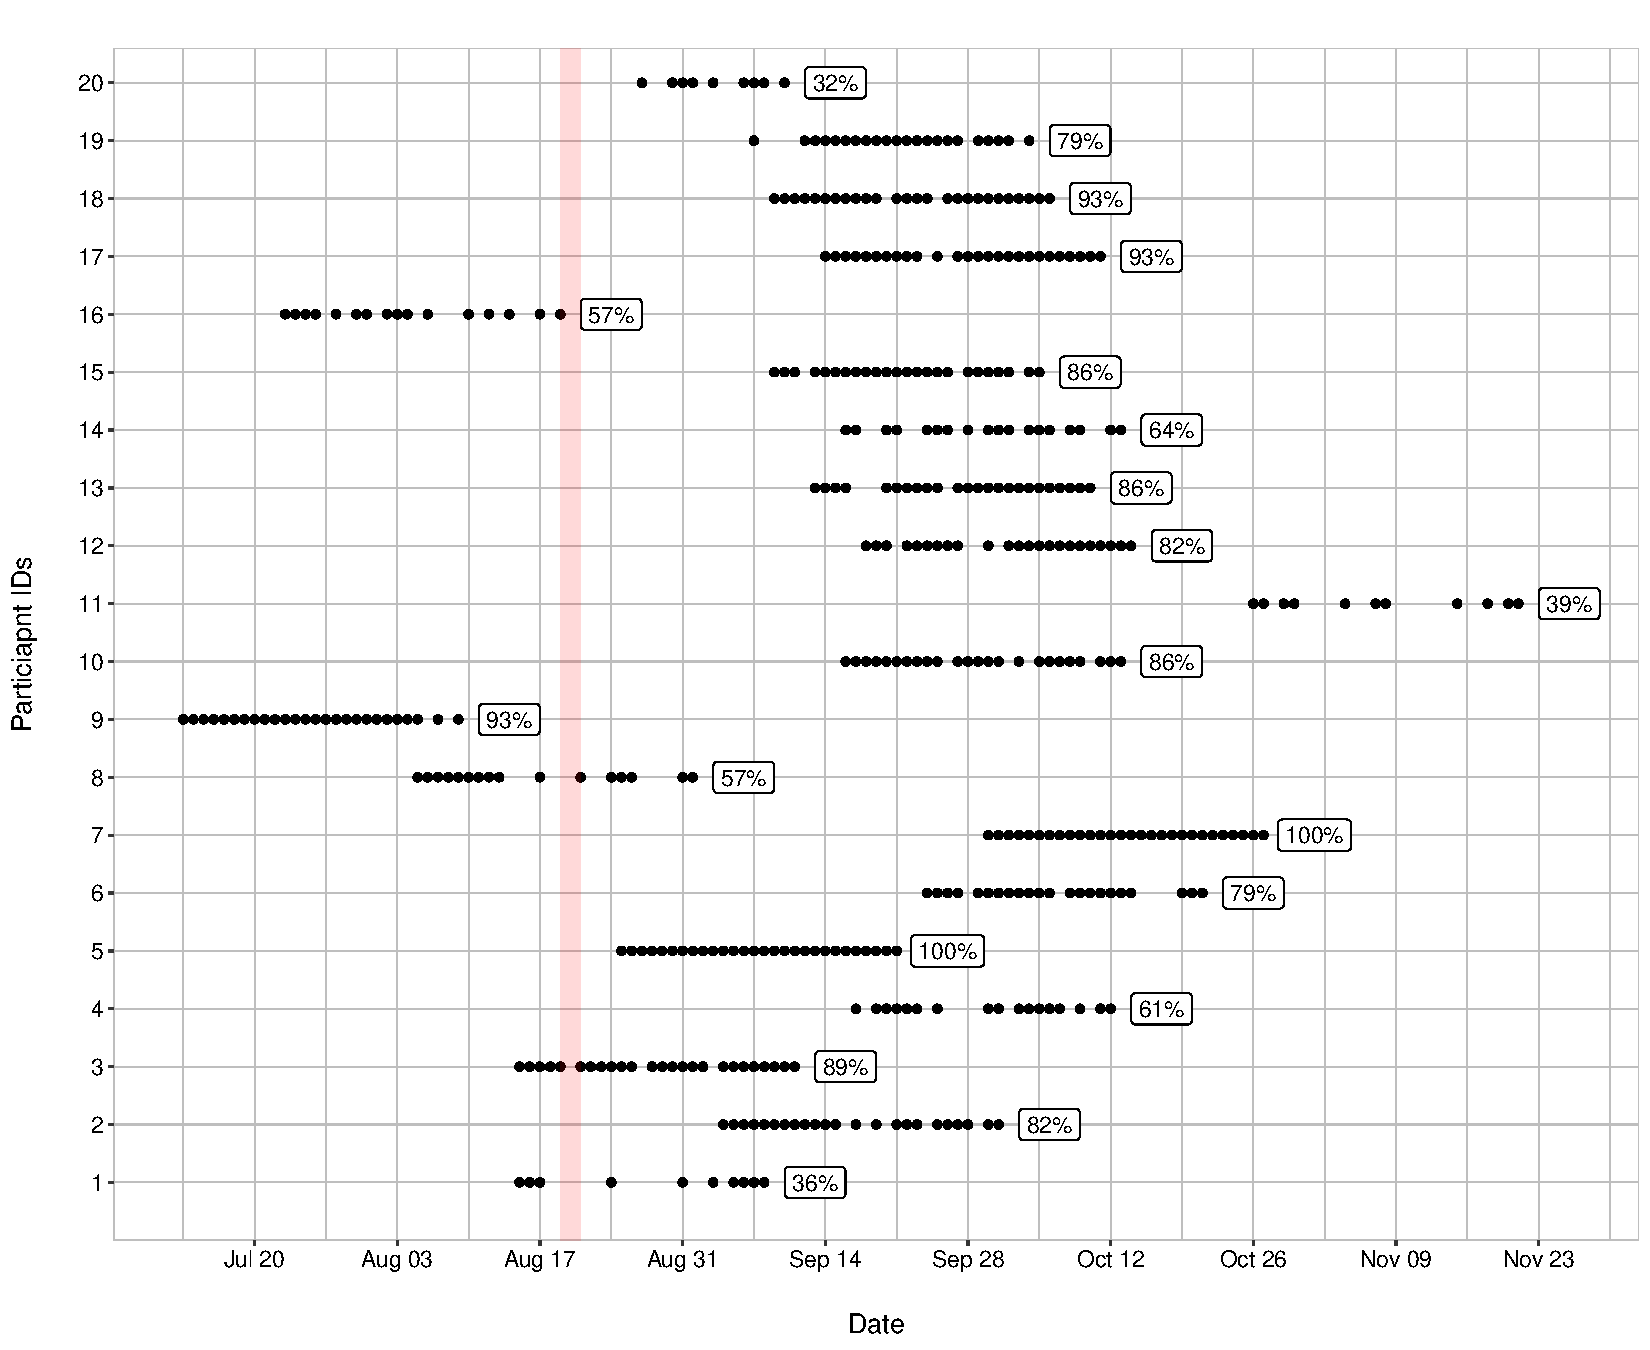
\includegraphics[clip, trim=0cm 0cm 0.15cm 0cm, width=\textwidth]{figures/engagement.pdf}
                \caption{Participants' engagement with the daily self-report of mental health and wellbeing via \acl{app}. Each dot represents an entry for the day. Annotations reflect each participant's rate of engagement calculated as the percentage of $28$ self-report sessions during the study. The red bar indicates Dialogflow's service outage on August 20th, 2020. Participants were not able to use \acl{app} on that day.}
                \label{fig:engagement}
                % \footnote{https://issuetracker.google.com/issues/165676621}
            \end{figure}
                
        During the study, $20,154$ words from $418$ daily open-ended self-reports were collected. On average, a participant's daily self-report contained $48.22$ ($\pm 30.48$ SD) words, lasting $46.96$ seconds ($\pm 31.33$ SD). The shortest self-report consisted of $4$ words while the longest contained $225$ words. Figure~\ref{fig:word-cloud} shows the words most frequently used by participants when responding to the open-ended questions eliciting expression of their emotional state. More than half ($59.33\%$) of participants engaged with the system during the evening hours of 18:00 to 21:00 as shown in Figure~\ref{fig:time_frequency}.
            
            \begin{figure}[h]
                \begin{minipage}{.48\textwidth}
                    \centering
                    %   l b r t
                    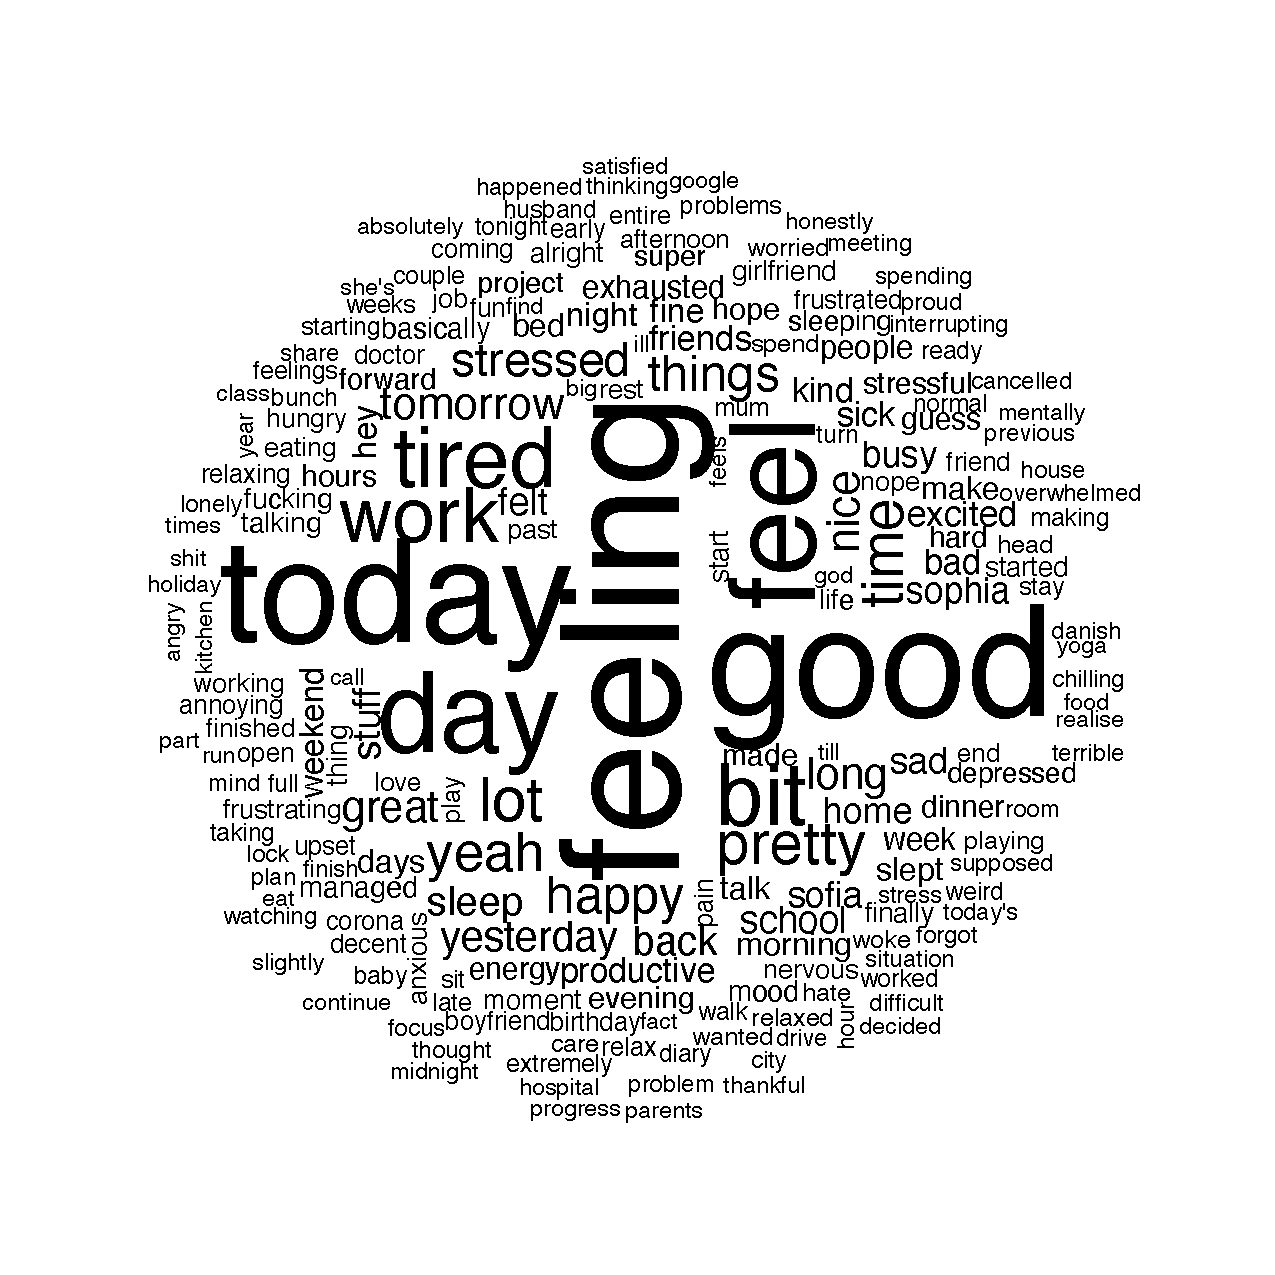
\includegraphics[clip, trim=2cm 2cm 2cm 1cm, width=\textwidth]{figures/word-cloud.pdf}
                    \caption{A word cloud generated from the participants' open-ended self-reports of their mental health and wellbeing}
                    \label{fig:word-cloud}
                \end{minipage}
                \hfill
                \begin{minipage}{.48\textwidth}
                    \centering
                    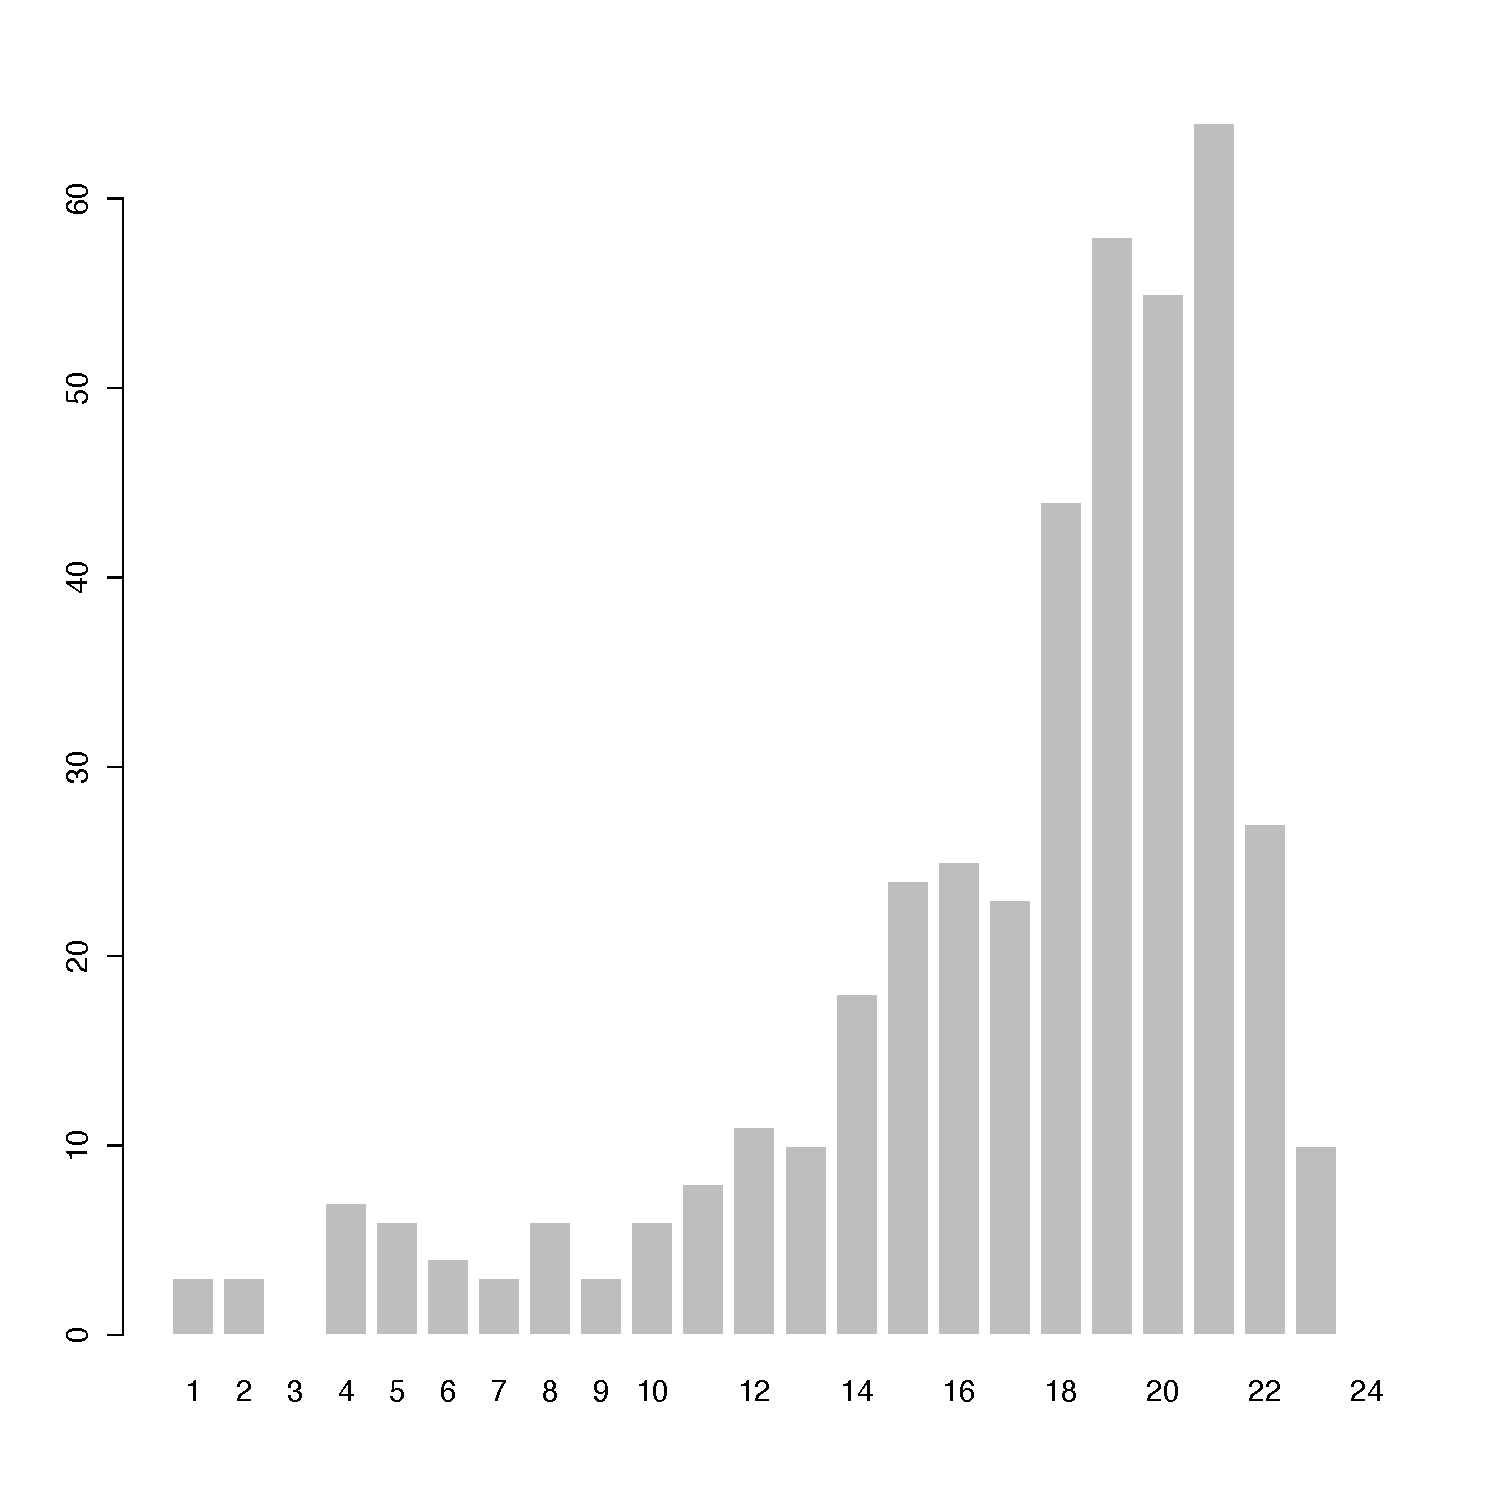
\includegraphics[trim=0cm 0cm 2cm 0cm, width=\textwidth]{figures/time_frequency.pdf}
                    \caption{Self-report frequency plotted against time of day. The x-axis represents the time of day in 24-hour format, and the y-axis self-report frequency.}
                    \label{fig:time_frequency}
                \end{minipage}%
            \end{figure}  
            
        % \subsubsection{Perceived User Experience}\label{sec:perceived_experience}
        As shown in Figure~\ref{fig:ueq-ci} participants' responses to the \ac{UEQ} questionnaire upon conclusion of the study reveal an overall positive impression of their self-report experience in terms of 
                attractiveness  ($U = 1.09, SD = 1.01 $), 
                perspicuity     ($U = 2.09, SD = 0.75 $), 
                efficiency      ($U = 0.98, SD = 0.77 $), 
                dependability   ($U = 0.74, SD = 0.84 $), 
                stimulation     ($U = 0.38, SD = 0.82 $), 
                and 
                novelty         ($U = 0.71, SD = 0.88 $). 

            \begin{figure}
                \centering
                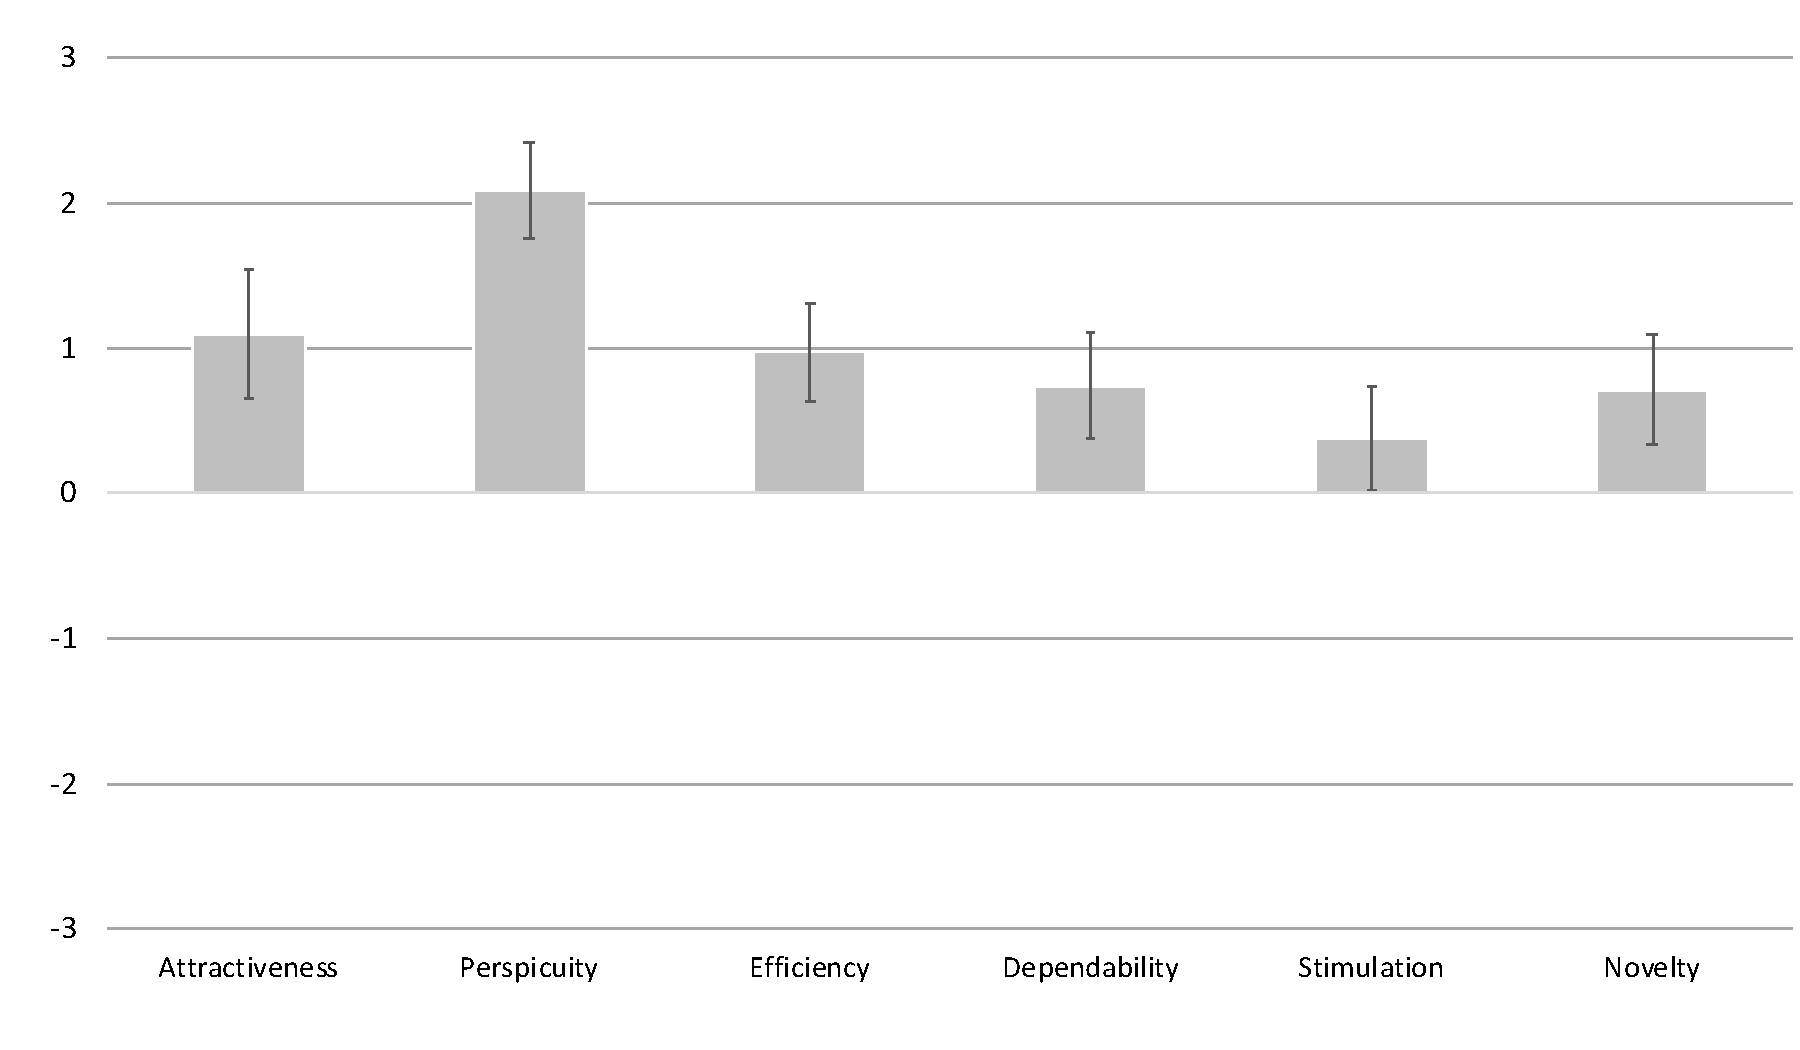
\includegraphics[width=\textwidth]{figures/ueq-ci.pdf}
                \caption{Participants' mean \ac{UEQ} score with respect to each dimension. Error bars reflect a $95\%$ confidence interval, the y-axis represents scores ranging from -3 (horribly bad) to +3 (extremely good), and the x-axis illustrates the six dimensions of the scale.}
                \label{fig:ueq-ci}
            \end{figure}
        
        These data serve as context for our thematic analysis of interviews conducted with participants following their engagement in this 4-week `in-the-wild' study; the primary findings of which we present next.
   
    % Users' experience as strongly shaped by actions taken to overcome the technological limitations of \ac{CA}s,
    % \subsection{Theme 1. A Good Experience can Enhance Engagement Despite Technical Limitations}
    \subsection{Theme 1. Engaging With \& Getting Around the Technology} % Overcoming Technological Limitations

        The theme we first discuss is one which informed all others, and stems from users' frequent comments to the need to get around the technology in order to fully engage with it. These comments relate for the most part not to choices made in the design of this particular \ac{CA} but to the more general limitations of commercially-available smart-speaker technology. These limitations undoubtedly had an impact on participants' self-report experiences, and yet the lengths to which participants went to overcome these limitations and maintain their engagement highlights the value participants saw in their use of the technology.
            
        % \subsubsection{An Efficient, Easy-To-Use and Attractive Medium of Self-Report} % UEQ related qualitative findings

        %     Many participants in this study pointed to the efficiency and convenience afforded by the smart speaker's hands-free experience as motivation for their sustained engagement with the agent;
            
        %         \begin{quote}
        %             \vspace{2mm}
        %             \textit{``I love it because it’s like an interface you talk directly to. It’s super easy to use. You don’t have to open your laptop and go to a specific page. I can just go home, open the door and talk to \acl{app}, super easy.''} [P1] 
        %             \vspace{2mm}
        %         \end{quote}
            
        %     Several participants also described how speech, as a more natural form of interaction, enabled them to express their emotions more freely and spontaneously compared to other means of self-report; \textit{``Speaking is much easier because you can just let the words flow and you don't have to think about it''} [P14]. The \ac{CA}'s tone of voice was likewise characterized by many participants as friendly, caring, and calming, resulting in a positive first impression in the context of their self-report experience; \textit{``My first impression was that I really liked her voice. She sounded very, very calming and caring''} [P7]. This was not a universal experience however, and other participants at times commented that \ac{CA}'s voice was robotic and lacked variation in tone and intonation.

        \subsubsection{Frustration, Rejection, Illusion \& Technical Limitations}
        
            Limitations described by participants include the \ac{CA}'s tendency to frequently interrupt and thereby impair their self-report experiences; due to both the \ac{CA}'s inability to recognize pauses between user utterances and the 12 second limit imposed on user responses. This would mean that participants were often interrupted in the middle of a sentence by the following question before they had completed their desired response. 
            
            % frustration / feeling of rejection / disconnect / value
            These experiences understandably proved frustrating for users, \textit{`I'm like `No bitch, you cut me off. So, shut up'\ldots''} [P9], and led to some participants quitting the conversation early; \textit{``Okay fine, that's it for today''} [P18]. Several participants compared their \ac{CA} interactions with a human-to-human conversation, and in turn expressed feelings of rejection following repeated interruptions and the inability to fully recount their emotional experience;
                
                \begin{quote}
                \vspace{2mm}
                    \textit{``I know it's not a human being. I know it's this little round little thing, but still it's like, I'm trying to be personal here and then you're interrupting me. It feels like a rejection.''} [P9]
                \vspace{2mm}
                \end{quote}
                
                \begin{quote}
                \vspace{2mm}
                    \textit{``I felt like a bit like when you talk with a friend, and they don't want to listen to you.''} [P8]
                \vspace{2mm}
                \end{quote}
                
            P8, in this example, relates their interrupted self-report experience to a conversation with a person who does not care, leading to a sense of disconnect. Similar accounts were shared by other participants who noted that it was important for them to feel listened to and cared for, despite their awareness that the \ac{CA} could not understand their emotions nor in reality `care' about what they shared.
            
                \begin{quote}
                \vspace{2mm}
                    \textit{``Of course, the software doesn't care. But, you want the illusion that it cares about you.''} [P5]
                \vspace{2mm}
                \end{quote}
            
            Many of these limitations of CA technologies are well-known and well-documented in prior literature (Section \ref{sec:ca_limitations}). What is most striking about participants' accounts as shared during this study however is the extent to which these technical limitations were recounted in emotional terms, and to which this reflects a desire by participants to relate to the technology. This theme is therefore furthermore supported by the strategies employed by participants to overcome these challenges.
  
        \subsubsection{Strategies to Overcome \ac{CA} Limitations}\label{sec:strategies_to_overcome}
        
            Participants described their development of a number of strategies to maintain their engagement;
            
            \paragraph{(i) Making Multiple Entries} % Beginning Again
        
                At the pre-study session, participants were given some insight into the limitations of the technology, and adding multiple entries was offered as a possible strategy for overcoming these challenges, should users encounter them. Only a small number of participants did adopt this strategy however; either accepting the technology's limitations and sympathizing with the CA, or interestingly, contrasting the \ac{CA}'s 12-second limitation with a human interlocutor's potentially limited capacity to listen to others;
                
                    \begin{quote}
                    \vspace{2mm}
                        \textit{``With my frustration, I took a deep breath and thought it’s just a technology. It’s in it’s starting phase - I let it do it’s thing.''} [P3]
                    \vspace{2mm}
                    \end{quote}
                    
                    \begin{quote}
                    \vspace{2mm}
                        \textit{``I guess that there's also like a limit to how, how long she can listen, like another person would also have.''} [P12]
                    \vspace{2mm}
                    \end{quote}
                
               Other participants noted that they did not find this a feasible strategy, commenting that they would lose their train of thought should they start a new session; \textit{``The problem is that you loose your momentum or train of thought when you're interrupted like that''} [P9]. P2, in contrast, compared their interactions to a human-to-human conversation and thought that it would be rude to ask \acl{app} to listen again: \textit{``when you're done talking to her and she is like `Thanks for sharing that. Have a nice day'\ldots it would feel rude to ask her again''}.

            \paragraph{(ii) Adapting One's Speech}
    
                Other participants adopted more active strategies. This included changing their natural speech patterns by stretching out their utterances, using filler words, and speaking faster or more briefly;
                
                    \begin{quote}
                    \vspace{2mm}
                        \textit{``I tried different tricks like for instance I tried to make some songs like `hmmm leeet meee thiiink' but it seems like my process was too slow for \acl{app}. So at one point, I started giving very short answers so I won’t be cut off yet could answer.''} [P1]
                    \vspace{2mm}
                    \end{quote}             
                
                Although considered effective, this approach was also certainly viewed by participants as a compromise;\textit{``My speech is a bit artificial, not very smooth, and didn't feel fluent. I had to change the way I talk to fit what \acl{app} can accept}'' [P8].
                    
            \paragraph{(iii) Preparing In Advance}
                    
                Another strategy spontaneously adopted by participants was to reflect in advance on what they desired to share with the \ac{CA}. P16 for example, recounted how they would divide their response into three parts to match the design of \acl{app}'s dialog flow:  
                
                    \begin{quote}
                    \vspace{2mm}
                        \textit{``I realized, okay two sentences for the first question, two sentences for the second question, and one sentence for the last question. Just five sentences overall.''} %[P16]
                    \vspace{2mm}
                    \end{quote}   
                
                Interestingly, some participants commented that this process of formulating their thoughts in advance in itself helped them to reflect on their day. P11 viewed this process as `meditative,' commenting, that \textit{``it helps you organize things in your head\ldots It's like `you time', you know, I believe it helps you clear your mind''}. P6 compared the experience to composing a concise diary entry which served to focus their reflections; \textit{``It's not just three pages of how I saw something nice and I had a nice cup of coffee\ldots It really is an emphasis on three things which really matter to me''}.
                
                Although for some participants such tactics led them to feel their responses were increasingly shallow, \textit{``She expects an answer in few seconds, so I'll be like, `tired', `decent', `not sure'. So in that sense, the answer might be a bit less thought out''} [P2], others showed a surprisingly significant willingness to adapt, at times expressed in overtly human terms;
            
                    \begin{quote}
                    \vspace{2mm}
                        \textit{``I started thinking about what I want to say before I called her up. Normally, when people talk about feelings, they need space and time for pauses. I knew my \acl{app} friend could not really do that. So we had to do it on her terms.''} [P7]
                    \vspace{2mm}
                    \end{quote}  
                
            A number of participants spoke to their increased capacity to adapt to the technology's limitations over time, despite the undoubted impact on their experience; \textit{``It was kind of hard in the beginning as she is really sensitive to pauses and doesn't give you any space to think. But my brain adapted that really quite quick''} [P7]. This willingness to adapt can only be interpreted in light of the value users associate with their interactions with the technology -- which, despite these limitations, appears to be closely related to their perceptions of the agent itself, as reflected in our second theme.

    \subsection{Theme 2. ``Sometimes All You Need is Someone Who Listens''}
    
        Engaging in the self-report of mental health and wellbeing by any means is an exercise in vulnerability. And many participants spoke to this effect, commenting how they would refrain from sharing their emotions even with close friends and family due to the social stigma attached to their illness. P7 and P14 noted the need to think about the potential repercussions of disclosure, listeners' reactions, as well as the potential for others to demonstrate disinterest in the subject, each of which demotivated their sharing of emotion;
    
            \begin{quote}
            \vspace{2mm}
                \textit{``You know, my dysphoria (\acs{PMDD}) often makes it so that I think that I'm a bother to people, like `it's really annoying to listen to you bitch'\ldots''} [P7]
            \vspace{2mm}
            \end{quote}  
    
        Another barrier to self-expression recounted by participants pertained to the potential for listeners to become pre-occupied with trying to understand their emotions in depth, requiring them to repeatedly explain what they are experiencing, when most of all they wished simply to be heard; \textit{``When you say you feel sad and empty, you don't really want the focus to be on describing how emptiness feels. You just want to say, `I'm feeling sad'\ldots''} [P6]. Strikingly, participants also frequently commented on their struggle with listeners' keen desire to `solve' their problems rather than listening to them. They explained that they usually do not require a solution to their problems, and due to the chronic nature of their conditions, often know how to cope with their situation and ongoing mental state; 
        
            \begin{quote}
            \vspace{2mm}
                \textit{``Sometimes all you need is someone who listens than have an answer\ldots because there's not necessarily anything to solve, you just need someone to share your thoughts and feelings so that you are not alone.''} [P2]
            \vspace{2mm}
            \end{quote}  
        
        This desire to be listened to, rather than to have their problems solved, goes some way towards explaining the value users saw in this particular \ac{CA} implementation, although interpretations and perceptions of \ac{CA} itself were strikingly diverse;
        
        \subsubsection{\ac{CA} as Good Listener}\label{sec:good_listener}
        
            Throughout the interviews, participants' comments echoed a desire for \textit{``emotional support instead of emotional counseling''} [P7], a role for which \acl{app} was often appropriated, as `someone' who made them feel heard. For many participants, therefore the \acl{app} was simply a good listener, who allowed them to express their emotions freely; 
            
                \begin{quote}
                \vspace{2mm}
                    \textit{``It sounds a bit stupid to say but I could say that I'm glad someone listens, except you know there isn't actually someone that listens. But it feels like it.''} [P2]
                \vspace{2mm}
                \end{quote} 
                
                \begin{quote}
                \vspace{2mm}
                    \textit{``She is a good listener. Sometimes a listener is exactly what you need in a situation like that.''} [P6]
                \vspace{2mm}
                \end{quote} 
                
            Participants valued the non-judgmental nature of conversations with \acl{app} which neither provided unwanted solutions nor meant that they had to worry about potential judgment and repercussions for sharing their feelings; \textit{``Since I knew \acl{app} doesn't mind, I felt it in some instances in a twisted way, I felt like she cared, like she was always there no matter how negative or positive I was feeling.''} [P7]. They furthermore appreciated \acl{app}'s compassionate feedback and mentioned that it would provide a sense of comfort and empathy when feeling depressed;
            
                \begin{quote}
                    \vspace{2mm}
                    \textit{``When you have a diagnosis like this, you know that only talking doesn't make it go away, but sometimes getting assurance `Okay, it's okay to feel, it's okay to experience what you experienced', that helps a lot.''} [P6]
                \vspace{2mm}
                \end{quote} 
            
        \subsubsection{\ac{CA} as Machine Companion} % Coach / Counsellor ?
            
            Other participants employed a vocabulary of companionship when describing \ac{CA}, associating the technology's value with its ability to fill a felt gap in their social interactions;
            
                \begin{quote}
                \vspace{2mm}
                    \textit{``When you are depressed, your social circle tends to restrain more and more. So, you’ve less opportunity to talk to someone. I felt like I was talking to someone even though \acl{app} is not very smart. Just because of this feeling, I think it is very useful for people with depression.''} [P1]
                \vspace{2mm}
                \end{quote} 
            
            For some participants, the \ac{CA}'s value, therefore stemmed from its constant availability; \textit{I do have friends to talk to. But a friend could be busy. When you need to talk it out, it’s in your reach even though it’s a machine'' } [P5]. Others spoke of the \ac{CA} as also more approachable and trustworthy --- a perception of the \ac{CA} as a harmless machine meaning that it could not turn against them no matter what they shared;
            
                \begin{quote}
                \vspace{2mm}
                    \textit{``I have massive trust issues. I grew up thinking that whoever you tell anything, they will use it against you. But, since I know that \acl{app} is a machine, she doesn't really think that much of herself and she's just there sitting on my table. That kind of makes it a little bit more approachable.''} [P7]
                \vspace{2mm}
                \end{quote} 

            And yet, for P4, talking to a \ac{CA} about their emotions could equally serve to make them feel lonely, given that the \ac{CA} could not `truly' understand their feelings; \textit{``Sometimes she made me feel a bit lonely, somehow, because you're just reminded that you're talking to a machine, who has no capacity to understand what you're actually feeling\ldots something that kind of tries to mimic a human being but it's not convincing''}.

        \subsubsection{\ac{CA} As Human} % Friend?
        
            Other participants went to greater lengths to personify the \ac{CA}, with both positive and negative implications and associations.

            % +ve personification
            Participants with positive perceptions of their self-report experiences tended to personify the \ac{CA} as a friend, therapist, or talking diary. Although noting their awareness that the \ac{CA} was not human, participants would often comment that the anthropomorphic characteristics of the \ac{CA} granted them the impression of a conversation with a person. P10, for example, who personified \acl{app} as a friend, commented \textit{``I think it's the whole, having a voice and having a name, I keep referring to it as her instead of it, even though I'm aware that it's a system and not a person''}. 
            
            P14 personified \acl{app} as an older friend and mentioned that although she could also be their age, \acl{app}'s voice made them think of someone older; \textit{``Its more like an older friend. I mean I'm also quite young, I'm 25 so maybe that's why? Maybe it's also the voice that reminds me of someone a bit older than I am''}. P15, on the other hand, viewed the \ac{CA} as a `talking diary' and compared their self-reporting practice to talking to their dog; \textit{``I compare \acl{app} to my dogs. Because a lot of the times, especially when I was growing up, if I was upset I went outside, sat down and talked to my dog who had no freaking clue what I was talking about, and it made me feel better''}.
            
            % -ve personification
            In contrast, participants with negative perceptions of their self-report experiences personified \acl{app} as an elderly woman, an uncaring friend, and a teenager trying to act grown-up. Referring to the \ac{CA}'s tendency to frequently interrupt her mid-sentence, P9 personified the \ac{CA} as a friend who does not care; \textit{``It's kind of like, you know, that friend who like sits with the phone when you try to talk about something deep, like `Okay fine, just say you don't want to listen to me'\ldots''}. Likewise, P3 personified the \ac{CA} as an impatient old lady, an impression informed by the 12-second response limitation and tone of voice; \textit{``\acl{app} is like a very impatient woman and she’s probably quite old. She’s very monotoned, there’s no variation''}.

            % Personification and self-reporting behavior
            These various personifications also shaped participants' responses to the agent, including their self-reporting behaviors. A positive personification of the \ac{CA} motivated P6 to find and share positive emotions even when negative ones were abundant; \textit{``You feel like, `Oh, I'm talking to someone and I don't just want to be negative. I want to say something positive'.''} Whereas, for P9, a negative perception of the agent led them to vent their frustrations directly to the device; \textit{``Sometimes I guess it took my emotions out. 
            %Sometimes I was yelling at her, telling her to fuck off. 
            It was probably not her causing the reaction, but because I was annoyed about something, and then I took it out on her. Sorry \acl{app}''}.
      
        \subsubsection{\ac{CA} As Blank Slate} % Null
     
            Finally, a number of participants spoke of emotional venting and self-talking as useful practices enabled by the smart speaker device. These accounts reflect interpretation of the \ac{CA} as a blank slate. P11 and P14 considered self-reporting via \ac{CA} a self-talking exercise, and stated that doing so helped them to clear their mind ~\cite{callicott2003effects,kendall1991guiding,treadwell1996self}. As P14 noted:
            
                \begin{quote}
                \vspace{2mm}
                    \textit{``Once you say stuff out loud, it just changes how you think about certain things\ldots when I have them in my head, it just sounds like they are super important. If I just talk out loud, then suddenly it becomes less important and I realize that they're just thoughts and they're not really like who I am.''} %[P14]
                \vspace{2mm}
                \end{quote} 
            
            Emotional venting has likewise been regarded as an effective means of finding relief by releasing strong or repressed emotions~\cite{bennett1991irrationality, tonnaer2020explosive, leslie2008boxing}, a practice on which P8 commented;
            
                \begin{quote}
                \vspace{2mm}
                    \textit{``I almost see it as, you know, when you get super upset, you go out and scream, you go very far away and you just scream at the wind, cows or whatever. And you know that you're never going to get anything back, like, no one is going to respond to you, but it feels good to just express.''} %[P8]
                \vspace{2mm}
                \end{quote} 
            
            These various perceptions of \acl{app} suggest the value of different framings and implementations of mental heath agents, and multiple paths forward for their future design for varied yet valuable purposes. The prevalence of personification in itself furthermore underlined the extent to which participants perceived self-report as a socially-contingent practice.        

    \subsection{Theme 3. Self (Report) is Social}
    
        While all forms of self-report, and indeed human behavior, are to one degree or another socially-contingent in nature, participants' experiences of \acl{app} in particular revealed a diverse variety of social associations. Many of these accounts stem, at least in part from the spoken nature of the interaction itself, and in turn its more open nature.

        \subsubsection{A Private Practice Rendered Social} % Social influence in self-reports
            
            Eight of the twenty ($40\%$) participants in this study mentioned that they engaged with \ac{CA} in an open environment (e.g., a co-living space) where the presence of others' was likely to have an effect. And yet this was not the only way in which social considerations were seen to manifest. The choice of a number of participants to make their self-reporting a private practice was also informed by their social circle's perception of the \ac{CA}, as well as their relationships to their loved ones.
            
            The self-report of mental health and well-being is most typically a private practice, due at least in part to the social stigma attached to many mental health conditions, and the potential lack of privacy when engaging with a \ac{CA} therefore creates a unique self-reporting context. Participants P17 and P20 commented that it felt `weird' and `awkward' to talk to \acl{app} when other family members were around; \textit{``It felt a bit weird talking to a speaker and was especially weird when my husband was home. It was unnatural in general but especially when I had someone else listening at the same time''} [P17]. For P4, this experience was awkward because it created confusion when their partner did not know that they were talking to the \ac{CA}:
            
                \begin{quote}
                \vspace{2mm}
                    \textit{``Talking to \acl{app} is little awkward because because if my boyfriend wasn't aware of what I was doing, He's like, `What? `Do you want something from me?'\ldots like `No no. I'm talking to the device'. Yeah, `I'm talking to this other thing in our house'.''} %[P4]
                \vspace{2mm}
                \end{quote} 
            
            P6 shared that although it was also strange for them to talk to \acl{app} initially, it became natural due to their partner's support -- serving as an interesting example of the implicit value of such a technology in providing an opportunity for others to demonstrate care;
            
                \begin{quote}
                \vspace{2mm}
                    \textit{``At first, I felt like this is something personal. Like, this is something I should hide, like a diary under the pillow or something. But, well first of all, my husband has been really supportive and he is like, `Remember your \acl{app}, Remember to talk to her'. So it became more natural to talk to her.''} %[P6]                
                \vspace{2mm}
                \end{quote} 
            
            Of course, reporting practices varied among participants, as intended by a study designed to allow users to appropriate the technology as they saw fit. P11 noted that they were comfortable sharing their feelings in the presence of others, \textit{``I don't mind\ldots sharing these things with my friends, or anyone to be honest''}, whereas P3 commented that they refrained entirely from self-reporting when friends were around; \textit{``I’d have friends over so during those times, I didn’t log a diary -- You don’t want to let everyone know about deep personal life.''}
  
        \subsubsection{A New Member of the Social Circle} % Social perception of \ac{CA} self-reports
        
            Other participants went further, and spoke of \acl{app} as entering into their social circle. A number of participants commented that their social circle held a positive view of the \ac{CA} and supported the idea of talking to \acl{app} about their emotions. P1's partner, for example, told P1 that \ac{app} could help them when they were feeling down; \textit{``My boyfriend told me that maybe I should use \acl{app} when I was down. He told me that I shouldn’t be closing myself to the world, I should be talking. He said it might be useful.''}. 
            
            P6 spoke openly about the study with friends and family, and described their friends as very curious about the technology, which quickly became a topic of conversation in their daily lives;
            
                \begin{quote}
                \vspace{2mm}
                    \textit{``I remember a friend who said `so how's it going with \acl{app}?', and they started joking and like `So when is she going to tell you about her'? It's quite interesting how she became this little person in my life somehow''} %[P6]          
                \vspace{2mm}
                \end{quote} 
            
            P6 continued that their father was equally excited about the technology and shared that he had in turn also expressed an interest in purchasing a smart-speaker, as a potential means of addressing loneliness. However, they also wondered whether their father would be able to set up the device;
            
                \begin{quote}
                \vspace{2mm}
                    \textit{``I talked to my dad, he was really interested. 
                    He's like how does someone put a voice in this tiny box? like he doesn't understand it's just code and such. I asked him if you would buy something like this and he said yeah he probably would because he's also alone a lot of the times. But he also said, `if I have to use it with apps and phones, I can't figure out how to do with them'\ldots ''} %[P6]
                \vspace{2mm}
                \end{quote} 
            
            P18's friends similarly thought that \acl{app} was `cool' and expressed its potential to support mental health and wellbeing. Their partner commented however that, although such a system could help those particularly isolated, it would not be able to replace a more human connection;
            
                \begin{quote}
                \vspace{2mm}
                    \textit{``My boyfriend is a therapist himself and he said that, that might be smart. It could do something for very very very lonely people. They could feel like, `Well, there's someone who is interested in my day'. But we also talked about like we don't think an artificial intelligence can ever replace of a real life person''} %[P18]
                \vspace{2mm}
                \end{quote} 
            
        \subsubsection{An Influence On Close Personal Relationships} % Self-reporting via \ac{CA} and social relationships
        
            Finally, and perhaps most surprisingly, a number of participants spoke of the influence of \acl{app} on their intimate and personal relationships. Several noted that openly describing their emotions to the \ac{CA} also led to conversations with their partners, and served to strengthen their relationships.

            P4 commented that after hearing her response to the fortnightly \ac{WHO-5} questionnaire, her partner realized for the first time just how she had been feeling during those two weeks; \textit{''When he heard me responding to \acl{app}, he was like, `oh so this week is that shit? I didn't know'\ldots''}, creating a `different situation', \textit{``an intervention in your life where you're like, so this is how you're actually feeling''} despite the fact that \textit{``of course, we see each other every day, we live together. I do tell him if I'm tired or mad or whatever and try to keep him in the loop about my moods. But it's also just like sometimes you're not aware of it yourself''}.
            
            This potential of the technology to shape the social fabric of a household was reflected in several other participants' comments. P6 mentioned that their mental condition could make it hard for them to explain exactly how they are feeling, and that their tone of voice when speaking to \acl{app} therefore became the medium by which their significant other could best understand how they are actually feeling;
            
                \begin{quote}
                \vspace{2mm}
                    \textit{``Sometimes I will talk to her and not like I said anything specific but more like he [P6' husband] could feel from, how I was talking to \acl{app}, my tone of voice. Some days he would peek his head in and be like, `Do you want to talk about anything?. Are you okay?', because I can be feeling extremely bad, but I'll look Okay.''}
                \vspace{2mm}
                \end{quote} 

            P14 spoke of a moment of realization during which her and her partner noticed that although they talked about their daily activities, these conversations did not necessarily reflect their feelings. 
            
                \begin{quote}
                \vspace{2mm}
                    \textit{``My boyfriend does not share his emotions very often, neither do I. 
                    %You always ask like `How was your day?' but then it's always a bit vague. 
                    So sometimes when I was talking to \acl{app} and he (P14's boyfriend) noticed that I had some different feelings which he wasn't aware of. It was quite good in that way. Now we are speaking more about feelings. 
                    %Now we ask `How are you feeling today?' and it's not only good but then 
                    We also have more details about how it is going. 
                    %I think it's very important.
                    ''}
                \vspace{2mm}
                \end{quote} 
                
            Many participants' comments therefore reflected an open and welcoming attitude towards \acl{app}. And yet, this did not preclude attention to questions of privacy and security, as our final theme highlights.

    \subsection{Theme 4. Personal Privacy \& Data Security}\label{sec:privacy}
    
        In line with prior research~\cite{lau2018alexa}, participants' engagement in self-report was also shaped by their perceptions of personal privacy and data security. Although open to interpretation as pragmatic in nature, the implications of these concerns were not straightforward, as this theme highlights.   
        
        \subsubsection{Away From Prying Eyes \& Ears}\label{sec:eavesdropping} % Eavesdropping
        
            A number of participants recounted privacy concerns stemming from their own and their wider social circle's perception of the technology. The concern most-often shared related to the potential for the smart-speaker device to continuously listen and record conversations, even when not activated. In order to protect their privacy, participants described either turning off the smart speaker's mic or unplugging the smart speaker entirely. Participants P12 and P14, for example, both commented on the potential of the technology itself to serve as a source of anxiety, and subsequently chose to keep the microphone off at all times, only turning it on when speaking to \acl{app}: \textit{``I felt a bit paranoid so I was like turning the speaker off''} [P12].
   
            A small number of participants commented on their resignation from engagement with the challenge of navigating many questions of privacy, due to a perception that it was broadly impossible to avoid pervasive collection of their data. P16, for example, mentioned that they did not mind sharing their data as long as they got something in return: \textit{``I'm not really concerned about privacy because I cannot stop them (tech companies) from collecting the data. But if I'm sharing something, I need something in return. For example, I really like that every month Google sends you  a timeline and gives you how many kilometers you have walked''}.
            
        \subsubsection{Hands Off Our Data} % Data security
            
            In addition to their concerns regarding potential eavesdropping, participants expressed an interest in knowing and closely controlling how their data would be handled, citing understandable fears that their data might be shared with a third party or become publicly available. 
            
            Although appropriate limitations on the use of patients' data were carefully explained both in-person and within participant materials, these privacy concerns understandably had an impact on certain participants' self-reporting practices. P9 commented that they \textit{``probably held back, a great deal. Because of the whole, I know that it's not ending up in cyberspace for anyone to see but there's still that thought that is a bit more out of my control than if I have it in a physical diary''}. Despite describing herself as an open book, P18 also commented that knowledge of the research team's access to her transcripts led her to refrain from fully recounting her mental states, \textit{``I knew that you would get the transcript of what I told her. Now, I'm not really a private person and I'm pretty much an open book, but I did refrain from saying stuff that I would have said if I knew you wouldn't be able to read it''}.
                      
            These concerns are not new, yet are particularly important to consider, and of particular ethical significance, in the lives of this population group, whose involvement in this study and engagement with this technology consisted of a vulnerable exercise requiring high levels of social trust and personal courage. 
        
    % \subsection{Theme 5. Action Items to Improve Conversational Interaction for Mental Health Self-Report }\label{theme:design_recommendations}
    \subsection{Theme 5. Designing for Conversation \& Reflection}\label{theme:design_recommendations}
    
        Many participants spoke of the value of the technology as allowing them to fully express their emotions, and yet also as one of the ways in which the system was currently most limited. Additionally, they highlighted the potential need to reflect on their self-reported data and discussed ways to enable this.
        
        \subsubsection{Designing for Conversation}\label{sec:improve_design}
            
            Participants made several design recommendations to improve the \ac{CA}'s conversational skill, and allow users to express their emotions more fully.
            
            \paragraph{(i) Varying More Often}
            
                Participants recommended incorporating greater variation in questions, including voice characteristics (e.g. tone and intonation), and randomizing their presentation more often so that the questions did not feel repetitive;\textit{``No one's going to ask you the same kind of question in the same way with the same intonation every time. So having a few different questions and rotating them would be better''} [P18]. In contrast however, P6 noted that the repetitiveness of certain questions provided consistency in interaction which they found important; \textit{``What's really important when you suffer from a condition like schizophrenia is consistency \ldots And in that regard, I almost find a sort of comfort in \acl{app}. She is like an anchor, which you can use to ground yourself, because she always says the same thing''}.
            
                Participants perceived the fortnightly \ac{WHO-5} questionnaire as a useful addition of variety to the daily open-ended questions; \textit{``I was happy when those questionnaires came up - it was something different at least''} [P5], and several suggested also adding more discrete questions to the conversation design; \textit{``She could toss in some of that once in a while that wouldn't actually be bad''} [P4]. While many agreed that closed-ended questions can be more efficiently answered, P9 and P10 also interestingly noted that responding to the discrete questions according to a pre-defined scale made them feel more like study subjects; \textit{``You feel a bit more like a study subjects like okay `How do you feel from 1 to 10?', it's like `okay 1\ldots 5\ldots 3'\ldots''} [P9]. 
                
            \paragraph{(ii) Probing Further}
                
                Participants suggested probing their responses further to engage them in a more `natural' conversation. They stressed that the \ac{CA} does not need to understand everything but could employ strategies to support a richer conversation. P20 provided an example; \textit{``For e.g., If I say, `It was a very busy day, very overwhelming', then she could ask like, `How did you deal with that?' `How could you improve?', So it’d be best if there was an \ac{AI} which could pull out some key words and follow up on the basis of those keywords''}.

            \paragraph{(iii) Guiding More}
            
                Many participants also suggested alternate conversation designs. P18 commented, for example, that when depressed, they would tend to have negative thoughts all the time, and would appreciate a conversation that encourages them to talk about something positive in their lives; \textit{``She could ask me like, `Can you tell me a positive thing that happened to you today?' I can always tell you about bad things happening in my day. It would be better if I was turned away from that a little bit''} [P18]. P15 shared similar views but argued that the conversation should delve into both positive and negative emotions, including the reasons behind those emotions. P12 and P19 likewise advocated enabling users to select the topic of the conversation, envisioning a set of topics from which users could choose, allowing users to lead the conversation and reflect more deeply on their emotions; \textit{``If it had a certain set of questions for different topics that would help people reflect a lot more and having to be the one leading the story through the entire way''} [P19].

        \subsubsection{Designing for Reflection}\label{sec:reflection}
        
            The practice of reporting entails reflection - a point a number of participants highlighted - and the design of a self-report experience might therefore equally be construed as structuring a practice of reflection. Participants' comments for improvements in turn pertained not only to the current conversational design but also to the potential to support further reflection on their own reported data. Many participants discussed the need for a visual tool as a mobile or web app displaying the trend of their emotional wellbeing for self-reflection, arguing that it would be the easiest means of searching and examining their information.
                   
            Others however, also raised the possibility of adapting the voice interface to support reflection. P14, for example, reflected on their use of a mobile app for this purpose and mentioned that they often ignored the data shown by the app. Via verbal reflection, they stated, it would feel more like confronting a problem, which they would find more meaningful than visually examining their data; \textit{``If someone is telling me like `Hey man, I've noticed that the last couple of days you have been really stressed out, is there anything wrong?' or `What's going on?'. It's more confronting\ldots and I think that gives me way more like meaning than if I just see that in the app''}.
            
            For P15, reflecting via \ac{CA} could also provide value by granting them more scope to disagree with advice provided. Compared to the potential for confrontation with friends, family, and therapist, they felt this approach could better support behavior change; \textit{``I would be way more likely to listen to a machine because even if it tells me something like a recommendation or tells me what to do, if I don't want to do it, I'm not gonna do it''}. Participants discussed different ways in which the \ac{CA} could present data verbally for users to reflect upon. They debated whether the \ac{CA} should automatically announce the data every session or on-demand. Those who supported automated voicing of the data recommended that the information should be announced casually at the end of the session. Others cautioned that the idea of presenting the data without users' request could prove intrusive depending upon the user's mental state; \textit{``It's kind of a double edged sword, because it can be intrusive if you don't want it. If you don't want any feedback, and then \acl{app} tells you, `oh it's been really bad the past three weeks.' That's the last thing that you want to hear''} [P8].
            
    We conclude this paper with further reflection on these themes and their implications for design.

% UNUSED NOTES
% \subsection{Summary of the Qualitative Findings}\label{sec:enablers_barriers}
% elow, we summarize the key findings from our thematic analysis of the interviews.
% Table~\ref{tab:theme_summary} summarizes the five major themes from our qualitative analysis of the interview data.
% and outlines users' perceptions of \ac{CA}s for the self-report of mental health, including enablers and barriers to their use.
% \begin{itemize}
% \item\textbf{\ac{CA} as an engaging medium for the self-report of mental health and wellbeing.} Overall, participants in this study perceived \ac{CA} as an efficient, easy to use and attractive medium self-report despite its technical limitations. Although some participants expressed their self-reporting experience via \ac{CA} as frustrating and feeling of rejection, many appropriated the system by applying tactics such as making multiple entries, adapting one's speech, and preparing in advance.
% \item\textbf{``Sometimes All You Need is Someone Who Listens.''} Due to the social stigma attached to mental illnesses, many participants in this study expressed that they refrained from sharing their emotions even to close members of their social circle. Their desire to be heard was perceived as fulfilled by \acl{app}, which led them to personify the \ac{CA} as a good listener, companion, and blank slate.
% \item\textbf{Self (Report) is Social.} Participants shared the personal and interpersonal effects of using the \ac{CA} for the self-report of mental health and wellbeing. For participants living in co-living spaces, the typically private practice of self-report became social. Some described the \ac{CA} as a new member of their social circle, while others mentioned its positive influence on their close personal relationships.
% \item\textbf{Personal Privacy \& Data Security.} Participants were mostly concerned about the possibility of smart speakers eavesdropping even when they are not activated. They either turned off the smart speakers' mic or unplugged the device entirely to protect their privacy. Participants expressed that the transparency about the data practices in the study enabled them to take necessary actions to use the system at their own discretion.
% \item\textbf{ Participants’ Design Recommendations.} Based on their self-reporting experiences via \acl{app}, participants recommended improving \ac{CA}'s conversational skills by varying the questions more often, probing on their responses and guiding the conversation, and providing space for reflecting on their self-reported data.
% \end{itemize}
% \begin{table}[h]
    \footnotesize
    \centering
    \caption{Summary of the themes as users' perceptions, enablers and barriers of using \ac{CA}s for mental health self-report}
    
    \begin{tabular}{p{3.20cm} p{4.65cm} p{4.65cm}}
        \toprule
        \textbf{Themes (Perceptions)}	& \textbf{Enablers}	& \textbf{Barriers}\\
        \midrule
            
            \begin{itemize}[leftmargin=0em]
                \item[] 1. Engaging With \& Getting Around the Technology
            \end{itemize}   
        & 
            \begin{itemize}[leftmargin=1em]
                \item Speech as an efficient and easy medium of self-report
                \item \ac{CA}'s friendly, caring and calming voice
                % benefit = burden-free self-report
            \end{itemize}
        &  
            \begin{itemize}[leftmargin=1em]
                \item \ac{CA}'s technical limitation constraining the length of open-ended self-report
                % risk = adding up unwanted stress    
                \item Robotic voice of \ac{CA} due to lack of variation in its tone and intonation
                % risk = disengagement
            \end{itemize}\\ \rowcolor[gray]{.95}  
            

            
            \begin{itemize}[leftmargin=0em]
                \item[] 2. ``Someone'' (or something) ``who listens''
            \end{itemize}
        & 
            \begin{itemize}[leftmargin=1em]
                \item \ac{CA}'s anthropomorphic characteristics
                \item \ac{CA}'s compassionate feedback 
                \item Continuous availability 
                % benefit = Repercussion-free and non-judgmental venting of emotions
                % benefit = \ac{CA} as a companion
                % benefit = providing sense of comfort and empathy
            \end{itemize}
        &  
            \begin{itemize}[leftmargin=1em]
                \item \ac{CA}'s inability to understand users' feelings
                % risk = Feeling of loneliness because \ac{CA} is just a machine
                % risk = \item Negative personification leading to vent their frustration on \ac{CA}
            \end{itemize} \\
            

            
            \begin{itemize}[leftmargin=0em]
                \item[] 3. Self (Report) is Social
            \end{itemize}
        & 
            \begin{itemize}[leftmargin=1em]
                \item Support from users' social circle
                % benefit = \ac{CA} as a medium to share emotions with the loved ones
                % benefit = Positive influence on users' intimate and personal relationships
            \end{itemize}
        &  
            \begin{itemize}[leftmargin=1em]
                \item Users' social situation
                % risks = Talking about feelings without privacy is strange, weird and awkward
                % risks =  Talking to \ac{CA} in co-living spaces creates confusion
            \end{itemize} \\ \rowcolor[gray]{.95}  
            
            
    
            
            \begin{itemize}[leftmargin=0em]
                \item[] 4. Personal privacy and data security
            \end{itemize}
        & 
            \begin{itemize}[leftmargin=1em]
              \item Privacy resignation 
              \item Ethics and regulation
            \end{itemize}
        &  
            \begin{itemize}[leftmargin=1em]
                \item Users' privacy (eavesdropping) concerns
                \item Distrust of \ac{CA} data security
                % risk = Paranoia and anxiety due to the concerns
                % risk = data quality (they held back on their self-report)
            \end{itemize} \\ 
            
            
            \begin{itemize}[leftmargin=0em]
                \item[] 5. Need for improving conversational design and space for reflection
            \end{itemize}
        & 
            \begin{itemize}[leftmargin=1em]
              \item Desire to express their emotions fully
              \item Desire for Self-reflection
            \end{itemize}
        &  
            \begin{itemize}[leftmargin=1em]
                \item Repetitive and static conversation
                \item Lack of self-reflection mechanism in \acl{app}
                % risk =  Verbal reflection potentially intrusive
            \end{itemize} \\
            
        
        % 3. Self-report as a social practice   &   Improved relationship with the loved ones   &    Privacy and Social Stigma  \\
        % 4. Personal privacy and data security &   --    & Trust \\
        \bottomrule
    \end{tabular}
    \label{tab:theme_summary}
\end{table}

% ----UEQ NOTES----:
% Attractiveness = Annoying-Enjoyable, Good - Bad, Unlikable - Pleasing, Unpleasant - Pleasant, Attractive - Unattractive, Friendly - Unfriendly
% Perspicuity = Not understandable-Understandable, Easy to learn - Difficult to learn, Complicated - Easy, Clear - Confusing
% Efficiency = Fast - Slow, Inefficient - Efficient, Impractical - Practical, Organized - Cluttered
% dependability = Unpredictable - Predictable, Obstructive - Supportive, Secure - Not Secure, Meets expectations - Does not meet expectations
% stimulation = Valuable - Inferior, Boring - Exciting, Not Interesting - Interesting, Motivating - Demotivating
% novelty = Creative - Dull, Inventive - Conventional, Usual - Leading edge, Conservative - Innovative
% ----UEQ NOTES----
% pragmatic quality = Perspicuity, Efficiency, Dependability
% hedonic quality = Stimulation, Originality 
% attractiveness = attractiveness
% Left flushed comments are notes
% All $20$ participants completed the study and were compensated with a Google Nest device.
% We present our findings from a 
% quantitative data: adherence and UEQ
% first, we report on the quantitative findings of the study which includes participant's adherence to the study protocol and perceived experience as measured by their response to the \ac{UEQ} questionnaire. 
% quotes and themes that represent/discuss the findings
% We then present the our findings from the thematic analysis of the interviews which shows that 
% users' self-reporting experience is strongly shaped by
%     \ac{CA} features and limitations,
%     \ac{CA} affordances,
%     social situation, and
%     their privacy perceptions.
%  We discuss these findings in following 4 themes:
%   (i) users' tactics to overcome \ac{CA} limitations to self-reports,
%   (ii) ``Sometimes all you need is someone who listens'',
%   (iii) social influence in user' self-reporting behavior and relationships ,
%   (iv) users’ privacy perceptions and security concerns.
% regarding the factors influencing self-reports of mental health and wellbeing via 
% Factors which shape user experience, behavior and perception.
% illustrates the summary of the participant's adherence to daily self-reports during the study period. 
% and indicates participant's acceptance of \ac{CA} for self-reports. 
% Tactics to overcome \ac{CA} limitations to support self-reports \ac{CA} features and limitations surfaced as the most prominent factor that affected users' self-report experiences.
% limitations: don't understand user pausing and 12 sec limitation         
% Because they were not able to share their thoughts completely, P3 questioned the value of self-reporting via \ac{CA}: \textit{``She'll cut you off anyway. There's no point to talking to someone if you're not allowed to complete your thoughts''}. 
% \textit{``When it cut me off, I was little annoyed, I didn't have so much patience with her. I was like, Okay fine, that's it for today''} [P18].     
% tactics 
% \subsubsubsection{Changing the natural way of talking. }
% \subsubsubsection{Formulating self-reports beforehand. }
% desire to talk longer
% While participants were able to alleviate \ac{CA} limitations to self-report about their mental health and wellbeing, they expressed their desire to be able to talk for more than 12 seconds and wished that \ac{CA} did not interrupt the conversation by cutting them off mid-sentence, allowing them to reflect on their day and fully express their state of mind.        
% \textit{``I think it would make more sense if I could speak at length, and she didn't cut me off''} [P4].
% Others explained that limitations affected their self-reporting experience mainly at the beginning of the study they were able to adapt to the \ac{CA} constraints and eventually learned to talk to the \ac{CA}.
% Therefore, they valued being heard than having their problems solved. 
% Why its difficult for them to share feelings?
% Why they don't feel heard?        
% \subsubsection{Barriers to share emotions}
% explanation
% unwanted solution.       
% Participants described that it is generally challenging for them to communicate their feelings to others therefore they often withdrew themselves from sharing their feelings. - open door for CA
% Participants widely shared their perceived affordances of \ac{CA} such as (i) good listener (ii) companion and (iii) tool for emotional venting.
% no judgment, repercussion
% Participants agreed that during their depressive state all they want is someone who listens and they found \ac{CA} a good listener.
% often personified the \ac{CA} by comparing their experience talking to \ac{CA} with their prior experiences and discussed \ac{CA}'s potential as a companion. % \textit{``When I have schizophrenic thoughts, I get intrusive thoughts a lot. And they are really unpleasant and people ask me about it but it's not like you want to tell someone `Oh it's just that I'm thinking about smacking in the head of a person or something'. It is a thing with \acl{app} which I think is really nice because I have a lot of things I don't really feel like I can talk that naturally about, even with friends and family. I would think there's only like one or two persons I could to talk to about these things the same way I can just sit down and tell \acl{app}''} [P6].
% In contrast, participants with frustrating self-reporting experience, P9 for example, often lashed out their frustration on \ac{CA}:
% \textit{``If you have access to some of my logs, you will actually see that some of the logs are basically just me saying `Fuck you, \acl{app}'.}
% Most participants personified the \ac{CA} in different forms. Participants' personification of \ac{CA} reflected their self-reporting experience and how they perceived \ac{CA}'s characteristics such as voice and name.
% \subsubsection{Emotional venting and self-talking}
% Social influence in user' self-reporting behavior and relationships
% Unlike traditional forms of self-reports such as diary and mobile apps, which grant different privacy levels, self-reporting via \ac{CA} using a smart speaker is more open to the surroundings. 
% influencing users' self-reporting behaviors and experiences.
% Felt Weird
% P17 mentioned that it was unnatural to talk about their feelings when someone else is listening.
% P20 said that it was not only awkward to them but also to the listeners:
% \textit{``I think they could feel how awkward I felt about it a little bit. And it was interesting that they could listen to me speaking to \acl{app}, and they had a follow up question and asked, `Why did you say that?'''}
% creates confusion
% Weird at beginning but their partner was supportive           
% P20 shared similar realization, quoting,
% \textit{When \acl{app} asked me,`How are you feeling today?' - I listed what happened during the day. Then my loved ones would tell me, `She’s asking how you felt, not what you did!'. Then, I realized that’s actually a good distinction. There was a moment when I realized even in real life, I’m not good at telling people how I’m feeling. When someone asks me that question, I just assume that they’re asking a summary of what I’ve done. So, it’s an interesting question \acl{app}’s asking.}
% Facilitates conversation about your mental state with your significant other
% P14 mentioned that neither them or their partner shared their emotions with each other. However, their partner's realization that they had different feelings than what they were aware of, encouraged them to talk more about their feelings. By doing so, they mentioned that they had better understanding of each other. % Privacy-Seeking Behavior
% \textit{A lot of my friends are talking about like that it listens to whatever you're saying. I felt a bit paranoid so I was like turning the speaker off} [P12].
% likewise, P14, unplugged the speaker except to talk to \acl{app}:
% \textit{``He (P14's boyfriend) didn't like it when it was there when we would go to bed for example. It might overhear us when we were talking or something like that''}.
% P14 mentioned that they later placed the smart speaker away from their bedroom and kept it plugged in. They added that their fear of privacy declined as they got used to it: 
% \textit{``I was quite afraid about the security thing but the more I used it, the more I feel comfortable using it.''}
% Both participants also discussed the relationship between their mental state and their privacy concerns. P14, for example, reflected on the potential for the technology 
% \textit{``This may be also where anxiety comes from. It just gets me freaked out that it's next to my bed...when we go to bed, it might overhear us''}.
% mental state = privacy concerned
% P12 on the other hand, mentioned that their privacy concerns depended on their mental state. They explained that they got paranoid about smart speakers listening to them when they are not feeling well:
% \textit{``When I don't feel that good, I get kind of paranoid over things, and I get very self-conscious about how I'm acting around these things''}.
% Participants expressed their concern over speakers' potential of always listening and recording even when they are not activated. 
% They also expressed their doubts about how their data is handled. They mentioned that they were afraid that 
% P14 remarked \textit{``I'm still not sure about the security. For example, what I say to it, if it gets recorded and shared to some secondary party or it comes on the internet or whatever. That's one of my doubts, but overall I feel quite confident using it''}.
% P11 shared similar views, however, expressed their willingness to take the risk: \textit{``I mean, of course, there are bad things that like, thing with Facebook and Cambridge Analytica...that's bad but it didn't really affect me. These things happen, right? But I'm not gonna keep away from all social media, because it might happen you know? I need to go on with my life. Like, it's the same as, you know, simply going outside, I might die. I'm not gonna stay inside all day. I think it's the same logic''}.
% Trust in regulation and smart speaker companies
% P1 and P11 expressed their trust towards smart speaker companies' ethics and the regulations placed to protect user's privacy.
% \textit{``It depends on Google actually. If it’s in Europe, it follows \ac{GDPR} rules. So I would not be very concerned about privacy. I feel safe because I am in Europe''} [P1].
% \textit{``I mean, as long as they say that they're not gonna share my information, they're probably not going to, otherwise there's gonna be major lawsuits against them'' } [P11]
% Privacy-convenience trade-off
% P16 in the study were particularly aware of the privacy-convenience trade-off.
% They perceive that it is impossible to avoid tech companies from collecting their data
% therefore they are not concerned about the privacy. They mentioned that they did not mind sharing their data as long as they get something in return:
% \textit{``You know I'm not really concerned about privacy. And that is because we don't have any privacy at all because I cannot stop them (tech companies) from, from collecting it. So. if I'm sharing something, I need something in return, you know. For example, I really like that every month Google sends you  a timeline and gives you how many kilometers you have walked''}
% They reported that smart speakers eavesdropping and the fear of data security were their primary concerns. 
% \subsubsection{Reminders to self-report are Obsolete}
% Prior studies have demonstrated that reminder is an effective method of increasing user engagement~\cite{moller2013investigating, hofmann2015surveysignal}. More than half of the participants ($n=12$) reported that they initially used smart speaker's feature to remind them to speak to \acl{app}.
% Those who did not set up the reminder, described that the it was not necessary for them as they were able to remember to talk to \acl{app} on their own. P5 and P8 mentioned that the physical presence of the smart speaker reminded them of the self-reporting task.
% \textit{``Sometimes I look at it and I am reminded''} [P5].
% P11 perceived \ac{CA} notifications intrusive and explained that they wanted to self-report their feelings when they are ready without feeling forced to do so, % commenting:
% \textit{``I would feel like I am being forced to express my feelings, as opposed to expressing my feelings whenever I wanted to''}
% Those who set up the reminder, reported that the reminders quickly became obsoleted, due to their schedule and privacy reasons. 
% Several participants stated that were mostly not at home at the time they had set up the reminder.
% P4 shared an uncomfortable incident when the reminder went off when they had a friend over with whom they might have not shared about the study otherwise:
% \textit{``I had a friend over or something\ldots like, `Hey, see this'\ldots I was like, `I'm doing this study' and people were like `what'?\ldots And I told him that I am in a study on testing technology.''}
% Some participants on the other hand, expressed their trust towards smart speaker companies' ethics and the regulations placed to protect user's privacy: \textit{``In Europe, companies follow \ac{GDPR} rules. So I would not be very concerned about privacy''} [P1]. \textit{``... otherwise there's gonna be major lawsuits against them''} [P11].
\section{Discussion}

    This paper presents initial insight into the experiences of people living with \ac{AD} of a speech-enabled \ac{CA} for the self-report of mental health and wellbeing in an at-home setting. Our findings indicate that \ac{CA}s' conversational features have the capacity to support engaging and sustainable self-report experiences, revealing users' experiences as strongly shaped by strategies adopted to overcome \ac{CA}s' technical limitations, diverse personified perceptions of the agent, the socially-contingent nature of self-reporting practice, and users' reflections on privacy and security concerns.

    In light of these findings, we further reflect on the challenges of deploying \ac{CA}s in the homes of users with \ac{AD}, and discuss implications for the future design of conversational agents to support the self-report of mental health and wellbeing (See Table~\ref{tab:challenges}).
    
    \begin{table}[]
    \small
    \centering
    \caption{Challenges to the self-report of mental health and wellbeing via \ac{CA} and design implications}
    \begin{tabular}{p{4cm}p{9.25cm}}
        \toprule
        \textbf{Challenges} & \textbf{Design Implications}\\
        \midrule
            
            \begin{itemize}[leftmargin=0em]
                \item[]  The Challenge of Conversational Pattern Matching
            \end{itemize}   
            
        & 
             
            \begin{itemize}[leftmargin=1em]
                \item  Tailor opportunities for self-expression through continuous probing and guiding of the conversation.
            \end{itemize}\\

             
            \begin{itemize}[leftmargin=0em]
                \item[] The Challenge of Filling the Right Gap
            \end{itemize}   
        & 
             
            \begin{itemize}[leftmargin=1em]
                \item Attend to and provide space for human experiences of sociality, connectedness, empathy and compassion, while allowing users to appropriate technology in the ways they see fit.
            \end{itemize}\\
            
             
            \begin{itemize}[leftmargin=0em]
                \item[] The Challenge of The At-Home Social Context
            \end{itemize}   
        & 
             
            \begin{itemize}[leftmargin=1em]
                \item Suggest transparent communication of \ac{CA} privacy policies and data practices in addition to educating users about privacy settings, in order to build trust between users and these systems.
            \end{itemize}\\
        \bottomrule
    \end{tabular}
    \label{tab:challenges}
\end{table}
    
    % Challenge 1 from theme 1
    \subsection{The Challenge of Conversational Pattern Matching} % Machine

        Participants in this study demonstrated high levels of engagement in the practice of self-report and with \acl{app} throughout the 4-week period (See Section ~\ref{sec:participant_engagement}); many describing \acl{app} as efficient, easy to use and an attractive medium for the self-report of mental health and wellbeing. This, despite frequent recounting of moments of frustration, disappointment and even occasional anger in relation, most often, to the technical limitations of the technology. Participants recounted as particularly frustrating those limitations of the \ac{CA} experience which presented barriers to their self-expression; including the imposition of an 8 to 12 second time limit on their responses. 
        
        Much prior \ac{HCI} research has highlighted the challenge of user burden in the design of diverse self-report technologies \cite{harari2016using, van2017experience, doherty2020design}. And yet what was therefore most surprising in this instance were the lengths to which participants went, often spontaneously, to adopt strategies to maintain their engagement; from making multiple entries, to engaging in long periods of prior reflection, to providing brief responses in the moment (See Section~\ref{sec:strategies_to_overcome}). 
        
        These acts of perseverance and persistence demonstrate a willingness to adapt to the conversational patterns of an agent that one might expect during conversation with a human interlocutor. In this instance, participants were required to adapt to machine speech and dialogue patterns in service of the conversation. In future, a conversational agent might do likewise - leveraging this parallel human capacity to adapt to and match conversational patterns - in order to keep the conversation going, in the moment and over time. 
        
        This is a task we highlight as not only future but present design challenge; suggesting that designers might not only work to overcome \ac{CA} limitations but design for adaptation, and in turn sustainable and engaging self-report experiences, within these constraints. In line with participants' comments (See Section~\ref{theme:design_recommendations}), this might entail first and foremost designing for a conversational pace and pattern congruent with the system's capabilities, by, for example tailoring opportunities for self-expression through continuous probing and guiding of the conversation.
        
    \subsection{The Challenge of Filling the Right Gap} % Designer / User
    % Ethical Ramifications of \ac{CA} Personifications
    
        Participants of this study recounted not only diverse strategies for interaction but diverse personifications of an agent; from blank slate to machine, friend, good listener, companion, and tool for emotional venting and self-talking. Although a participant group whom might be classified as vulnerable in regards to their mental health, participants of this study therefore also demonstrated significant resilience in relation to their ability to appropriate the technology to fill the unmet gap in social interaction that they felt it might best --- even were that simply `being listened to'. 
        
        We were surprised, as authors, at the diverse forms of value participants found (and often creatively so) in a technology comprising a number of technical limitations. This practice of appropriation, while intriguing, also represents a significant challenge for the designer who might wish to provide a consistent user experience. For any attempt to shape such intense appropriation of a technology is additionally complicated by the contingency of the act of personification upon both human and machine.
        
        We might then strive instead to support diverse appropriation of these systems in line with users' own needs --- particularly in the context of design for the subjective, personal and interpersonal experience of mental health and wellbeing. Participants in this study, for example, shared a sense of being heard while talking to \acl{app} - a quality fundamental to realizing sustainable long term \ac{CA}-user relationships and which could prove additionally beneficial for encouraging positive behavior change as reported in prior research (e.g.,~\cite{thieme2015designing, bickmore2005establishing}) - if authentically felt and granted.
        
        Personification of technology also raises however ethical questions in relation to the deployment of systems for the purposes of social interaction; from possibilities for stigmatization to disconnectedness. And, deploying CAs for the self-report of mental health and wellbeing ethically will therefore also require attending to and providing space for human experiences of sociality, connectedness, empathy and compassion, while allowing users to appropriate technology in the ways they see fit.

    \subsection{The Challenge of The At-Home Social Context} % Designer
    % Establishing User-\ac{CA} Trust} 

        The at-home context in which this system was deployed led to a variety of unexpected findings related to the extent to which not only use of the \ac{CA} was shaped by social context but how the \ac{CA} shaped social context and even intimate relationships. This poses both challenges and opportunities for designers when it comes to the integration of CAs within the unique social context of home-use. The unpredictability of this context casts doubt on and raises ethical challenges for the enactment and shaping of new possibilities, from opportunities for family members to demonstrate care to creating confrontations with and through data.
        
        Introducing a system for the self-report of mental health into a home context must itself be considered an act of vulnerability requiring trust and courage, and shaped by perceptions of \ac{CA} as harmless machine or eavesdropping device. In this study, we found that participants' privacy concerns primarily stemmed from their distrust of the smart-speaker devices. As a measure to protect their personal privacy, many participants turned off the speaker when not in use, while others held back during self-reporting. Although similar findings have been reported in prior studies (e.g.,~\cite{pradhan2018accessibility, lau2018alexa}), the need for users with mental illness to trust the technology is even more significant as privacy and data security concerns could have additional adverse effects on their mental health and well-being (See Section~\ref{sec:eavesdropping}). 
        
        We therefore suggest transparent communication of \ac{CA} privacy policies and data practices in addition to educating users about privacy settings, in order to build trust between users and these systems. Participants were made aware of the data practices adhered to in this study, including what data was to be collected and who would have access (See Section ~\ref{sec:pre_study}). Providing this information enabled participants to interact with the system according to their own discretion. While the designers of \ac{CA}s cannot speak for the privacy policies and data practices of smart-speaker manufacturers and operators, they can support users' privacy concerns by educating them about the privacy settings of these devices in order to help build trust between users and their devices. % For example, in addition to being transparent about the \ac{CA}'s own privacy and data practices, it can also provide information about the sources of smart speakers' privacy settings (e.g.,~\cite{alexa_privacy,google_privacy}).



% -------

% R3: How do personal privacy and data security concerns lead to distrust in CA technology for reporting mental health status? As authors have already provided the quotes on cautious use of CA technology, 
% what would be future design implications to support users' trust, privacy and security concerns.  
% 'my app friend'
% Design challenges related to the finindgs of our thematic analysis relfecting the key threads of users' experiences, and the design choices in support of sustainable engaging experiences
% Participants in this study were faced with the challenge of adopting personal strategies in line with their personal preferences for conversational interaction. 
% in order to mitigate the need for users to make multiple entries or prepare in advance to self-report their wellbeing fully.
% we suggest as one means of navigating current technical limitations in support of a fluid conversational experience, design to suppor
% While these strategies highlight participants' willingness to persist in their use of the system, they nonetheless highlight burdensome interactions --- one of the most frequently discussed design challenges in this domain of \ac{HCI} research~\cite{harari2016using, van2017experience, doherty2020design} --- meriting future design focus. 
% \subsubsection{Design for An Appropriate Conversational Pace}
% In addition to advice for design for conversation and reflection
% Enable Continuous Interaction by Appropriate Probing \& Guiding
% We suggest that designers might not only work to overcome these limitations but design to realize positive self-report experiences in light of these current system features. 
% In this instance, the machine as conversational partner had little capacity to respond in kind in order to maintain the conversation, and
% While such connections and associations may serve as a means of overcoming stigma for people with \ac{AD}s as they often tend to have less social interactions due to the social stigma attached their mental condition, they]]]]]]
% As these devices grow ever more ubiquitous and technologically advanced to engage users in social conversations, there is potential for this vulnerable population group to become over-attached and even dependent to these systems, further isolating them from their social circle and distancing them from their personal relationships~\cite{vaidyam2019chatbots}. 
% In turn, the technology itself could be stigmatized. 
% Based on participants narrative in this study, we suggest imbuing conversational characteristics to support social goals and empathy. 
% However, designers also have to be careful about the potentially negative impact of such design choices as discussed above.
% \subsubsection{Imbuing Conversational Characteristics to Users' Support Social Goals}
% \subsubsection{Imbuing Conversational Characteristics to Support Empathy}
% Design for Adaptation
% Participants in this study not only used \acl{app} as a tool to self-report their mental health and wellbeing, they expressed that they wanted the illusion that the \ac{CA} cared although they did not expect \ac{CA} to understand their emotions. \ac{CA}s with sensitivity to the context of interaction, including the sentiment of the users' utterance, the topic of the conversation and ability to formulate relevant follow-up questions based on user response could enable such conversational interactions~\cite{clark2019makes}.
% Many participants in the study appreciated \acl{app}'s response feedback and mentioned that it gave them a sense of being heard, although that was not the intention of the design as described in Table~\ref{tab:diary_mgmt}. 
% Participants' desire for such emotional support from the agent suggests the need for designing \ac{CA}s with ability to formulate empathetic responses to user utterances. 
% With the possibility of tailoring voice features such as tone, intonation, speed and pitch, speech-enabled \ac{CA}s could emulate an empathetic self-reporting experience. 
% Related work in text-based \ac{CA} demonstrated that such interactions could have positive effects on users' mental health and wellbeing~\cite{inkster2018empathy}. 
% \subsubsection{Transparency on Privacy and Data Practices to Support Trust}
% They can be more transparent on their own data practices
% \subsubsection{Supporting User Agency in Terms Data Sharing}
% \subsubsection{Educating Users About Privacy Settings}
% CAs can provide guides on how to turn off data sharing in smart speakers
% As such, some held back on sharing sensitive information, indicating in turn that participants of this study felt sufficiently able and assertive to establish bounds on the use and sharing of their data in line with their own levels of comfort and trust. 



% -------



% UNUSED NOTES
% R1: It would be helpful to have some list or table with the issues you identified through the interviews. Maybe you could come up with a table that brings together the identified issues and the possible solutions.
% Issue: What is the issue? | Why it is an issue | What might be the cause? | How to solve/mitigate the issue?
% Challenge 1 from Theme 1
% \subsection{Overcoming the Challenge of Reporting Burden using CAs}
% Why it is an issue? 
% The burden associated with the use of self-report technologies is one of the most frequently discussed design challenges in this domain of HCI research~\cite{harari2016using, van2017experience, doherty2020design}. It has been suggested that CAs, as alternative media to paper, mobile and web technologies, may have the capacity to overcome this challenge, in part by serving as a more intuitive and engaging mode of interaction. Our findings suggest both that this may be the case, and that this challenge is indeed complex.
% Participants in this study demonstrated high levels of engagement (See Section ~\ref{sec:participant_engagement}), describing \acl{app} as efficient, easy to use and an attractive medium for the self-report of mental health and wellbeing. And yet their experience was also not itself without its challenges; highlighting new kinds of burden associated with the limitations of CA technology.
% Participants recounted as particularly frustrating those limitations of the CA experience which presented barriers to their self-expression; including the imposition of an 8 to 12 second time limit on their responses. Participants spontaneously adopted tactics to overcome these challenges; making multiple entries, adapting to the \ac{CA}'s speech patterns, and preparing their own responses in advance (Section~\ref{sec:strategies_to_overcome}).
% While these strategies highlight participants' willingness to persist in their use of the system, they nonetheless highlight burdensome interactions meriting future design focus. We suggest that designers might not only work to overcome these limitations but design to realize positive self-report experiences in light of these current system features. % It's about designing around limitations - casting a negative as a positive?
% In order to alleviate this unintended self-reporting burden, we suggest improving \ac{CA}'s conversational skills by probing users' responses further and guiding conversation more.
% \subsubsection{Design for An Appropriate Conversational Pace}
% Enable Continuous Interaction by Appropriate Probing \& Guiding
% In line with participants' comments (See Section~\ref{theme:design_recommendations}), we suggest as one means of navigating current technical limitations in support of a fluid conversational experience, design to support dialogue flow at a pace matching the system's capabilities. This may also entail providing frequent opportunities for self-expression by continuously probing and guiding the conversation in order to mitigate the need for users to make multiple entries or prepare in advance to self-report their wellbeing fully.
% At the same time, users' comments suggest alternate means of designing for valuable interactions --- whether a once-a day 10 second recap as a means of inspiring concise expression and reflection, or a guided reflective practice focused on eliciting positive experiences of daily life as part of a therapeutic intervention
% While these recommendations align with prior \ac{CA} design guidelines (e.g.,~\cite{murad2019revolution, langevin2021heuristic}),
% ~\cite{tindall2017behavioural} than how it is interpreted in some of the well established heuristics for designing \ac{CA}s~\cite[Table 2. G10]{murad2019revolution}~\cite[Table 8]{langevin2021heuristic}. 
% The \ac{CA} prototype used in this study asked only three questions in a session which often restricted users from expressing their emotions fully. 
% the context of the self-report of mental health involving the vulnerable population group is worth noting. 
% Challenge 2 from Theme 2 and 3
% \subsection{\ac{CA}-User Relationship Framing}
% Participants' involvement in this study required supporting high levels of trust given the potentially vulnerable nature of the population group, the stigma surrounding mental illness, and the novel nature of the technology itself. Participants' perceptions of \acl{app} as a good listener, a companion, and a tool for emotional venting and self-talking suggest \ac{CA}'s potential in fulfilling user's unmet gap in social interactions. Participants also shared their feeling of being heard while talking to \acl{app} -- a quality that we believe is fundamental for sustainable long term \ac{CA}-user relationships which could be beneficial for encouraging positive behavior change as reported in prior research (e.g.,~\cite{thieme2015designing, bickmore2005establishing}). Such connections and associations may also serve as a means of overcoming stigma for people with \ac{AD}s as they often tend to have less social interactions due to the social stigma attached their mental condition as reported by the participants in this study. 
% While the personified perceptions suggest the potential of \ac{CA}s to prove of meaningful value to users, they also raises questions concerning the potential ethical ramifications. As these devices grow ever more ubiquitous and technologically advanced to engage users in social conversations, there is potential for this vulnerable population group to become over-attached and even dependent to these systems, further isolating them from their social circle and distancing them from their personal relationships. In turn, the technology itself could be stigmatized. 
% Based on the narratives of the participants in this study, we suggest imbuing conversational characteristics to support social goals and empathy.
% \subsubsection{Imbuing Conversational Characteristics to Users' Support Social Goals}

% Participants in this study not only used \acl{app} as a tool to self-report their mental health and wellbeing, they expressed that they wanted the illusion that the \ac{CA} cared although they did not expect \ac{CA} to understand their emotions. Research suggests that \ac{CA}s with sensitivity to the context of interaction, including the sentiment of the users' utterance, the topic of the conversation and ability to formulate relevant follow-up questions based on user response could enable such conversational interactions~\cite{clark2019makes}. However, designers also have to be careful about the potentially negative impact of such design choices as discussed above.
% \subsubsection{Imbuing Conversational Characteristics to Support Empathy}
% Many participants in the study appreciated \acl{app}'s response feedback and mentioned that it gave them a sense of being heard, although that was not the intention of the design as described in Table~\ref{tab:diary_mgmt}. Participants' desire for such emotional support from the \ac{CA} suggests the need for designing agents with ability to formulate empathetic responses to user utterances. With the possibility of tailoring voice features such as tone, intonation, speed and pitch, speech-enabled \ac{CA}s could emulate an empathetic self-reporting experience. Related work in text-based \ac{CA} demonstrated that such interactions could have positive effects on users' mental health and wellbeing~\cite{inkster2018empathy}. 
% Challenge 3 from Theme 4
% \subsection{Privacy \& Data Security} 
% Why this is an issue?
% Participants in this study often reported that their privacy concerns did not only lead to anxiety and paranoia, it also demotivated them to fully express their emotions. As a measure to protect their personal privacy, they often turned off the smart speaker when it was not in use, others held back on sharing sensitive information on their self-reports. These privacy seeking behaviors echo prior findings that advocate transparency on \ac{CA}'s privacy policies and data security practices to build trust between the users and \ac{CA}s~\cite{lau2018alexa, pradhan2018accessibility}. The need for users with mental illness to trust the technology is even more significant as privacy and data security concerns could have adverse effects on their mental health and well-being, as reported in Section~\ref{sec:eavesdropping}. 
% \subsubsection{Transparency on Privacy and Data Security to Support Trust}
% Participants in this study were made aware of the data practices adhered to in this study, which included what data is collected and who has the access to it (Section ~\ref{sec:pre_study}). Transparency on such information enabled participants to take necessary steps to use the system on their own discretion. As such, some held back on sharing sensitive information on their self-report indicating that the participants in this study felt sufficiently able and assertive to establish bounds on the use and sharing of their data in line with their own levels of comfort and trust. 
% \subsection{Potential Benefits and Risks of Using \ac{CA}s for the Self-Report of Mental Health \& Wellbeing}
% \subsubsection{Benefits}~\label{sec:benefits}
% +1
% efficiency + engagement => positive perception + less burden
% As a primary benefit of using \ac{CA}s for mental health self-report, participants of this study demonstrated high levels of engagement (See Section ~\ref{sec:participant_engagement}), which often reflected broad acceptance of the technology as well as positive perceptions of the \ac{CA}'s potential to support mental health and wellbeing. In particular, speech as an efficient, easy to use and attractive mode of self-report could potentially alleviate reporting burden on the users, which is one of the biggest challenges of the current self-report technologies~\cite{harari2016using, van2017experience, doherty2020design}. 
% +2 
% Natural medium + friendly voice => better self-report experience + therapeutic experience + feeling heard
% Participants in this study reported that it allowed them to express their emotions more freely and spontaneously compared to other means of self-report indicating that speech as a more natural form of interaction could help improve the self-reporting experiences. Likewise, \ac{CA}'s anthropomorphic characteristics could induce a therapeutic self-reporting experience by responding to users with empathy in calming, friendly and caring voice. As such, participants in this study also spoke to feeling heard -- a quality that we believe is fundamental for sustainable long term \ac{CA}-user relationships which could be beneficial for encouraging positive behavior change as reported in prior research (e.g.,~\cite{thieme2015designing, bickmore2005establishing}).
% +3 
% % personification => social companion + overcoming stigma
% Participants' involvement in this study required supporting high levels of trust given the potentially vulnerable nature of the population group, the stigma surrounding mental illness, and the novel nature of the technology itself. Participants' perceptions of \acp{app} as a good listener, a companion, and a tool for emotional venting and self-talking suggest the potential of \ac{CA}s to prove of meaningful value to users and shows \ac{CA}'s potential in fulfilling user's unmet gap in social interactions. Such connections and associations may also serve as a means of overcoming stigma for people with \ac{AD}s as they often tend to have less social interactions due to the social stigma attached their mental condition as reported by the participants in this study.
% \subsubsection{Potential risks}\label{sec:risks}
% % -1
% % 12 sec limitation = frustration/stress + expectation gap + adverse effect on mental state
% One of the potential risks of using \ac{CA}s for the self-report of mental health stems from the \ac{CA}'s technical limitation that prevented users from completing their open-ended self-reports. Due to this restriction, participants in this study reported frustrating and disconnected self-reporting experiences despite setting a realistic expectations before \ac{CA} use. Prior studies~\cite{Gulfbetwee2016ewa, onceakind2019minji} have reported similar gap between users' expectation and \ac{CA}'s capacity to engage in a human-to-human-like conversation. As experienced by some participants in this study, such mismatch between users' expectation and \ac{CA}'s capacity could add unwanted stress to their mental state and adversely affect their wellbeing. Nonetheless, to overcome \ac{CA}'s constraints on the open-ended self-report, many participants employed tactics such as making multiple entries, adopting to \ac{CA}'s speech, and preparing in advance. While the tactic of adopting to \ac{CA}'s speech has been reported in prior research~\cite{myers2018patterns}, making multiple entries and preparing in advance to self-report indicate users' willingness to use the technology despite its limitations. Many participants in this study found these strategies feasible and applied them to fully express their emotions suggesting that it is important to resist a narrow focus on what the system can do, and to think about how the technology best supports participants' own health and wellbeing goals, and how users are best able to appropriate the technology into their own lives. However, although it was not stated, the requirement of these additional actions to appropriate the technology undoubtedly added a burden on the users, which undermines the purpose of these systems as an alternative to traditional methods of self-report.
% % -2 and -3
% Participants' descriptions of \acl{app} in this study ranged from `this round little thing' to `this little person in my life;' more often than not leaning in the direction of humanization and personification of the agent. Some expressed that they would trust \ac{CA}s more than their human counterparts as the \ac{CA} made them feel heard. While these associations create opportunities for building therapeutic relationships between \ac{CA} and the users, it also raises questions concerning the potential ethical ramifications. As these devices grow ever more ubiquitous and technologically advanced to engage users in social conversations, there is potential for this vulnerable population group to become over-attached and even dependent to these systems, further isolating them from their social circle and distancing them from their personal relationships. In turn, the technology itself could be stigmatized. Therefore, as designers and developers of these systems we are increasingly called upon to consider questions pertaining to the kinds of relationships we hope to embody and support via these systems, and the expectations we intend to set for users in this respect. Do we aspire to realize, for example, professional, casual, therapeutic or wholly transactional relationships, and which design choices realize these modes not only of interacting, but relating?
% % -4
% % privacy and security => paranoia/anxiety + bad quality of self-report
% Another potential harm of using \acp{CA} for mental health self-report concerns privacy and data security issues associated with \ac{CA}s. As reported by some participants in the study, their privacy concerns did not only lead to anxiety and paranoia, it also demotivated them to fully express their emotions. However, many participants felt sufficiently able and assertive to take the steps necessary to establish bounds on the use and sharing of their data in line with their own levels of comfort and trust. 
% The transparent data practices adhered to in this study by informing the users before they participated in the study that the transcripts of their self-reports would be accessible to the primary researcher of the study.
% Aligned with prior findings on users' privacy seeking behavior while using \ac{CA} (e.g., ~\cite{pradhan2018accessibility, lau2018alexa}), some participants in the study turned off the smart speaker when not in use. Yet others held back on sharing sensitive information on their self-report. Such appropriation of the technology into their lives and for their own purposes despite privacy concerns therefore reflects diverse forms of value associated with the technology.
% This is particularly important for users living with \ac{AD} and other vulnerable populations.
% These benefits and potential risks of adopting \ac{CA}s for the self-report of mental health and wellbeing brings us to the question; what kind of futures do this population group envision for this emerging technology? 
% These potential risks of adopting \ac{CA}s for the self-report of mental health and wellbeing suggests the need for improving conversational design to make use of this emerging technology.
% \subsection{Stigma, Vulnerability \& Design Ethics}
%  Participants' involvement in this study required supporting high levels of trust given the potentially vulnerable nature of the population group, the stigma surrounding mental illness, and the novel nature of the technology itself.
% Participants' perceptions of \acp{app} as a good listener, a companion, and a tool for emotional venting and self-talking suggest the potential of \ac{CA}s to prove of meaningful value to users, and yet also raises questions concerning the potential ethical ramifications of \ac{CA} personification. Such connections and associations may, for example, serve as a means of overcoming stigma, or strengthening it, should that stigma become attached to the technology itself. % \ac{CA} Interventions reduced positive and negative volitional stigma but not traditional stigma (social distance)~\cite{sebastian2017changing}
% It is also therefore important to question the extent to which these agents are truly capable of serving as companions, and indeed the extent to which we desire them to do so. The therapeutic, and healthcare literature more broadly, highlights the role of relationship and rapport as mediating factors in the efficacy of care. Can a \ac{CA}, for example, play the role of a therapist? This research suggests that users may find value in connecting to agents to a greater extent than even we as developers imagined given the limited nature of this agent, and yet also underlines the need for future research if these technologies are to be implemented and deployed in ethical ways.
% \subsection{Conversational Self-Report | A Relationship-Oriented Design Framing}
% One of the as-of-yet unspoken questions underlining this framing of technology concerns whether self-report is best framed as a conversation at all. And indeed, where the value lies in doing so. The term `report' may be read as implying a power imbalance which did not necessarily reflect how all participants of this study conceived of their relationship to \acl{app}. 
% Indeed, participants' descriptions of \acl{app} itself ranged from `this round little thing' to `this little person in my life;' more often than not leaning in the direction of humanization and personification of the agent. As these devices grow ever more ubiquitous, researchers are beginning to question, as in this work, ways of understanding and designing for increasingly meaningful and longitudinal forms of interaction. This is not a trivial change in orientation, and one which has featured strongly in our thinking around and framing of the design of \acl{app}. As designers and developers of these systems we are increasingly called upon to consider questions pertaining to the kinds of relationships we hope to embody and support via these systems, and the expectations we intend to set for users in this respect. Do we aspire to realize, for example, professional, casual, therapeutic or wholly transactional relationships, and which design choices realize these modes not only of interacting, but relating?
% \subsection{Implications for Future Designs of \ac{CA}s to Support the Self-Report of Mental Health \& Wellbeing}
% % \subsection{Desired Futures} 
% % What else needs to be done to improve \ac{CA} design for self-reports of mental health and wellbeing?
% \begin{quote}
% \vspace{2mm}
% \textit{``\acl{app} can be someone to talk to\ldots I don't know if you have seen the movie, `Her'~\cite{spike2014her}. Something like that. The `Her' thing is not to automate your life or to remind you anything. Google Assistant can do that. Someone to talk with, not to get any feedback, just to review your day\ldots''} [P16]
% \vspace{2mm}
% \end{quote} 
% Looking forward, as speech-enabled devices become more mainstream, it is worth considering the futures we desire, and how we might design to sustainably support them. What role do we want these devices to play in our lives? 
% Although many participants expressed hesitation in considering health recommendations provided by a \ac{CA}, several mentioned that they would welcome non-intrusive recommendations that reminded them of the things they could do, although added that a \ac{CA} should grant them broad scope to develop and make their own decisions; \textit{``You can remind sometimes. Like `Do you want to do a breathing exercise to improve your mental health?' and then you can say `Yes' or `No'. I think it's important that you still have the possibility to say no''} [P14]. Other participants suggested incorporating humor and health advice into conversations with \acl{app}.
% These possibilities raise additional questions. Do we, for example, 
% want agents to provide recommendations for our health and wellbeing, or 
% prove truly capable of holding rich conversations, or 
% might we prefer uncaring machines, who may also ironically be best placed to provide an experience of care?
% These are the kinds of questions raised by this study, as one of the first to engage such a participant group in the real-world use of \ac{CA} technologies, and we hope will serve to fuel future research efforts, as we continue to reflect on the implications of growing adoption of these technologies.
% Our results suggest the need for several considerations to design \ac{CA}s for the self-report of mental health. Reflecting on our findings, we envision future \ac{CA}s for mental health self-report as intelligent agents which can engage users in a wide range of interactions beyond collecting emotional self-reports. 
% % Here, we discuss implications of our findings for designing such \ac{CA}s.
% Here, we discuss potential ways to capitalize the benefits of these systems to support the self-report of mental health and wellbeing.
% \subsubsection{Transparency on Privacy and Data Security to Support Trust}
% Some participants in this study turned off the smart speaker when not in use. Yet others held back on sharing sensitive information on their self-report. Such appropriation of the technology into their lives and for their own purposes despite privacy concerns therefore reflects diverse forms of value associated with the technology.
% Results from this study echo prior findings that advocate transparency on \ac{CA}'s privacy policies and data security practices to build trust between the users and \ac{CA}s~\cite{lau2018alexa, pradhan2018accessibility}. The need for users with mental illness to trust the technology is even more significant as privacy and data security concerns could have adverse effects on their mental health and well-being, as reported in Section~\ref{sec:eavesdropping}. Participants in this study were made aware of the \ac{CA}'s data practices, including what data is collected, who has the access to it and how it is protected. Transparency on such information helped participants trust the system and enabled them to take necessary steps to use the system on their own discretion. It should also be noted that although privacy resignation is becoming more common and nuanced due to the pervasive collection of user data~\cite{lau2018alexa}, transparency on privacy and data practices can foster a positive relationship between \ac{CA} and users, promoting a longitudinal engagement with the system.
% \subsubsection{Transparency about \ac{CA}'s Limitations to Set Users' Expectations}
% Research suggests that due to the conversational nature of the interaction, users often tend to have higher expectations from the \ac{CA}s~\cite{Gulfbetwee2016ewa}. Participants in this study were informed about \acl{app}'s limitations to set users' expectations, which enabled them to appropriate the system by using tactics to overcome the limitations. The disclosure of the \ac{CA} limitations also alleviated otherwise frustrating self-reporting experience by filling the gap between their expectation and the \ac{CA}'s capacity.
% \subsubsection{Improving \ac{CA} Design by Varying, Probing and Guiding for Positive Conversation}
% Based on the experience using \ac{CA} for mental health self-report for $28$ days, participants in this study suggested to improve the conversation by varying the questions, probing their responses for more information, and guiding with appropriate response option (See Section~\ref{theme:design_recommendations}). Although these design recommendations may not be unique to this study, the context of mental health self-reports involving potentially vulnerable nature of the population group is worth noting. As such, the participants' suggestion to enable \ac{CA} to guide them to talk about positive things in their lives reflects more of a therapeutic intervention~\cite{tindall2017behavioural} than how it is interpreted in some of the well established heuristics for designing \ac{CA}s~\cite[Table 2. G10]{murad2019revolution}~\cite[Table 8]{langevin2021heuristic}. Likewise, varying questions and probing on the responses also needs to account for the users' mental state to engage them in a positive conversation.
% \subsubsection{Supporting (Verbal) Self-reflection}
% Prior research (e.g.,~\cite{kocielnik2018designing, myers2018patterns}) in speech-enabled \ac{CA} has mostly relied on \ac{GUI} to allow users to reflect on their data. While recommendation for accompanying mobile or web app self-reflection was common, participants' suggestion to incorporate verbal reflections of their wellbeing within the self-reporting experience is unique to this study. Participants perceived that the verbal reflection on their data could be more valuable than traditional \ac{GUI}-based tools in supporting health behavior change. Future research could look into designing for such reflection as it entails several challenges including positioning and automated vs. on demand provision of the reflection as discussed by the participants in this study (Section~\ref{sec:reflection}).
% \subsubsection{Imbuing Conversational Characteristics to Support Social Goals}
% Despite the understanding that the \ac{CA} is just a machine, participants' narratives in this study, including personification of the \ac{CA} in various forms indicate the benefits for imbuing conversational characteristics in \ac{CA} design to support users' unmet gap in social interactions. While the participants did not expect \ac{CA} to understand their emotions, they still wanted the illusion from the \ac{CA} that it cared, indicating the need for \ac{CA}'s sensitivity to the context of interaction including the sentiment of the users' utterance, topic of the conversation and ability to formulate relevant follow up questions based on a user response. However, as discussed in Section~\ref{sec:risks}, designers have to be careful about the potential harm this might cause to this vulnerable population group.
% Do we aspire to realize, for example, professional, casual, therapeutic or wholly transactional relationships, and which design choices realize these modes not only of interacting, but relating?
% \subsubsection{Imbuing Conversational Characteristics to Support Empathy}
% Consistent with the prior findings, our results show that participants valued \acl{CA} as a `good listener'~\cite{bauer2010introducing, clark2019makes}. Many participants in this study liked the fact that \acl{app} did not provide any feedback related to their self-report and expressed that such passive nature of the \ac{CA} served as a blank slate enabling them to vent their emotions. Others however, appreciated \acl{app}'s response feedback and expressed that it gave them a sense of being heard, although that was not the intention of the design as described in Table~\ref{tab:diary_mgmt}. Participants' desire for emotional support from the \ac{CA} suggests the need for designing agents with ability to formulate empathetic responses to user utterances to improve engagement. With the possibility of tailoring voice features such as tone, intonation, speed and pitch, speech-enabled \ac{CA}s could emulate an empathetic self-reporting experience. Related work in text-based \ac{CA} demonstrated that such interactions could have positive effects on their mental health and wellbeing~\cite{inkster2018empathy}. 
% \subsubsection{Supporting User Agency in Terms of Health Recommendations}
% As discussed in Section~\ref{sec:ca_ad}, \ac{CA}s are considered as an effective medium of employing methods of traditional therapies (e.g., \ac{CBT} and \ac{BA}) which involves providing recommendations to encourage positive health behavior change. Many participants in this study expressed that they would only consider non-intrusive recommendations provided with the opportunity to make their own decisions. Such attitude towards \ac{CA} indicates the need for designing systems that respect the sensitivity of their mental state in this vulnerable population group.
% \subsection{Enablers and Barriers to User Engagement}
% Engagement is a prominent goal for the design of many systems within \ac{HCI}, and has been touted as one of the potential advantages of speech-enabled systems. One way to support design for engagement in the practice of self-report via \ac{CA} is therefore to begin to understand its enablers and barriers.
% Enabler:convenience
% Many participants of this study demonstrated high levels of engagement (See Sections \ref{sec:participant_engagement},~\ref{sec:perceived_experience}), which often reflected broad acceptance of the technology as well as positive perceptions of the \ac{CA}'s potential to support mental health and wellbeing. 
% As motivations for their engagement in self-report via an agent, many participants, in line with prior findings~\cite{lau2018alexa, Rafal2018Workplace}, pointed to the convenience offered by the \ac{CA}'s hands-free experience; \textit{``I love it because it’s like an interface you talk directly to. It’s super easy to use. You don’t have to open your laptop and go to a specific page. I can just go home, open the door and talk to \acl{app}, super easy''} [P1]. 
% Enabler:natural interaction
% Speech, as a more natural form of interaction, was also described as allowing users to express their emotions more freely and spontaneously compared to other means of self-report; \textit{``Speaking is much easier because you can just let the words flow and you don't have to think about it''} [P14].
% Still other participants spoke to feeling heard -- a quality that we believe is fundamental for sustainable long term \ac{CA}-user relationships. Users' appropriation of the technology into their lives and for their own purposes therefore reflects diverse forms of value associated with the technology. P14 and P6, for example, even took the smart speaker with them when away from home; \textit{``So for three weeks I was in the sort of caravan and actually it worked fine. I just had to reset it to my, to the Wi-Fi, and that was not a problem''}[P14].       
% Barriers:technical limitations which prevented users from completing their self-reports, social factors, and privacy concerns including eavesdropping and data security
% And yet, as barriers to their engagement, participants often mentioned technical limitations which prevented users from completing their self-reports, social factors, and privacy concerns including eavesdropping and data security. Our findings therefore reflect participants' willingness to engage with \acp{CA} for the self-report of mental health and wellbeing, but also raise questions about the readiness of \acp{CA} for real-world use.
% When thinking about engagement as a design goal it is therefore important to resist a narrow focus on engagement as an aim in itself, and to think about how the technology best supports participants' own health and wellbeing goals, and how users are best able to appropriate the technology into their own lives. This is particularly important for users living with \ac{AD} and other vulnerable populations.
% \textbf{Our findings reveal users' experience as strongly shaped by actions taken to overcome the technological limitations of \acp{CA}, diverse personified perceptions of a self-report agent, the socially-contingent nature of self-reporting practice as well as users' reflections on privacy and security concerns.}
% \subsubsection{Emulate emotional support}
% \subsubsection{Establish positive tone or relationship}
% Privacy perception and data security concerns presented in this study show users' trust towards the governing bodies, yet their confidence over smart speaker companies remain skeptical. 
% Based on these results, we discuss: a, b, c 
% with respect to \ac{CA}'s potential in empowering users to self-report their mental health and wellbeing.
% We then, highlight several important design considerations for future design of \ac{CA} to support self-report of mental health and wellbeing.
% Notably, this result also reflects the gulf between the technology and the users expectation of being able to have a human-human-like conversation~\cite{Gulfbetwee2016ewa} despite setting a realistic expectations before \ac{CA} use. This leads 
% the question whether the technology is capable of engaging users for a desired outcome.
% participants with lower than 60\% of adherence rate (P1, P11, P20) reasoned that they were unable to use \ac{CA} due to the immobility of the smartspeaker, their own mental state and privacy reasons. 
% % immobility of the smartspeaker, 
% \textit{``When I am quite down, I close down. I don’t talk to anyone. It’s not just \acl{app}. During the times I was lived with my boyfriend, it was difficult for me to ask him to leave the room as I wanted privacy to talk to \acl{app}. And sometime, I wasn’t in town''}.
% Enablers
% 1. There are so many technical limitations of \ac{CA} but people are ready and willing to use the system - reflected by our results:
% UEQ 
% Adherence
% tactics they used and 
% the social and mental benifits they outlined.
% Enablers of Engagement
% Despite many technical challenges, results 
% Will \ac{CA} be able to relate 
% P14 in particular questioned a \ac{CA}'s ability to relate users' emotions to their past and commented as a result that \acp{CA} might not be able to establish truly effective patient-therapist (\ac{CA} or human) relationships while acknowledging that talking to \acp{CA} might help one to reflect on their emotions.
% \textit{``You can have self reflection and you can figure out things by yourself. But sometimes it is also important that someone else can say `okay, you're feeling this way but maybe it comes from this' and they can relate things that have been mentioned in other conversations or those relationships cannot be made with \acl{app} so and that's why I think it's more useful to have sometimes meetings with the psychiatrists.''} [P14]
% Reasons for Low Rates of
% Participants with lower than 60\% of adherence rate (P1, P11, P20) reasoned that they were unable to use \ac{CA} due to
% the immobility of the smartspeaker, 
% their own mental state and 
% privacy reasons. 
% immobility of the smartspeaker, 
% P1, for example, when asked about her low adherence rate, they explained: 
% \textit{``When I am quite down, I close down. I don’t talk to anyone. It’s not just \acl{app}. During the times I was lived with my boyfriend, it was difficult for me to ask him to leave the room as I wanted privacy to talk to \acl{app}. And sometime, I wasn’t in town''}.
% Despite the static nature of the smart speaker, P14 and P6 however, took the smart speaker with them when they were away from their home and described that it was not much of a hassle to set up the system in a new place as long as they had access to the electric outlet and Wi-fi.
% \begin{quote}
% \textit{``So for three weeks I was in the sort of caravan and actually it worked fine. I just had to reset it to my, to the Wi-Fi, and that was not a problem.''}
% [P14]
% r27
% \end{quote}    
% Participants shared many valuable suggestions for the future design of a \acp{CA} to support self-reports of mental health and wellbeing. Their suggestions included ways to 
% (i) improve \ac{CA}'s conversational skill;
% (ii) reflect on self-reports; and provide
% (iii) health recommendations.
% ``past is just a story we tell to ourselves''~\cite{spike2014her}
% Who are they reporting to in participant's view?
% Who is the conversation with?
% Where and how does `conversation' add nuance?
% P7 shared similar thoughts and added that appropriate probing would make the conversation more natural and emulate the sense of being heard.
%     \textit{``I would like some maybe maybe basic minimal but some sort of a simulation of listening you know, like she like she would pick up on the small things in the conversation and ask an ask questions based on that. Of course that's the hardest part you know, making them think Yeah, you know, like the way the natural people communicate you know, like if someone if someone said you know, `Man my boss really frustrates me', you know, then \acl{app} could ask him, `Oh, what is so frustrating about her?' or `What did she say?' and stuff like that. That sort of things will make the conversation more organic''}.
% ----sense of confrontation----
% ---- \ac{CA} doesn't make them feel like shit ----
% HOW to present the data for reflection?
% WHY NOT Vocal reflection?
% It is therefore important to ask the question as to whether \ac{CA} technology is ready for such use cases. 
% Suggesting a supplemental mobile app to reflect on their data, P7 said, 
% \textit{``If \acl{app} was telling me my statistics, I would probably space out through half of it. And I would be like, yeah, is there an option to repeat this? So a supplemental app would be great''}.
% Assuming that \acl{CA} would play the recordings of their self-reports to reflect on P5 noted that they did not like to listen to themselves and the graphical would be more appropriate for reflection:
% \textit{``I don’t like to listen to myself. Reading could be better. You can search easily with your eyes and go through the words - find interesting parts''}.
% Participants shared a common view of the need for a visual tool to reflect on their data although many also entertained the idea of verbal reflection. While several participants expressed their interest in verbal reflection, some also believed that it could serve as an effective tool for sustainable behavior change.
% This included (i) making multiple entries, (ii) adapting one's speech, and (iii) preparing in advance to self-report. A
% Many of participants comments also reflected their own respect for the thoughts of their social circle.
% Narratives of the participants' social circle strengthens \ac{CA}'s social acceptance and its potential in supporting users' relationship with their significant others, albeit, .
% Awareness of this position raises questions concerning the ethics of various framings of the technology. Many researches are working on personified interpretations of agents [cite work on penguins etc], and in this study many participants assigned human-like qualities to \acl{app}. And yet 
% Participants suggested several other suggestion to support engaging self-report via \ac{CA}. These design suggestions included 
% (i) notification, 
% (ii) humor, and
% (iii) health information.
% notification for adherence
% P1 and P16 suggested notifying users to talk to \ac{CA} if they have not self-reported for certain period of time.
% \textit{``When I am down, I close myself to the world, it would be an important moment for me to actually speak. Therefore, if I have not been speaking for lets say 48 hrs, \acl{app} could notify me or ask me, `Hey, are you feeling okay?' ''} [P1].
% humor
% Echoing the prior literature~\cite{clark2019makes}, P4 remarked humor in the conversation could make them feel positive:
% \textit{``If you can get people to smile maybe they'll be more positive about their day...say something funny''}.
% information on the issue	
% P4 also mentioned that providing relevant health information (e.g., symptoms of a health condition) could make feel that they are not the alone:
% \textit{``It could read you something from the web page, like `(name of the site) says this about anxiety or blah blah blah'. That makes you kind of like, Okay other people feel these things also when they have anxiety'' }.
% \subsection{Users Are Ready to Engage. How about \acp{CA}?} % Is \ac{CA} technology ready?
% Engagement is a prominent goal for the design of many systems within \ac{HCI}, and has been touted as one of the potential advantages of speech-enabled systems. How then might we design for engagement in the practice of self-report via \ac{CA}?
% subsubsection{To use a \ac{CA} might be convenient but having conversation with it is a different story.} 
% Its is convenient 
% Many participants of this study demonstrated high levels of engagement (See Sections \ref{sec:perceived_engagement} \& ~\ref{sec:perceived_experience}) which often reflected broad acceptance of the technology as well as positive perceptions of the potential of \acp{CA} to support mental health and wellbeing. As motivations for their engagement in self-report via an agent, many participants, in line with prior findings~\cite{lau2018alexa, Rafal2018Workplace}, pointed to the convenience offered by the \ac{CA}'s hands-free experience; \textit{``I love it because it’s like an interface you talk directly to. It’s super easy to use. You don’t have to open your laptop and go to a specific page. I can just go home, open the door and talk to \acl{app}, super easy''} [P1]. 
% But doesn't have the fundamental conversational feature like pause 
% More research on designing c?
% \subsubsection{Being heard is important for this group of population but how can we design for it?} 
% how can CA do that? Is it capable?
% Speech as a more natural form of interaction, allows users to express their emotions freely and spontaneously compared to other means of self-report; \textit{``Speaking is much easier because you can just let the words flow and you don't have to think about it''} [P14]. Still others spoke to feeling heard -- a quality that we believe is fundamental for sustainable long term \ac{CA}-user relationships. And yet, as barriers to their engagement, participants often mentioned technical limitations which prevented users from completing their self-reports, social factors, and privacy concerns including eavesdropping and data security. Our findings therefore reflect participants' willingness to engage with \acp{CA} for the self-report of mental health and wellbeing, but also raise questions about the readiness of \acp{CA} for real-world use. 
% \subsubsection{Does CA has to be that sophisticated? What do users want?} 
% Technical limitations (See Section~\ref{sec:ca_limitations}) undoubtedly restrained users from utilizing the \ac{CA} to its full potential, a result that aligns with prior research findings~\cite{Rafal2018Workplace}. Interestingly many of the limitations which most challenged participants are not strictly technical in nature but due to artificial constraints imposed on the interaction design itself. This highlights the need for a future human-centered approach to \ac{CA} design and broader consideration of a wider variety of use-cases for such systems. 
% participants were 
% \begin{quote}
% \vspace{2mm}
% \textit{``If \acl{app} can do, not to automate the life, to be someone to talk to. Yes, I can do that everyday. I can trust to talk to \acl{app} everyday. I don't know if you have ever seen the movie, `Her'~\cite{spike2014her}. Something like that. The `Her' thing is not to automate your life or to remind you anything. Google Assistant can do that. Someone to talk with, not to talk with to get your feedback, just to talk with to review your day and to see okay what you're actually doing.''} [P16]
% \vspace{2mm}
% \end{quote} 
% Looking forward, as smart-speaker devices become more mainstream, it is worth considering the futures we desire, and how we might design to sustainably support them. What role do we want these devices to play in our lives? 
% Although most participants expressed hesitation in considering health recommendations provided by a \ac{CA}, several mentioned that they would welcome non-intrusive recommendations that reminded them of the things they could do, although added that a \ac{CA} should allow them to make their own decisions to act;  \textit{``I mean sometimes you forget. So you can remind sometimes. It should be not like `Okay, here you have a breathing exercise'. Like `Do you want to do a breathing exercise to improve your mental health?' and then you can say `Yes' or `No'. I think it's important that you still have the possibility to say no''} [P14]. Other participants suggested incorporating humour and advice into conversations with \acl{app}.
% These possibilities raise additional questions. Do we, for example, want agents to provide recommendations for our health and wellbeing, or prove truly capable of holding rich conversations, or might we prefer uncaring machines, who may also ironically be best placed to provide an experience of care? These are the kinds of questions raised by this study, which is one of the first to engage a vulnerable group in the real-world use of such technologies, despite the fact that many such systems are available and continue to emerge on the commercial app stores. It is time we begin to reflect on the implications of growing adoption of these technologies, and we hope this work serves as a step in the direction of such a discourse.      
% This study therefore reveals the extent to which, when designing for engagement, it is also important to consider users', designers' and researchers' implicit and explicit motivations. 
% Is there such a thing as `the uncanny value of caring'? Where does it start and where does it end?
% The phrase `designing for conversation' may therefore itself be read as a re-framing of the very idea of self-report.
% Indeed, even more broadly, which characteristics of human-to-human relationships translate to human-to-agent relationships?
% In part, participants' varied interpretations of the agent may be explained by our own open-ended presentation of the system -- a conscious choice. We often struggled to provide a concise description of our own framing of this agent, something we have noticed much nascent work in this space struggles to achieve, as researchers and designers strive to strike the appropriate balance between human and machine. To overcome such barriers to action and clarify our own expression, it can be useful to ask ourselves such questions as `From the participant's point of view, who, or what, are they reporting to?' Who is the conversation with? And where does conversation add value? Making these kinds of conceptions clear to participants is likely key to engendering trust.
% \ac{VUI} technologies are increasingly presented as capable of supporting more human modes of interaction, and in turn characterized and analyzed in terms of interactional traits, from responsiveness to tone and ease of understanding. We argue that designers of \ac{VUI} systems must also consider how particular relationship framings interact with the limitations and possibilities of technology. A more professional framing for example, can enable designers to side-step certain limitations of the technology by, from the offset, setting expectations which preclude more casual and intimate forms of interaction. We must then ask, which technological futures do we desire?
% While many participants in this study found these strategies feasible, the requirement of these additional actions to appropriate the technology undoubtedly added burden on the users. Research shows that such burden could could have negative impact on user experience, adherence as well as the quality of the self-reports~\cite{doherty2020design}.
% 




\section{Discussion}

    We conclude by reflecting on the enablers and barriers to positive \ac{CA} self-report experiences, related design implications, as well as our ethical and conceptual reflections on the design and use of \acp{CA} to support mental health and wellbeing.

    \subsection{Designing for Engagement}
    
        Engagement is a prominent goal for the design of many systems within \ac{HCI}, and has been touted as one of the potential advantages of speech-enabled systems. The present study provided many detailed qualitative insights into how we might design for engagement in the practice of self-report via \ac{CA}.
        
        Firstly, many participants demonstrated high levels of engagement (see Sections~\ref{sec:perceived_engagement}~\&~\ref{sec:perceived_experience}) which often reflected broad acceptance of the technology as well as positive perceptions of the potential of \acp{CA} to support mental health and wellbeing. As motivations for their engagement in self-report via \ac{CA}, many participants, in line with prior findings~\cite{lau2018alexa, Rafal2018Workplace}, pointed to the convenience offered by the \ac{CA}'s hands-free experience; \textit{``I love it because it’s like an interface you talk directly to. It’s super easy to use. You don’t have to open your laptop and go to a specific page. I can just go home, open the door and talk to \acl{app}, super easy''} [P1]. 

        Secondly, others described speech as a more natural form of interaction, allowing them to express their emotions freely and spontaneously compared to other means of self-report; \textit{``Speaking is much easier because you can just let the words flow and you don't have to think about it''} [P14]. Still others spoke to feeling heard -- a quality that we believe is fundamental for sustainable long-term \ac{CA}-user relationships. And yet, as barriers to their engagement, participants often mentioned technical limitations which prevented users from completing their self-reports, social factors, and privacy concerns including eavesdropping and data security. Our findings therefore reflect participants' willingness to engage with \acp{CA} for the self-report of mental health and wellbeing, but also raise questions about the readiness of \acp{CA} for real-world use. 
    
        \subsubsection{Users Are Ready to Engage. How about \acp{CA}?} % Is \ac{CA} technology ready?
        
            Technical limitations (See Section~\ref{sec:ca_limitations}) undoubtedly restrained users from utilizing the \ac{CA} to its full potential, a result that aligns with prior research findings~\cite{Rafal2018Workplace}. Interestingly many of the limitations which most challenged participants are not strictly technical in nature but due to artificial constraints imposed on the interaction design itself. This highlights the need for a future human-centered approach to \ac{CA} design and broader consideration of a wider variety of use-cases for such systems. 
            
            And yet, participants' comments also point to design choices which might be made to support engagement even given the current limitations imposed on the technology, including (i) varying the questions, (ii) probing more often, and (iii) guiding the conversation more explicitly; % Designing Better Conversations
            
            \paragraph{(i)Varying More Often}
            
                Participants recommended incorporating greater variation in questions, including voice characteristics (e.g. tone and intonation), and randomizing their presentation more often so that the questions did not feel repetitive;\textit{``No one's going to ask you the same kind of question in the same way with the same intonation every time. So having a few different questions and rotating them would be better''} [P18]. In contrast however, P6 who had been diagnosed with schizophrenia, noted that the repetitiveness of certain questions provided consistency in interaction which they found important; \textit{``What's really important when you suffer from a condition like schizophrenia is consistency \ldots And in that regard, I almost find a sort of comfort in \acl{app}. She is like an anchor, which you can use to ground yourself, because she always says the same thing''}.
            
            \paragraph{(ii) Probing Further}
            
                Participants perceived the fortnightly \ac{WHO-5} questionnaire as a useful addition of variety to the daily open-ended questions; \textit{``I was happy when those questionnaires came up - it was something different at least''} [P5], and several suggested also adding more discrete questions to the conversation design; \textit{``She could toss in some of that once in a while that wouldn't actually be bad''} [P4]. While many agreed that closed-ended questions can be more efficiently answered, P9 and P10 also interestingly noted that responding to the discrete questions according to a pre-defined scale made them feel more like study subjects; \textit{``You feel a bit more like a study subjects like okay `How do you feel from 1 to 10?', it's like `okay 1\ldots 5\ldots 3'\ldots''} [P9]. 
                
            \paragraph{(iii) Guiding More}
                
                Participants finally suggested probing their responses further to engage them in a more `natural' conversation. They stressed that the \ac{CA} does not need to understand everything but could employ strategies to support a richer conversation. P20 provided an example; \textit{``For e.g., If I say, `It was a very busy day, very overwhelming', then she could ask like, `How did you deal with that?' How could you improve?, something I’d think a bit differently about? Well, obviously it’s difficult to ask a follow up question without understanding what was said. So it’d be best if there was an \ac{AI} which could pull out some key words and follow up on the basis of those keywords''}.

                Many participants also suggested alternate conversation designs. P18 commented, for example, that when depressed, they would tend to have negative thoughts all the time, and would appreciate a conversation that encourages them to talk about something positive in their lives; \textit{``She could ask me like, `Can you tell me a positive thing that happened to you today?' I can always tell you about bad things happening in my day. It would be better if I was turned away from that a little bit''} [P18]. P15 shared similar views but argued that the conversation should delve into both positive and negative emotions, including the reasons behind those emotions. P12 and P19 likewise advocated enabling users to select the topic of the conversation, envisioning a set of topics from which users could choose, allowing users to lead the conversation and reflect more on their emotions; \textit{``If it had a certain set of questions for different topics that would that would help people reflect a lot more and having to be the one leading the story through the entire way''} [P19].
            
            \vspace{0.25cm}    
            Many participants spoke of the value of the technology as allowing them to fully express their emotions, and yet also as one of the ways in which the system was currently most limited. These changes combined may allow users to express their emotions more fully.

        \subsubsection{Provide Space for Reflection}
        
            The practice of reporting entails reflection - a point a number of participants highlighted - and the design of a self-report experience might therefore equally be construed as structuring a practice of reflection. Participants' comments for improvements in turn pertained not only to the current conversational design but also to the potential to support further reflection on their own reported data. Many participants discussed the need for a visual tool for self-reflection, arguing that it would be the easiest means of searching and examining their information.
                   
            Others however, also raised the possibility of adapting the voice interface to support reflection. P14, for example, reflected on their use of a mobile app for this purpose and mentioned that they often ignored their data shown by the app. Via verbal reflection, they stated, it would feel more like confronting a problem, which they would find more meaningful than visually examining their data; \textit{``If someone is telling me like `Hey man, I've noticed that the last couple of days you have been really stressed out, is there anything wrong?' or `What's going on?'. It's more confronting\ldots and I think that gives me way more like meaning than if I just see that in the app''}.
            
            For P15, reflecting via \ac{CA} could also provide value by granting them more scope to disagree with advice provided. Compared to the potential for confrontation with friends, family, and therapist, they felt this approach could better support behavior change; \textit{``I would be way more likely to listen to a machine because even if it tells me something like a recommendation or tells me what to do, if I don't want to do it, I'm not gonna do it''}. Participants discussed different ways in which the \ac{CA} could present data verbally for users to reflect upon. They debated whether the \ac{CA} should automatically announce the data every session or on-demand. Those who supported automated voicing of the data recommended that the information should be announced casually at the end of the session. Others cautioned that the idea of presenting the data without users' request could prove intrusive depending upon the user's mental state; \textit{``It's kind of a double edged sword, because it can be intrusive if you don't want it. If you don't want any feedback, and then \acl{app} tells you, oh it's been really bad the past three weeks. That's the last thing that you want to hear''} [P8].
            
        \subsubsection{Maintaining Focus on 'The Why'}
             
            This study therefore reveals the extent to which, when designing for engagement, it is also important to consider users', designers' and researchers' implicit and explicit motivations. One of the most striking aspects of our findings concerns the extent to which participants' appropriation of the technology into their lives and for their own purposes reflects the diverse forms of value they associated with the technology. P14 and P6 even took the smart speaker with them when away from home; \textit{``So for three weeks I was in the sort of caravan and actually it worked fine. I just had to reset it to my, to the Wi-Fi, and that was not a problem''}[P14].

            When thinking about engagement as a design goal it is therefore important to avoid a narrow focus on engagement as an aim in itself, and to think about how the technology best supports participants' own health and wellbeing goals, and how users are best able to appropriate the technology into their own lives. This is particularly important for patients living with \ac{AD}, and brings us to the ethics of designing for vulnerable populations.

    \subsection{A Design Ethics Founded in Respect for Vulnerability}
    
        Participants' involvement in this study required enabling high levels of trust given the potentially vulnerable nature of the population group, the stigma surrounding mental illness, and the novel nature of the technology itself.
    
        Participants' perceptions of \acp{app} as a good listener, a companion, and a tool for emotional venting and self-talking suggest the potential of \ac{CA}s to prove of meaningful value to users, and yet also raises questions concerning the potential ethical ramifications of \ac{CA} personification. Such connections and associations may, for example, serve as a means of overcoming stigma, or strengthening it, should that stigma become attached to the technology itself. % \ac{CA} Interventions reduced positive and negative volitional stigma but not traditional stigma (social distance)~\cite{sebastian2017changing}

        It is also important to question the extent to which these agents are truly capable of serving as companions, and indeed the extent to which we desire them to do so. Can a \ac{CA}, for example, play the role of a therapist? The therapeutic, and healthcare literature more broadly, highlights the role of relationship and rapport as mediating factors in the efficacy of care. Is there such a thing as 'the uncanny value of caring? Where does it start and where does it end? This research suggests that users may find value in connecting to agents to a greater extent than even we as developers imagined given the limited nature of this agent, and yet also underlines the need for future research if these technologies are to be implemented and deployed in ethical ways.
        
    \subsection{Is Conversational Self-Report an Oxymoron?}
    
        One of the as-of-yet unspoken questions underlining this framing of technology concerns whether self-report is best framed as a conversation at all. And indeed, where the values lies in doing so. The term 'report' implies a certain power (im)balance which does not necessarily reflect how all participants in this study conceived of their relationship to \acl{app}, when they considered this a relationship at all. The phrase 'designing for conversation' may therefore itself be read as a reframing of the very idea of self-report.

        \subsubsection{Pinning Down Our Own Expression of A Relationship-Oriented Design Framing}
        
            As these devices grow ever more ubiquitous, researchers are beginning to question, as in this work, ways of understanding and designing for increasingly meaningful and longitudinal forms of interaction — which may equally be characterized as relationships. This is not a trivial change in orientation, and one which has featured strongly in our thinking around and framing of the design of \acl{app}. We perceive value in asking the question; 'What kind of relationship is this?' What kind of relationships do we hope to embody and support via these systems, and which expectations do we intend to set for users in this respect? Indeed, even more broadly, which characteristics of human-to-human relationships translate to human-to-agent relationships? Is this for example, a professional, casual, therapeutic or wholly transactional relationship, and which design choices realize these modes not only of interacting, but relating. 
            
            Participants' descriptions of \acl{app} indeed ranged from `this round little thing' to `this little person in my life,' although leaned surprisingly often more in the direction of humanization and personification of the agent. In part participants' varied interpretations of the agent may be explained by our own open-ended presentation of the system -- a conscious choice. We often struggled to provide a concise description of our own framing of this agent, something we have noticed much nascent work in this space struggles to achieve, as researchers and designers strive to strike the appropriate balance between human and machine. To overcome such barriers to action and clarify our own expression, it can be useful to ask ourselves such questions as 'From the participant's point of view, who, or what, are they reporting to?' Who is the conversation with? And where does conversation add value? Making these kinds of conceptions clear to participants is likely key to engendering trust.

            \ac{VUI} technologies are increasingly presented as capable of supporting more human modes of interaction, and in turn characterized and analyzed in terms of interactional traits, from responsiveness to tone and ease of understanding. We argue that designers of \ac{VUI} systems must also consider how particular relationship framings interact with the limitations and possibilities of technology. A more professional framing for example, can enable designers to side-step certain limitations of the technology by, from the offset, setting expectations which preclude more casual and intimate forms of interaction. We must then ask, which technological futures do we desire?

    \subsection{Desired Futures} % What else needs to be done to improve \ac{CA} design for self-reports of mental health and wellbeing?
    
        \begin{quote}
        \vspace{2mm}
            \textit{``If \acl{app} can do, not to automate the life, to be someone to talk to. Yes, I can do that everyday. I can trust to talk to \acl{app} everyday. I don't know if you have ever seen the movie, `Her'~\cite{spike2014her}. Something like that. The `Her' thing is not to automate your life or to remind you anything. Google Assistant can do that. Someone to talk with, not to talk with to get your feedback, just to talk with to review your day and to see okay what you're actually doing.''} [P16]
        \vspace{2mm}
        \end{quote} 
    
        Looking forward, as smart-speaker devices become more mainstream, it is worth considering the futures we desire, and how we might design to sustainably support them. What role do we want these devices to play in our lives? 
        
        Although most participants expressed hesitation in considering health recommendations provided by a \ac{CA}, several mentioned that they would welcome non-intrusive recommendations that reminded them of the things they could do, although added that a \ac{CA} should allow them to make their own decisions to act;  \textit{``I mean sometimes you forget. So you can remind sometimes. It should be not like `Okay, here you have a breathing exercise'. Like `Do you want to do a breathing exercise to improve your mental health?' and then you can say `Yes' or `No'. I think it's important that you still have the possibility to say no''} [P14]. Other participants suggested incorporating humour and advice into conversations with \acl{app}.
        
        These possibilities raise additional questions. Do we, for example, want agents to provide recommendations for our health and wellbeing, or prove truly capable of holding rich conversations, or might we prefer uncaring machines, who may also ironically be best placed to provide an experience of care? These are the kinds of questions raised by this study, which is one of the first to engage a vulnerable group in the real-world use of such technologies, despite the fact that many such systems are available and continue to emerge on the commercial app stores. It is time we begin to reflect on the implications of growing adoption of these technologies, and we hope this work serves as a step in the direction of such a discourse.
                
% UNUSED NOTES
% \textbf{Our findings reveal users' experience as strongly shaped by actions taken to overcome the technological limitations of \acp{CA}, diverse personified perceptions of a self-report agent, the socially-contingent nature of self-reporting practice as well as users' reflections on privacy and security concerns.}
% \subsubsection{Emulate emotional support}
% \subsubsection{Establish positive tone or relationship}
% Privacy perception and data security concerns presented in this study show users' trust towards the governing bodies, yet their confidence over smart speaker companies remain skeptical. 
% Based on these results, we discuss: a, b, c 
% with respect to \ac{CA}'s potential in empowering users to self-report their mental health and wellbeing.
% We then, highlight several important design considerations for future design of \ac{CA} to support self-report of mental health and wellbeing.
% Notably, this result also reflects the gulf between the technology and the users expectation of being able to have a human-human-like conversation~\cite{Gulfbetwee2016ewa} despite setting a realistic expectations before \ac{CA} use. This leads 
% the question whether the technology is capable of engaging users for a desired outcome.
% participants with lower than 60\% of adherence rate (P1, P11, P20) reasoned that they were unable to use \ac{CA} due to the immobility of the smartspeaker, their own mental state and privacy reasons. 
% % immobility of the smartspeaker, 
% \textit{``When I am quite down, I close down. I don’t talk to anyone. It’s not just \acl{app}. During the times I was lived with my boyfriend, it was difficult for me to ask him to leave the room as I wanted privacy to talk to \acl{app}. And sometime, I wasn’t in town''}.
% Enablers
% 1. There are so many technical limitations of \ac{CA} but people are ready and willing to use the system - reflected by our results:
% UEQ 
% Adherence
% tactics they used and 
% the social and mental benifits they outlined.
% Enablers of Engagement
% Despite many technical challenges, results 
% Will \ac{CA} be able to relate 
% P14 in particular questioned a \ac{CA}'s ability to relate users' emotions to their past and commented as a result that \acp{CA} might not be able to establish truly effective patient-therapist (\ac{CA} or human) relationships while acknowledging that talking to \acp{CA} might help one to reflect on their emotions.
% \textit{``You can have self reflection and you can figure out things by yourself. But sometimes it is also important that someone else can say `okay, you're feeling this way but maybe it comes from this' and they can relate things that have been mentioned in other conversations or those relationships cannot be made with \acl{app} so and that's why I think it's more useful to have sometimes meetings with the psychiatrists.''} [P14]
% Reasons for Low Rates of
% Participants with lower than 60\% of adherence rate (P1, P11, P20) reasoned that they were unable to use \ac{CA} due to
% the immobility of the smartspeaker, 
% their own mental state and 
% privacy reasons. 
% immobility of the smartspeaker, 
% P1, for example, when asked about her low adherence rate, they explained: 
% \textit{``When I am quite down, I close down. I don’t talk to anyone. It’s not just \acl{app}. During the times I was lived with my boyfriend, it was difficult for me to ask him to leave the room as I wanted privacy to talk to \acl{app}. And sometime, I wasn’t in town''}.
% Despite the static nature of the smart speaker, P14 and P6 however, took the smart speaker with them when they were away from their home and described that it was not much of a hassle to set up the system in a new place as long as they had access to the electric outlet and Wi-fi.
% \begin{quote}
% \textit{``So for three weeks I was in the sort of caravan and actually it worked fine. I just had to reset it to my, to the Wi-Fi, and that was not a problem.''}
% [P14]
% r27
% \end{quote}    
% Participants shared many valuable suggestions for the future design of a \acp{CA} to support self-reports of mental health and wellbeing. Their suggestions included ways to 
% (i) improve \ac{CA}'s conversational skill;
% (ii) reflect on self-reports; and provide
% (iii) health recommendations.
% ``past is just a story we tell to ourselves''~\cite{spike2014her}
% Who are they reporting to in participant's view?
% Who is the conversation with?
% Where and how does `conversation' add nuance?
% P7 shared similar thoughts and added that appropriate probing would make the conversation more natural and emulate the sense of being heard.
%     \textit{``I would like some maybe maybe basic minimal but some sort of a simulation of listening you know, like she like she would pick up on the small things in the conversation and ask an ask questions based on that. Of course that's the hardest part you know, making them think Yeah, you know, like the way the natural people communicate you know, like if someone if someone said you know, `Man my boss really frustrates me', you know, then \acl{app} could ask him, `Oh, what is so frustrating about her?' or `What did she say?' and stuff like that. That sort of things will make the conversation more organic''}.
% ----sense of confrontation----
% ---- \ac{CA} doesn't make them feel like shit ----
% HOW to present the data for reflection?
% WHY NOT Vocal reflection?
% It is therefore important to ask the question as to whether \ac{CA} technology is ready for such use cases. 
% Suggesting a supplemental mobile app to reflect on their data, P7 said, 
% \textit{``If \acl{app} was telling me my statistics, I would probably space out through half of it. And I would be like, yeah, is there an option to repeat this? So a supplemental app would be great''}.
% Assuming that \acl{CA} would play the recordings of their self-reports to reflect on P5 noted that they did not like to listen to themselves and the graphical would be more appropriate for reflection:
% \textit{``I don’t like to listen to myself. Reading could be better. You can search easily with your eyes and go through the words - find interesting parts''}.
% Participants shared a common view of the need for a visual tool to reflect on their data although many also entertained the idea of verbal reflection. While several participants expressed their interest in verbal reflection, some also believed that it could serve as an effective tool for sustainable behavior change.
% This included (i) making multiple entries, (ii) adapting one's speech, and (iii) preparing in advance to self-report. A
% Many of participants comments also reflected their own respect for the thoughts of their social circle.
% Narratives of the participants' social circle strengthens \ac{CA}'s social acceptance and its potential in supporting users' relationship with their significant others, albeit, .
% Awareness of this position raises questions concerning the ethics of various framings of the technology. Many researches are working on personified interpretations of agents [cite work on penguins etc], and in this study many participants assigned human-like qualities to \acl{app}. And yet 
% Participants suggested several other suggestion to support engaging self-report via \ac{CA}. These design suggestions included 
% (i) notification, 
% (ii) humor, and
% (iii) health information.
% notification for adherence
% P1 and P16 suggested notifying users to talk to \ac{CA} if they have not self-reported for certain period of time.
% \textit{``When I am down, I close myself to the world, it would be an important moment for me to actually speak. Therefore, if I have not been speaking for lets say 48 hrs, \acl{app} could notify me or ask me, `Hey, are you feeling okay?' ''} [P1].
% humor
% Echoing the prior literature~\cite{clark2019makes}, P4 remarked humor in the conversation could make them feel positive:
% \textit{``If you can get people to smile maybe they'll be more positive about their day...say something funny''}.
% information on the issue	
% P4 also mentioned that providing relevant health information (e.g., symptoms of a health condition) could make feel that they are not the alone:
% \textit{``It could read you something from the web page, like `(name of the site) says this about anxiety or blah blah blah'. That makes you kind of like, Okay other people feel these things also when they have anxiety'' }.
\section{Limitations}

    This study was conducted during the COVID-19 outbreak. Most participants were affected by different levels of lock-downs, social distancing guidance, and travel restrictions. As a result, many participants mentioned that their mental, physical, and social situations at the time of the study were different than usual, which means that the study results may not translate to this population's more typical context. Some participants might, for example, have engaged more often with \acl{app} as they spent more of their time at home. \textit{``Now with Corona, there is not so much else to do in the evenings\ldots and I live by myself, so it's nice that I can have like a daily talk with \acl{app}''} [P14].

    As described in Section~\ref{sec:post_study}, participants in this study were interviewed either online or in-person, and the method of interview could have affected how participants expressed their experiences. P6 for example commented that \textit{``I think it's actually really nice we're doing this on a zoom meeting. If we have been like in person, I don't think I would have been so open about it. I would have been a bit more shy, if we had to sit face to face and talk about this''}.
    
    All study participants were recruited online and compensated with a Google Nest device for their participation. This may have attracted participants who were more likely to be early adopters of the technology, as suggested in prior literature~\cite{lau2018alexa}. Finally, our study comprises a small sample size ($N=20$) from a single country and hence may not generalize to other contexts.
    

% UNUSED NOTES
% COVID-19 effects 
% study design
% Recruitment
% effect on self-report
% olnly 4 weeks
% inconsistency in pre post interviews 
% Self-reported AD 
% Participants in the study were not clinically assessed for their self-reported mental health condition.
% Inconsistency in the pre- and post-study interview methods, as described in Section~\ref{sec:post_study}, could also have induced bias in the interview data.
%, although we are confident that the insights from this study will facilitate a deeper understanding of the factors affecting \ac{CA} self-report behavior and the perceptions of people with \acl{AD}.
%, as stated by P6; \textit{``I think it's actually really nice we're doing this on a zoom meeting. If we have been like in person, I don't think I would have been so open about it. I would have been a bit more shy, if we had to sit face to face and talk about this''}.
% In other circumstances, users' engagement as well as their perceptions of the \ac{CA} could differ.
% Many participants mentioned that their mental, physical, and social situations at the time of the study was different than usual, which means that the study results may not translate to this population's more typical context. P15 and P18, for example, mentioned that they were recovering from COVID infections during the study and stated that their mental, physical, and social situation differed as a result; \textit{``I got COVID-19, which meant that I had a lot of lung problems, I couldn't breathe sometimes, and I felt tired all the time. And then I had to go back to work, which was very stressful. And then it sort of cracked by stress, which led me to having a depression because I was thrown so wildly from the job market''} [P18].
\section{Conclusion}
   
    This paper presents insight into the experiences of people living with \ac{AD} of a speech-enabled \ac{CA} for the self-report of mental health and wellbeing in an at-home setting over a period of 4 weeks. Results from thematic analysis of post-study interviews indicate that \ac{CA}s' conversational features have the capacity to support engaging and sustainable self-report experiences, revealing users' experiences as strongly shaped by strategies adopted to overcome \ac{CA}s' technical limitations, diverse personified perceptions of the agent, the socially-contingent nature of self-reporting practice, and users' reflections on privacy and security concerns.
    
    Participants' positive responses to the \ac{UEQ} and high levels of engagement with a \ac{CA} despite technical limitations furthermore serve as initial evidence of users' willingness to accept the use of these systems for the self-report of mental health and wellbeing in the home-context. Based on these findings, we discuss implications for the design of \ac{CA}s for mental health and wellbeing with respect to the challenges surfaced by this work including challenges of conversational pattern matching, filling unmet interpersonal gaps, and the use of self-report \ac{CA}s in the at-home social context.

% RQ1
% Our findings indicate users' positive perceptions of a \ac{CA} for the self-report of mental health and wellbeing as reflected in the actions taken to overcome the technological limitations of \ac{CA}s, diverse personified perceptions of the agent and its acceptance among users' social circles. 
% RQ2
% Participants expressed their social context and privacy concerns, including eavesdropping and data security, as the primary factors impacting their self-report experience. 
% RQ3
% The \ac{CA}'s conversational skill and the provision of space for self-reflection were considered important for the realisation of engaging and sustainable self-report experiences.
% 
% Based on our findings, we discuss the challenges of deploying these systems in practice, and means of navigating by design the opportunities these systems pose.
% ways to make use of the opportunities these systems pose to support mental health and wellbeing.
% How they perceive
% This study provides initial insights into the perceptions and behaviors of people living with \acf{AD} following four weeks of \ac{CA} use for the self-report of mental health and well-being. Results suggest that \ac{CA}s can serve as an engaging tool for emotional expression, despite outstanding technical limitations, social challenges and privacy concerns. Thematic analysis of participants' comments provided during post-study interviews revealed that users' perceptions of the agent as a good listener, companion, and tool for emotional venting and self-talking enabled them to express their emotions more naturally, made them feel heard, and facilitated positive relationships with their loved ones. Participants' high engagement and positive responses to the \acl{UEQ} scale suggest users' positive perception and acceptance of \ac{CA} for mental health self-reports.
% % 
% % In addition to the technical limitations preventing users from completing self-reports, we find that users' social context, and privacy challenges including eavesdropping and data security concerns were the primary barriers to mental health self-reports via \ac{CA}.
% % users' tactics
% % To overcome technical limitations and fully express their mental state, participants applied strategies including making multiple entries, adapting their speech and preparing their reflections in advance.
% % 
% % design suggestions
% Based on their self-reporting experiences, participants suggested improving the conversation design by varying questions more often, probing, and guiding the conversation as well as suggesting ways to reflect on their data to support engaging and sustainable mental health self-reports via \ac{CA}.
% % discussion
% Reflecting on our findings, we discuss the benefits and risks of employing \ac{CA}s for mental health self-report and implications for designing such \ac{CA}s, which we hope will guide the future design of \ac{CA}s for mental health and wellbeing.




%%
%% The acknowledgments section is defined using the "acks" environment
%% (and NOT an unnumbered section). This ensures the proper
%% identification of the section in the article metadata, and the
%% consistent spelling of the heading.
\begin{acks}
    We thank our participants for their participation in this study. This project is supported by the Novo Nordisk Foundation, Grant Number NNF16OC0022038, and the \ac{CACHET}.
\end{acks}

%%
%% The next two lines define the bibliography style to be used, and
%% the bibliography file.
\bibliographystyle{ACM-Reference-Format}
\bibliography{sofia}

%%
%% If your work has an appendix, this is the place to put it.
\appendix
% 
\section{Results}
    \subsection{Quantitative Insights}\label{app:quantitative_insights}
        \subsubsection{Perceived User Experience}
        
        
        
        Figure~\ref{fig:ueq-distribution} presents participants' response to the individual item of the questionnaire which confirms that the \ac{CA} was easy to learn, easy to use, understandable (perspicuity); friendly (attractiveness) and well organized (efficiency).
            \begin{figure}[t]
                \centering
                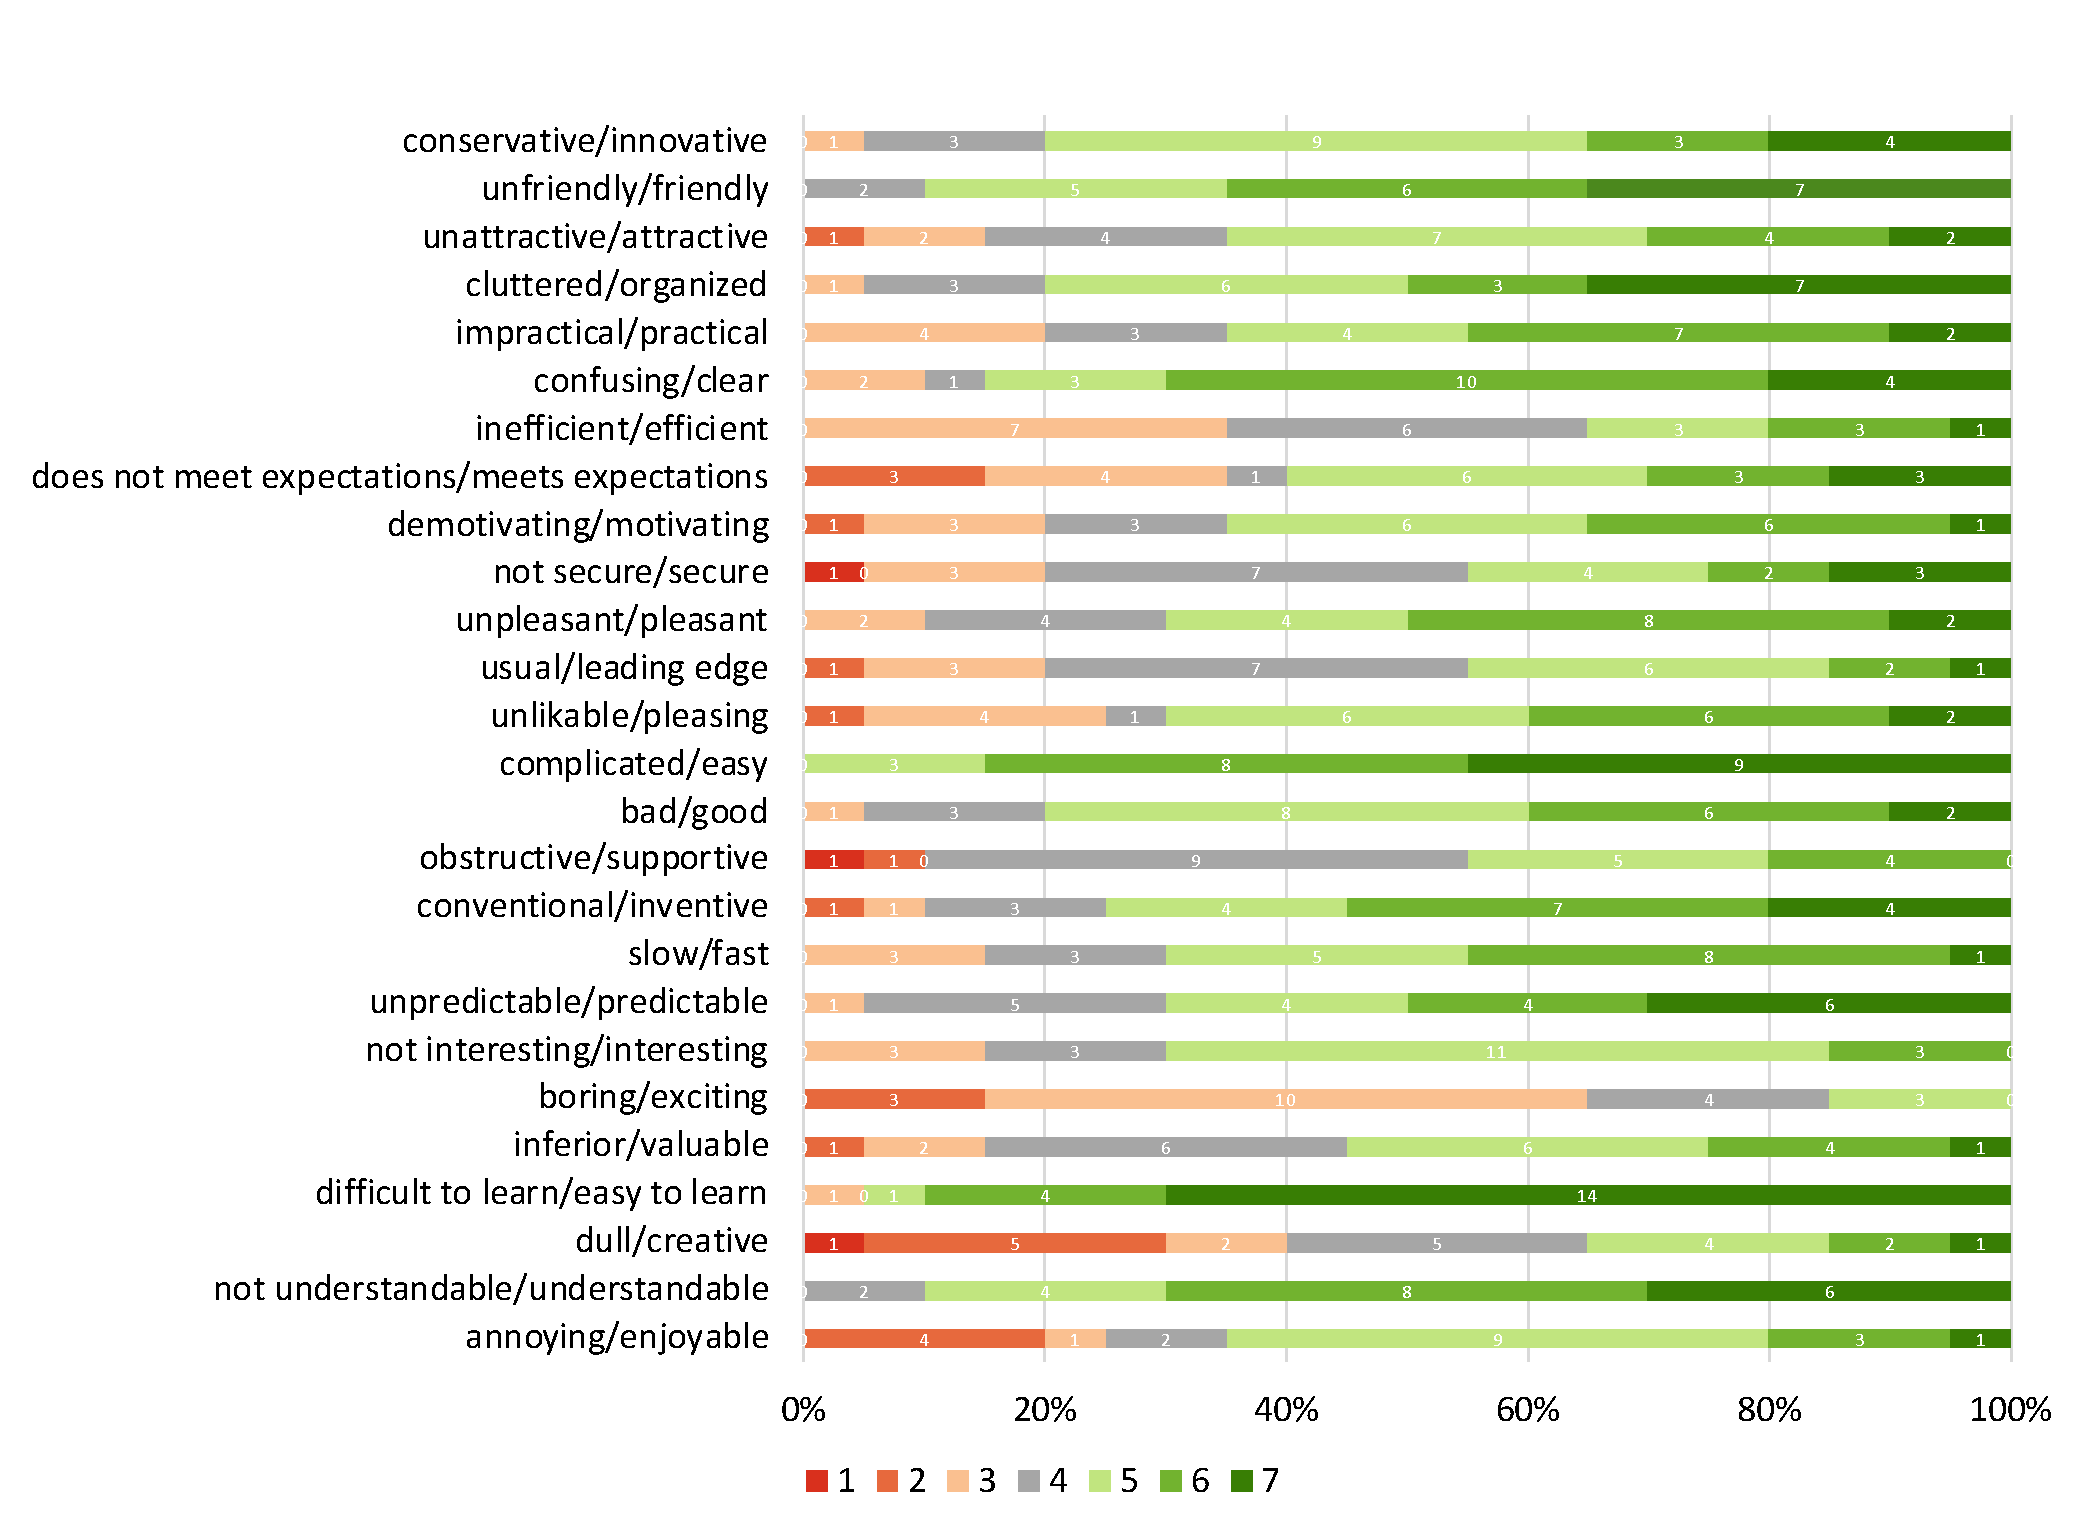
\includegraphics[clip, trim=0cm 0cm 0.25cm 0.25cm, width=\textwidth]{figures/ueq-distribution.pdf}
                \caption{Distribution of UEQ Answers per item (n=20). Labels 1 to 7 represent the spectrum of user's gradations between the opposite attributes of \acl{app} as such 1 denotes user's strong agreement with the negative attribute, 7 reflects positive impression and 4 indicates neutral sentiment. For example, users' response 1 to UEQ item `conservative/innovative' means their agreement that the system is conservative, 7 indicates that the system is innovative, and 4 represents users' neutral feedback. Annotations within the distribution represent the frequency of users' score.}
                \label{fig:ueq-distribution}
            \end{figure}
        
        Table \ref{tab:ueq_summary} shows the statistical summary of the participants' response to \ac{UEQ} scale.
        
        
                \begin{table}[t]
                \centering
                \caption{Statistical summary of the \ac{UEQ} scores. Confidence intervals (p=0.05) per scale.}
                \begin{tabular}{p{2cm} p{1cm} p{2cm} p{1cm} p{2cm} p{2cm} p{1.25cm}}
                    \toprule
                    \textbf{Scale}	& \textbf{Mean}	& \textbf{Std. Dev.}	& \textbf{N}	    & \textbf{Confidence}	& \multicolumn{2}{l}{\textbf{Confidence Interval}}\\
                    \midrule
                    Attractiveness	& 1.092	& 1.015	    & 20	& 0.445	        & 0.647	    & 1.537\\
                    Perspicuity	    & 2.088	& 0.749	    & 20	& 0.328	        & 1.759	    & 2.416\\
                    Efficiency	    & 0.975	& 0.773	    & 20	& 0.339	        & 0.636	    & 1.314\\
                    Dependability	& 0.738	& 0.837	    & 20	& 0.367	        & 0.371	    & 1.104\\
                    Stimulation	    & 0.375	& 0.817	    & 20	& 0.358	        & 0.017	    & 0.733\\
                    Novelty	        & 0.713	& 0.878	    & 20	& 0.385	        & 0.328	    & 1.097\\
                    \bottomrule
                \end{tabular}
                \label{tab:ueq_summary}
            \end{table}
        
        % \begin{figure}
        %     \centering
        %     \centering
        %     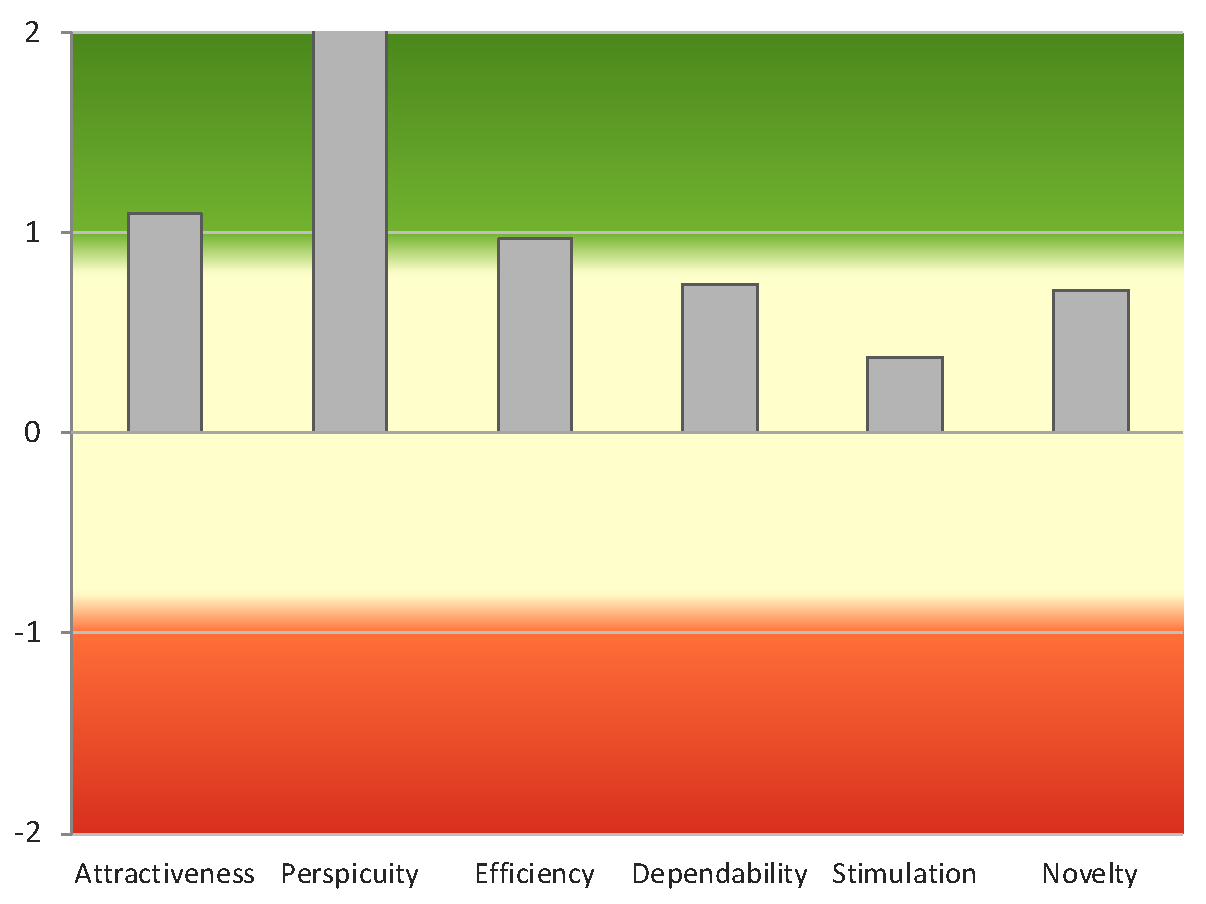
\includegraphics[width=0.75\textwidth]{figures/ueq-mean.pdf}
        %     \captionof{figure}{Participant's mean \ac{UEQ} scores aggregated into six dimensions attractiveness, perspicuity, efficiency, dependability, stimulation and novelty}
        %     \label{fig:ueq-mean}
        % \end{figure}
        
        Figure~\ref{fig:ueq-benchmark} illustrates the \ac{CA}'s \ac{UEQ} score compared to the benchmark data. The figure shows that the \ac{CA} is rated `excellent' for perspicuity which means that the rating is in the range of the 10\% of the best results in the benchmark data. Attractiveness, efficiency, and novelty were rated as `below average' which means 50\% of the results in the benchmark are better than the result for the evaluated system and 25\% of the results are worse. Finally, dependability and stimulation were rated as `bad' meaning that the the system is rated in range of the 25\% worst results in the benchmark data.
        \begin{figure}
            \centering
            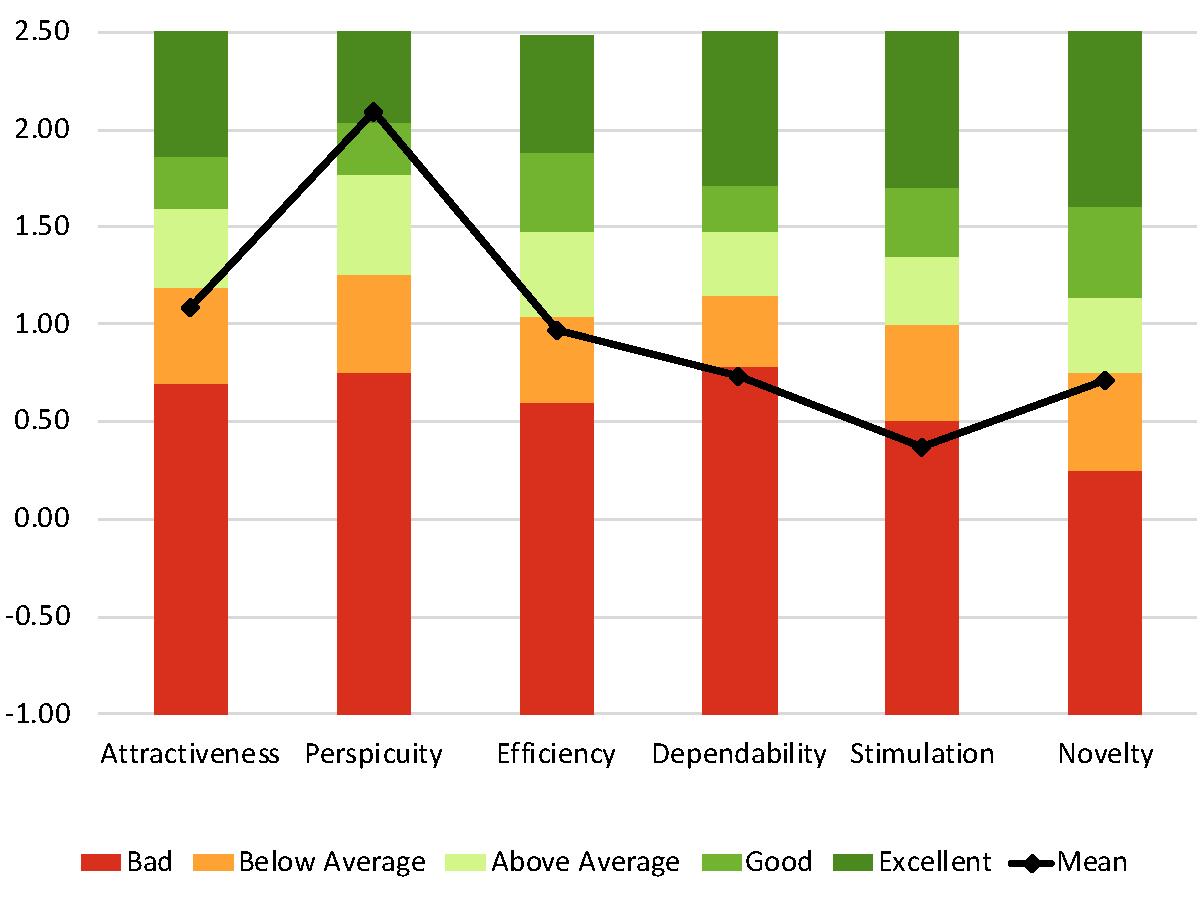
\includegraphics[width=0.7\textwidth]{figures/ueq-benchmark.pdf}
            \captionof{figure}{Comparison of the users scores for \acl{app} in each \ac{UEQ} dimension with the benchmark.
            }
            \label{fig:ueq-benchmark}
        \end{figure}
        
        
        The internal consistency of the \ac{UEQ} dimensions measured by Cronbach-Alpha in our evaluation resulted sufficient in terms of attractiveness ($\alpha = 0.89$), perspicuity ($\alpha = 0.76$) and stimulation ($\alpha = 0.73$). Whereas, the Cronbach-Alpha values for efficiency ($\alpha = 0.44$), dependability ($\alpha = 0.29$) and novelty ($\alpha = 0.57$) indicate poor internal consistency suggesting that the several participants might have interpreted the questions differently in the given context.
            
            
        
            
        

        

        






% \section{Research Methods}

% \subsection{Part One}

% Lorem ipsum dolor sit amet, consectetur adipiscing elit. Morbi
% malesuada, quam in pulvinar varius, metus nunc fermentum urna, id
% sollicitudin purus odio sit amet enim. Aliquam ullamcorper eu ipsum
% vel mollis. Curabitur quis dictum nisl. Phasellus vel semper risus, et
% lacinia dolor. Integer ultricies commodo sem nec semper.

% \subsection{Part Two}

% Etiam commodo feugiat nisl pulvinar pellentesque. Etiam auctor sodales
% ligula, non varius nibh pulvinar semper. Suspendisse nec lectus non
% ipsum convallis congue hendrerit vitae sapien. Donec at laoreet
% eros. Vivamus non purus placerat, scelerisque diam eu, cursus
% ante. Etiam aliquam tortor auctor efficitur mattis.

% \section{Online Resources}

% Nam id fermentum dui. Suspendisse sagittis tortor a nulla mollis, in
% pulvinar ex pretium. Sed interdum orci quis metus euismod, et sagittis
% enim maximus. Vestibulum gravida massa ut felis suscipit
% congue. Quisque mattis elit a risus ultrices commodo venenatis eget
% dui. Etiam sagittis eleifend elementum.

% Nam interdum magna at lectus dignissim, ac dignissim lorem
% rhoncus. Maecenas eu arcu ac neque placerat aliquam. Nunc pulvinar
% massa et mattis lacinia.
% \makeglossaries
\end{document}
\endinput
%%
